\documentclass[10pt,a4paper,twoside]{article}
\usepackage{pstricks}
\usepackage{fancybox}
\usepackage{amsfonts}
% \usepackage{minitoc}
% \setcounter{minitocdepth}{2}
\usepackage[bookmarks=true, 
            bookmarksnumbered=true, 
            bookmarksopen=false, 
            plainpages=false,
            pdfpagelabels,
            colorlinks, 
            linkcolor=blue]{hyperref}
\usepackage{ifthen}
\usepackage{graphicx}
\newtheorem{theorem}{Theorem}
\newtheorem{corollary}{Corollary}
\usepackage{listings}

%\newboolean{mtc}
%\setboolean{mtc}{true}

\pdfoutput=0
% \relax
% \pdfcompresslevel=0             %-- 0 = none, 9 = best
% \pdfinfo{                       %-- Info dictionary of PDF output  /Author (Alfredo Buttari)
%   /Title (Parallel Sparse BLAS V. 3.5.0)
%   /Subject (Parallel Sparse Basic Linear Algebra Subroutines)
%   /Keywords (Computer Science Linear Algebra Fluid Dynamics Parallel Linux MPI PSBLAS Iterative Solvers Preconditioners)
%   /Creator (pdfLaTeX)
%   /Producer ($Id: userguide.tex 1978 2007-10-19 14:51:12Z sfilippo $)
% }
% \pdfcatalog{          %-- Catalog dictionary of PDF output.
%   /URI (http://ce.uniroma2.it/psblas)
% } 

\newcounter{subroutine}[subsection]
\newcounter{example}[subroutine]
\makeatletter
\def\subroutine{\@ifstar{\@subroutine}{\clearpage\@subroutine}}%
\def\@subroutine#1#2{%
\stepcounter{subroutine}%
      \section*{\flushleft #1---#2 \endflushleft}%
      \addcontentsline{toc}{subsection}{#1}%
      \markright{#1}}%
\newcommand{\subsubroutine}[2]{%
\stepcounter{subroutine}%
      \subsection*{\flushleft #1---#2 \endflushleft}%
      \addcontentsline{toc}{subsubsection}{#1}%
      \markright{#1}}%
\newcommand{\subsubsubroutine}[2]{%
\stepcounter{subroutine}%
      \subsubsection*{\flushleft #1---#2 \endflushleft}%
      \addcontentsline{toc}{paragraph}{#1}%
      \markright{#1}}%
\newcommand{\examplename}{Example}
\newcommand{\syntaxname}{Syntax}
\def\syntax{\@ifstar{\@ssyntax}{\@syntax}}%
\def\@syntax{\nobreak\section*{\syntaxname}%
     \@ssyntax}%
\def\@ssyntax#1#2{%
  \nobreak
   \setbox\@tempboxa\hbox{#1\ {\em $($#2$)$}}%
   \ifdim \wd\@tempboxa >\hsize
        \setbox\@tempboxa\hbox{\em $($#2$)$}
	\ifdim\wd\@tempboxa >\hsize
          \flushright#1\ \em$($#2$)$\endflushright%
	\else
         \hbox to\hsize{#1\hfil}%
         \hbox to\hsize{\hfil\box\@tempboxa}%
        \fi
     \else
       \hbox to\hsize{\hfil\box\@tempboxa\hfil}%
   \fi\par\vskip\baselineskip}
\makeatother
\newcommand{\example}{\stepcounter{example}%
\section*{\examplename~\theexample}}

\newcommand{\precdata}{\hyperlink{precdata}{{\tt psb\_prec\_type}}}
\newcommand{\descdata}{\hyperlink{descdata}{{\tt psb\_desc\_type}}}
\newcommand{\spdata}{\hyperlink{spdata}{{\tt psb\_Tspmat\_type}}}
\newcommand{\vdata}{\hyperlink{vdata}{{\tt psb\_T\_vect\_type}}}
\newcommand{\spbasedata}{\hypertarget{spbasedata}{{\tt psb\_T\_base\_sparse\_mat}}}
\newcommand{\vbasedata}{\hypertarget{vbasedata}{{\tt psb\_T\_base\_vect\_type}}}

\begin{document}
\lstset{language=Fortran}

{\LARGE\bfseries PSBLAS\\[.8ex] User's and Reference
  Guide}\\[\baselineskip]
\emph{\large A reference guide for the Parallel Sparse BLAS library}\\[3ex]
{\bfseries Salvatore Filippone\\
   Alfredo Buttari } \\
%\\[10ex]
%\today
Software version: 3.5.0\\
%\today
Sep 1st, 2017
\cleardoublepage
\begingroup
  \renewcommand*{\thepage}{toc}
  \pagenumbering{roman}   % Roman numbering
  \setcounter{page}{1}    % Abstract start on page ii
  \tableofcontents
\endgroup  

\cleardoublepage

\pagenumbering{arabic}  % Arabic numbering
\setcounter{page}{1}    % Chapters start on page 1

\section{Introduction}\label{sec:intro}

The PSBLAS library, developed with the aim to facilitate the
parallelization of computationally intensive scientific applications,
is designed to address parallel implementation of iterative solvers
for sparse linear systems through the distributed memory paradigm.  It
includes routines for multiplying sparse matrices by dense matrices,
solving block diagonal systems with triangular diagonal entries,
preprocessing sparse matrices, and contains additional routines for
dense matrix operations.  The current implementation of PSBLAS
addresses a distributed memory execution model operating with message
passing. 

The PSBLAS library version 3 is  implemented in
 the Fortran~2003~\cite{metcalf} programming language, with reuse and/or
 adaptation of  existing Fortran~77 and Fortran~95 software, plus a
 handful of C  routines. 

The use of Fortran~2003 offers a number of advantages over Fortran~95,
mostly in the handling of requirements for evolution and adaptation of
the library to new computing architectures and integration of
new algorithms. 
For a detailed discussion of our design see~\cite{Sparse03}; other
works discussing advanced programming in Fortran~2003
include~\cite{DesPat:11,RouXiaXu:11}; sufficient support for
Fortran~2003 is now available from many compilers, including the GNU
Fortran compiler from the Free Software Foundation (as of version 4.6). 


Previous approaches have been based on mixing Fortran~95, with its
support for object-based design, with other languages; these have
been advocated by a number of authors, 
e.g.~\cite{machiels}.  Moreover, the Fortran~95 facilities for dynamic
memory management and interface overloading greatly enhance the
usability of the PSBLAS 
subroutines. In this way, the library can take care of runtime memory
requirements that are quite difficult or even impossible to predict at
implementation or compilation time.  

The presentation of the
PSBLAS library follows the general structure of the proposal for
serial Sparse BLAS~\cite{sblas97,sblas02}, which in its turn is based on the
proposal for BLAS on dense matrices~\cite{BLAS1,BLAS2,BLAS3}.

The applicability of sparse iterative solvers to many different areas
causes some terminology problems because the same concept may be
denoted through different names depending on the application area. The
PSBLAS features presented in this document will be discussed referring
to a   finite difference discretization of a Partial Differential
Equation (PDE). However, the scope of the library is wider than
that: for example, it can be applied to finite element discretizations
of PDEs, and even to different classes of problems such as nonlinear
optimization, for example in optimal control problems.

The design of a solver for sparse linear systems is driven by many
conflicting objectives, such as limiting occupation of storage
resources, exploiting regularities in the input data, exploiting
hardware characteristics of the parallel platform.  To achieve an
optimal communication to computation ratio on distributed memory
machines it is essential to keep the {\em data locality} as high as
possible; this can be done through an appropriate data allocation
strategy.  The choice of the preconditioner is another very important
factor that affects efficiency of the implemented application. Optimal
data distribution requirements for a given preconditioner may conflict
with distribution requirements of the rest of the solver. Finding the
optimal trade-off may be very difficult because it is application
dependent.  Possible solutions to these problems and other important
inputs to the development of the PSBLAS software package have come from
an established experience in applying the PSBLAS solvers to
computational fluid dynamics applications.

\section{General overview}
\label{sec:overview} 
The PSBLAS library is designed to handle the implementation of
iterative solvers for sparse linear systems on distributed memory
parallel computers.  The system coefficient matrix $A$ must be square;
it may be real or complex, nonsymmetric, and its sparsity pattern
needs not to be symmetric.  The serial computation parts are based on
the serial sparse BLAS, so that any extension made to the data
structures of the serial kernels is available to the parallel
version. The overall design and parallelization strategy have been
influenced by the structure of the ScaLAPACK parallel
library.  The layered structure of the PSBLAS library
is shown in figure~\ref{fig:psblas}; lower layers of the library
indicate an encapsulation relationship with upper layers. The ongoing
discussion focuses on the Fortran~2003 layer immediately below the
application layer.
The serial parts of the computation on each process are executed through
calls to the serial sparse BLAS subroutines. 
In a similar way, the inter-process message exchanges are encapsulated
in an applicaiton layer that has been strongly inspired by the  Basic
Linear Algebra Communication Subroutines (BLACS) library~\cite{BLACS}.  
Usually  there is no need to deal directly with MPI;  however, in some
cases, MPI routines are used directly to improve efficiency. For
further details on our communication layer see Sec.~\ref{sec:parenv}.
%% We assume that the user program has initialized a BLACS process grid
%% with one column and as many rows as there are processes; the PSBLAS
%% initialization routines will take the communication context for this
%% grid and store internally for further use. 

\begin{figure}[h] 
\begin{center}
\ifcase\pdfoutput
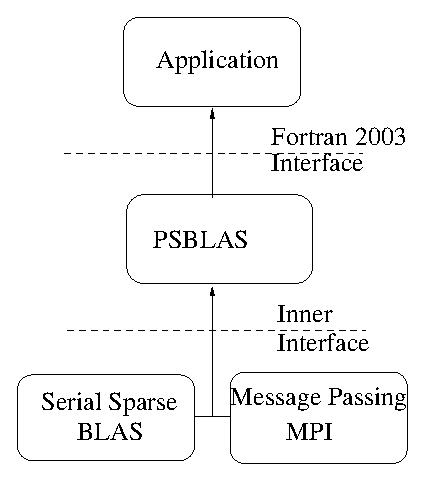
\includegraphics[scale=0.65]{figures/psblas.eps}
\or
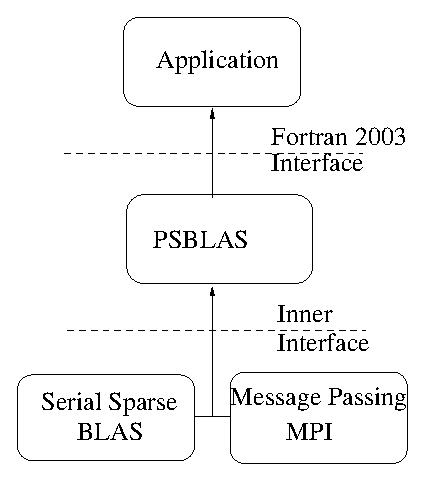
\includegraphics[scale=0.65]{figures/psblas}
\fi
\end{center}
\caption{PSBLAS library components hierarchy.\label{fig:psblas}}
\end{figure}


The type of linear system matrices that we address  typically arise in the
numerical solution of PDEs;  in such a context,
it is necessary to pay special attention to the
structure of the problem from which the application originates. 
The nonzero pattern of a matrix arising from the
discretization of a PDE is influenced by various factors, such as the
shape of the  domain, the discretization strategy, and
the equation/unknown ordering. The matrix itself can be interpreted as
the  adjacency matrix of the graph associated with the discretization
mesh. 

The distribution of the coefficient matrix for the linear system is
based on the ``owner computes'' rule: 
the variable associated to each mesh point is assigned to a process
that will  own the corresponding row in the coefficient matrix and
will  carry out all related computations. This allocation strategy 
is equivalent to a partition of the discretization mesh into {\em
sub-domains}. 
Our library  supports any distribution that keeps together 
the coefficients of each matrix row; there are no other constraints on
the variable assignment. 
This choice is consistent with simple  data distributions 
%commonly used in ScaLAPACK 
such as  \verb|CYCLIC(N)| and \verb|BLOCK|, 
as well as completely arbitrary assignments of
equation indices to processes. 
In particular it is consistent with the
usage of graph partitioning tools commonly available in the
literature, e.g. METIS~\cite{METIS}.
Dense vectors  conform  to sparse
matrices, that is, the entries of a vector follow the same distribution
of the matrix rows.  

We assume that the sparse matrix is built in parallel, where each
process generates its own portion. We never require that the entire
matrix be available on a single node. However, it is possible
to hold the entire matrix in one process and distribute it
explicitly\footnote{In our prototype implementation  we provide 
sample scatter/gather routines.}, even though  the resulting memory 
bottleneck would make this option unattractive in most  cases. 


\subsection{Basic Nomenclature}


Our computational model implies that the data allocation on the
parallel distributed memory machine is guided by the structure of the
physical model, and specifically by the discretization mesh of the
PDE. 

Each point of the discretization mesh will have (at least) one
associated equation/variable, and therefore one index. We say that
point  $i$ {\em depends\/} on point $j$ if the  equation for a
variable associated with $i$ contains a term in $j$,  or equivalently
if $a_{ij} \ne0$.  
After the partition of the discretization mesh into {\em sub-domains\/}
assigned to the parallel processes,
we classify the  points of a given sub-domain as following.
\begin{description}
\item[Internal.] An internal point of
 a given domain {\em depends} only on  points of the
same domain. 
If all points of a domain are assigned to one
process, then a computational step (e.g., a
matrix-vector product) of the 
equations associated with the internal points  requires no data
items from other domains and no communications.

\item[Boundary.] A point of
a given domain is a boundary point if it {\em depends} on  points
belonging to other domains.

\item[Halo.] A halo point for a given domain is a point belonging to
another domain such that there is a boundary point which {\em depends\/}
on it. Whenever performing a computational step, such as a
matrix-vector product, the values associated with halo points are
requested from other domains. A boundary point of a given 
domain is usually a halo point for some other domain\footnote{This is
  the normal situation when the pattern of the sparse matrix is
  symmetric, which is equivalent to say that the interaction between
  two variables is reciprocal. If the matrix pattern is non-symmetric
  we may have one-way interactions, and these could cause a situation
  in which a boundary point is not a halo point for its neighbour.}; therefore
the cardinality of the boundary points set denotes the amount of data
 sent to other domains. 
\item[Overlap.] An overlap point is a boundary point assigned to
multiple domains. Any operation that involves an overlap point
has to be replicated for each assignment. 
\end{description}
Overlap points do not usually exist in the basic data
distributions; however they are a feature of Domain Decomposition
Schwarz preconditioners which are the subject of related research
work~\cite{2007c,2007d}.

We denote the sets of  internal, boundary and halo points for a given
subdomain  by $\cal I$, $\cal B$ and $\cal H$.
Each subdomain is assigned to one process; each process usually
owns one subdomain, although the user may choose to assign more than
one subdomain to a process.  If each process $i$ owns one
subdomain, the number of rows in the local sparse matrix is
$|{\cal I}_i| + |{\cal B}_i|$, and the number of local columns
(i.e. those for which there exists at least one non-zero entry in the
local rows)  is $|{\cal I}_i| + |{\cal B}_i| +|{\cal H}_i|$.

\begin{figure}[h] 
\begin{center}
\ifcase\pdfoutput
%\rotatebox{-90}{
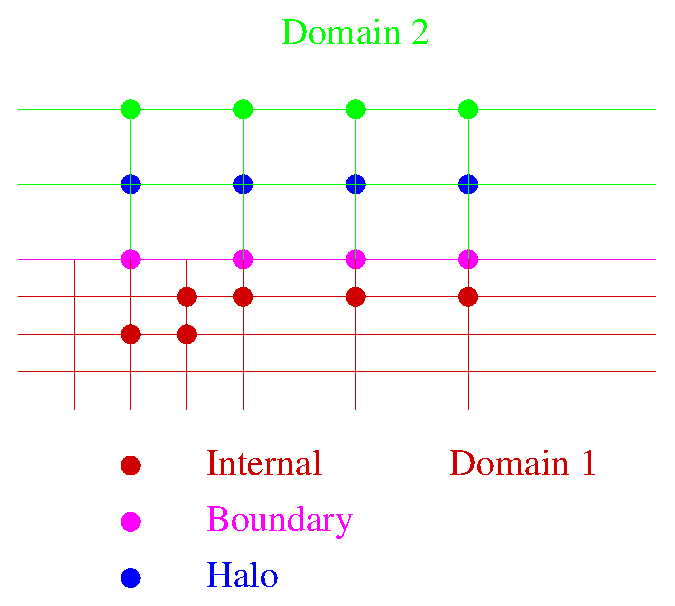
\includegraphics[scale=0.65]{figures/points.eps}%}
\or
\rotatebox{-90}{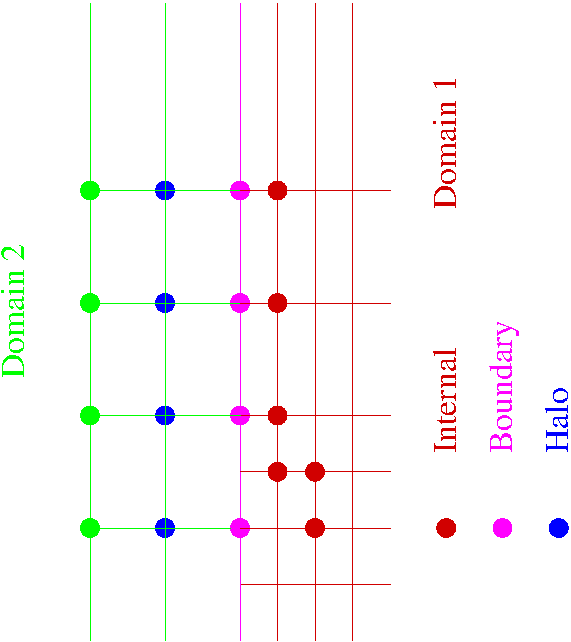
\includegraphics[scale=0.65]{figures/points}}
\fi
\end{center}
\caption{Point classfication.\label{fig:points}}
\end{figure}

This classification of mesh points guides the naming scheme that we
adopted in the library internals and in the data structures. We
explicitly note that ``Halo'' points are also often called ``ghost''
points in the literature. 



\subsection{Library contents}

The PSBLAS library consists of various classes of subroutines:
\begin{description}
\item[Computational routines] comprising:
\begin{itemize}
\item Sparse matrix by dense matrix product; 
\item Sparse triangular
systems solution for block diagonal matrices;
\item Vector and matrix norms;
\item Dense matrix sums;
\item Dot products.
\end{itemize} 
\item[Communication routines] handling halo and overlap
  communications;
\item[Data management and auxiliary routines] including:
\begin{itemize}
\item Parallel environment management
\item Communication descriptors allocation;
\item Dense and sparse matrix allocation;
\item Dense and sparse matrix build and update;
\item Sparse matrix and data distribution preprocessing.
\end{itemize} 
\item[Preconditioner routines]
\item[Iterative methods] a subset of Krylov subspace iterative
  methods
\end{description}
The following naming scheme has been adopted for all the symbols
internally defined in the PSBLAS software package:
\begin{itemize}
\item all symbols (i.e. subroutine names, data types...) are
  prefixed by \verb|psb_| 
\item all data type names are suffixed by \verb|_type|
\item all constants are suffixed by \verb|_|
\item all top-level subroutine names follow the rule \verb|psb_xxname| where
  \verb|xx| can be either:
  \begin{itemize}
  \item \verb|ge|: the routine is related to dense data, 
  \item \verb|sp|: the routine is related to sparse data, 
  \item \verb|cd|: the routine is related to communication descriptor
        (see~\ref{sec:datastruct}).
  \end{itemize}
  For example the \verb|psb_geins|, \verb|psb_spins| and
  \verb|psb_cdins| perform the same action (see~\ref{sec:toolsrout}) on
  dense matrices, sparse matrices and communication descriptors
  respectively.
  Interface overloading allows the usage of the same subroutine
  names  for both real and complex data.
\end{itemize}
In the description of the subroutines, arguments or argument entries
are classified as:
\begin{description}
\item[global] For input arguments, the value must be the same on all processes
  participating in the subroutine call; for output arguments the value
  is guaranteed to be the same.
\item[local] Each process has its own value(s) independently.
\end{description}
To finish our general description, we define a version string with the
constant 
\[ \verb|psb_version_string_|\]
whose current value is \verb|3.0.0|

\subsection{Application structure}
\label{sec:appstruct}

The main underlying principle of the PSBLAS library is that the
library objects are created and exist with reference to a discretized
space to which there corresponds an index space and a matrix sparsity
pattern. As an example, consider a cell-centered finite-volume
discretization of  the Navier-Stokes equations on a simulation domain;
the index space $1\dots n$ is isomorphic to the set of cell centers,
whereas the pattern of the associated linear system matrix is
isomorphic to the adjacency graph imposed on the discretization mesh
by the discretization stencil. 

Thus the first order of business is to establish an index space, and
this is done with a call to  \verb|psb_cdall| in which we specify the
size of the index space $n$ and the allocation of the elements of the
index space to the various processes making up the MPI (virtual)
parallel machine. 

The index space is partitioned among processes, and this creates a
mapping from the ``global'' numbering $1\dots n$ to a numbering
``local'' to each process; each process $i$ will own a certain subset
$1\dots n_{\hbox{row}_i}$, each element of which corresponds to a certain
element of $1\dots n$. The user does not set explicitly this mapping;
when the application needs to indicate to which element of the index
space a certain item is related, such as the row and column index of a
matrix coefficient, it does so in the ``global'' numbering, and the
library will translate into the appropriate ``local'' numbering. 

For  a given index space $1\dots n$ there are many possible associated
topologies, i.e. many different discretization stencils; thus the
description of the index space is not completed until the user has
defined a sparsity pattern, either explicitly through \verb|psb_cdins|
or implicitly through \verb|psb_spins|. The descriptor is finalized
with a call to \verb|psb_cdasb| and a sparse matrix with a call to
\verb|psb_spasb|. After \verb|psb_cdasb| each process $i$ will have
defined a set of ``halo'' (or ``ghost'') indices
$n_{\hbox{row}_i}+1\dots n_{\hbox{col}_i}$, denoting elements of the index
space that are \emph{not} assigned to process $i$; however the
variables associated with them are needed to complete computations
associated with the sparse matrix $A$, and thus they have to be
fetched from (neighbouring) processes. The descriptor of the index
space is built exactly for the purpose of properly sequencing the
communication steps required to achieve this objective. 

A simple application structure will walk through the index space
allocation, matrix/vector creation and linear system solution as
follows:
\begin{enumerate}
\item Initialize parallel environment with \verb|psb_init|
\item Initialize index space with \verb|psb_cdall|
\item Allocate sparse matrix and dense vectors with \verb|psb_spall|
  and \verb|psb_geall|
\item Loop over all local rows, generate matrix and vector entries,
  and insert them with \verb|psb_spins| and \verb|psb_geins|
\item Assemble the various entities: 
\begin{enumerate}
\item \verb|psb_cdasb|
\item \verb|psb_spasb|
\item \verb|psb_geasb|
\end{enumerate}
\item Choose the preconditioner to be used with \verb|psb_precset| and
  build it with \verb|psb_precbld|
\item Call the iterative method of choice, e.g. \verb|psb_bicgstab|
\end{enumerate}
This is the structure of the sample program
\verb|test/pargen/ppde.f90|. 

For a simulation in which the same discretization mesh is used over
multiple time steps, the following structure may be more appropriate:
\begin{enumerate}
\item Initialize parallel environment with \verb|psb_init|
\item Initialize index space with \verb|psb_cdall|
\item Loop over the topology of the discretization mesh and build the
  descriptor with \verb|psb_cdins|
\item Assemble the descriptor with \verb|psb_cdasb|
\item Allocate the sparse matrices and dense vectors with
  \verb|psb_spall| and \verb|psb_geall|
\item Loop over the time steps: 
\begin{enumerate}
\item If after first time step, 
  reinitialize the sparse matrix with \verb|psb_sprn|; also zero out
  the dense vectors;
\item Loop over the mesh, generate the coefficients and insert/update
  them with \verb|psb_spins| and \verb|psb_geins|
\item Assemble with \verb|psb_spasb| and \verb|psb_geasb|
\item Choose and build preconditioner with \verb|psb_precset| and
  \verb|psb_precbld|
\item Call the iterative method of choice, e.g. \verb|psb_bicgstab|
 \end{enumerate}
\end{enumerate}
The insertion routines will be called as many times as needed; 
they only need to  be called on the data that is actually
allocated to the current process, i.e. each process generates its own
data. 

In principle there is no specific order in the calls to
\verb|psb_spins|, nor is there a requirement to build a matrix row in
its entirety before calling the routine; this allows the application
programmer to walk through the discretization mesh element by element,
generating the main part of a given matrix row but also contributions
to the rows corresponding to neighbouring elements. 

From a functional point of view it is even possible to execute one
call for each nonzero coefficient; however this would have a
substantial computational overhead. It is therefore advisable to pack
a certain amount of data into each call to the insertion routine, say
touching on a few tens of rows; the best performng value would depend
on both the architecture of the computer being used and on the problem
structure. 
At the opposite extreme, it would be possible to generate the entire
part of a coefficient matrix residing on a process and pass it in a
single call to \verb|psb_spins|; this, however, would entail a
doubling of memory occupation, and thus would be almost always far
from optimal. 

\subsubsection{User-defined index mappings}
\label{sec:usermaps}
PSBLAS supports user-defined global to local index mappings, subject
to the constraints outlined in sec.~\ref{sec:appstruct}: 
\begin{enumerate}
\item The set of indices owned locally must be mapped to the set
  $1\dots n_{\hbox{row}_i}$;
\item The set of halo points must be mapped to the set
  $n_{\hbox{row}_i}+1\dots n_{\hbox{col}_i}$;
\end{enumerate}
but otherwise the mapping is arbitrary. The user application is
responsible to ensure consistency of this mapping; some errors may be
caught by the library, but this is not guaranteed. 
The application structure to
support this usage is as follows:
\begin{enumerate}
\item Initialize index space with
  \verb|psb_cdall(ictx,desc,info,vl=vl,lidx=lidx)| passing the vectors 
  \verb|vl(:)| containing the set of global indices owned by the
  current process and   \verb|lidx(:)| containing the corresponding
  local indices;
\item Add the halo points \verb|ja(:)| and their associated local
  indices \verb|lidx(:)|  with a(some) call(s) to
  \verb|psb_cdins(nz,ja,desc,info,lidx=lidx)|; 
\item Assemble the descriptor with \verb|psb_cdasb|;
\item Build the sparse matrices and vectors, optionally making use in
  \verb|psb_spins| and \verb|psb_geins| of the \verb|local| argument
  specifying that the indices in \verb|ia|, \verb|ja| and \verb|irw|,
  respectively, are already local indices. 
\end{enumerate}


\subsection{Programming model}

The PSBLAS librarary is based on the Single Program Multiple Data
(SPMD) programming model: each process participating in the
computation performs the same actions on a chunk of data. Parallelism
is thus data-driven. 

Because of this structure, many subroutines coordinate their action
across the various processes, thus providing an implicit
synchronization point, and therefore \emph{must} be
called simultaneously by all processes participating in the
computation. This is certainly true for the data allocation and
assembly routines, for  all the computational routines and for some of
the tools routines.

However there are many cases where no synchronization, and indeed no
communication among processes, is implied; for instance, all the routines in
sec.~\ref{sec:dataquery} are only acting on the local data structures,
and thus may be called independently. The most important case is that
of the coefficient insertion routines: since the number of
coefficients in the sparse and dense matrices varies among the
processors, and since the user is free to choose an arbitrary order in
builiding the matrix entries, these routines cannot imply a
synchronization. 

Throughout this user's guide each subroutine will be clearly indicated
as:
\begin{description}
\item[Synchronous:] must be called simultaneously by all the
  processes in the relevant communication context;
\item[Asynchronous:] may be called in a totally independent manner.
\end{description}

%%% Local Variables: 
%%% mode: latex
%%% TeX-master: "userguide"
%%% End: 

\section{Data Structures and Classes}
\label{sec:datastruct}
%\ifthenelse{\boolean{mtc}}{\minitoc}{}

In this chapter we  illustrate the  data structures used for definition of
routines interfaces. They  include data structures for sparse matrices,
communication descriptors and preconditioners.%%  These data structures
%% are used for calling PSBLAS routines in Fortran~90 language and will
%% be used to next chapters containing these callings.  

All the data types and the basic subroutine interfaces related to
descriptors and sparse matrices are defined in
the module \verb|psb_base_mod|; this will have to be included by every
user subroutine that makes use of the library. The preconditioners are
defined in the module \verb|psb_prec_mod|

Integer, real and complex data types are parametrized with a kind type
defined in the library as follows: 
\begin{description}
\item[psb\_spk\_] Kind parameter for short precision real and complex
  data; corresponds to a \verb|REAL| declaration and is
  normally 4 bytes; 
\item[psb\_dpk\_] Kind parameter for long precision real and complex
  data; corresponds to a \verb|DOUBLE PRECISION| declaration and is
  normally 8 bytes;
\item[psb\_ipk\_] Kind parameter for integer data;
  with default build options this is a 4 bytes integer, but there is
  (highly) experimental support for 8-bytes integers;  
\item[psb\_mpik\_] Kind parameter for 4-bytes integer data, as is
  always used by MPI; 
\item[psb\_long\_int\_k\_] Kind parameter for long (8 bytes) integers, 
  which are always used by the \verb|sizeof| methods.
\end{description}
Together with the classes attributes we also discuss their
methods.  Most methods detailed here only act on the local variable,
i.e. their action is purely local and asynchronous unless otherwise
stated. 
The list of methods here is not completely exhaustive; many methods,
especially those that alter the contents of the various objects, are
usually not needed by the end-user, and therefore are described in the
developer's documentation. 


\subsection{Descriptor data structure}
\label{sec:desc}
All the general matrix informations and elements to be
exchanged among processes are stored within a data structure of the
type \hypertarget{descdata}{{\tt psb\_desc\_type}}. 
Every structure of this type is associated with a discretization
pattern and enables data communications and other operations that are
necessary for implementing the various algorithms of interest to us. 

The data structure itself \verb|psb_desc_type| can be treated as an
opaque object handled via the   tools routines of
Sec.~\ref{sec:toolsrout} or the query routines detailed below;
nevertheless we include here a  description for the curious 
reader. 

First we describe the \verb|psb_indx_map| type. This is a data
structure that keeps track of a certain number of basic issues such
as:
\begin{itemize}
\item The value of the communication/MPI context;
\item The number of indices in the index space, i.e. global number of
  rows and columns of a sparse matrix;
\item The local set of indices, including:
\begin{itemize}
\item The number of local indices (and local rows);
\item The number of halo indices (and therefore local columns); 
\item The global indices corresponding to the local ones. 
\end{itemize}
\end{itemize}
There are many different schemes for storing these data; therefore
there are a number of types extending the base one, and the descriptor
structure holds a polymorphic object whose dynamic type can be any of
the extended  types. 
The methods associated with this data type answer the following
queries:
\begin{itemize}
\item For a given set of local indices, find the corresponding indices
  in the global numbering;
\item For a given set of global indices, find the corresponding
  indices in the local numbering, if any, or return an invalid 
\item Add a global index to the set of halo indices;
\item Find the process  owner of each member of a set of global
  indices.
\end{itemize}
All methods but the last are purely local; the last method potentially
requires communication among processes, and thus is a synchronous
method. The choice of a specific dynamic type for the index map is
made at the time the descriptor is initially allocated, according to
the mode of initialization (see also~\ref{sec:toolsrout}).

The descriptor contents are as follows:
\begin{description}
\item[{\bf indxmap}] A polymorphic variable of a type that is any
  extension of the indx\_map type described above. \\
\item[{\bf halo\_index}] A list of the halo and boundary elements for
the current process to be exchanged with other processes; for each
processes with which it is necessary to communicate:
\begin{enumerate}
\item Process identifier;
\item Number of points to be received;
\item Indices of points to be received;
\item Number of points to be sent;
\item Indices of points to be sent;
\end{enumerate}
The list may contain an arbitrary number of groups; its end is marked
by a -1.\\
Specified as: an allocatable integer array of rank one.
\item[{\bf ext\_index}] A list of element indices to be exchanged to
  implement the mapping between a base descriptor and a descriptor
  with overlap. 
\item [{\bf ovrlap\_index}] A list of the overlap elements for the
current process, organized in groups like the previous vector:
\begin{enumerate}
\item Process identifier;
\item Number of points to be received;
\item Indices of points to be received;
\item Number of points to be sent;
\item Indices of points to be sent;
\end{enumerate}
The list may contain an arbitrary number of groups; its end is marked
by a -1.\\
Specified as: an allocatable integer array  of rank one.
\item [{\bf ovr\_mst\_idx}] A list to retrieve the value of each
  overlap element from the respective master process.\\
Specified as: an allocatable integer array of rank one.
\item [{\bf ovrlap\_elem}] For all overlap points belonging to th
ecurrent process:
\begin{enumerate}
\item Overlap point index;
\item Number of processes sharing that overlap points;
\item Index of a ``master'' process: 
\end{enumerate}
Specified as: an allocatable integer array of rank two.
\item [{\bf bnd\_elem}] A list of all boundary points, i.e. points
  that have a connection with other processes.
\end{description}
The Fortran~2003 declaration  for \verb|psb_desc_type| structures is 
as follows:
\begin{figure}[h!]
  % \begin{Sbox}
\begin{center}
    \begin{minipage}[tl]{0.9\textwidth}
\begin{verbatim} 
type psb_desc_type 
    class(psb_indx_map), allocatable :: indxmap
    integer, allocatable  :: halo_index(:)
    integer, allocatable  :: ext_index(:)
    integer, allocatable  :: ovrlap_index(:)
    integer, allocatable  :: ovrlap_elem(:,:)
    integer, allocatable  :: ovr_mst_idx(:)
    integer, allocatable  :: bnd_elem(:)
end type psb_desc_type 
\end{verbatim}
    \end{minipage}
  \end{center}
% \end{Sbox}
%   \setlength{\fboxsep}{8pt}
%   \begin{center}
%     \fbox{\TheSbox}
%   \end{center}
  \caption{\label{fig:desctype}The PSBLAS defined data type that
    contains the communication descriptor.}
\end{figure}

A communication descriptor associated with a sparse  matrix has a
state, which can take the following values:
\begin{description}
\item[Build:] State entered after the first allocation, and before the
  first assembly; in this state it is possible to add communication
  requirements among different processes. 
\item[Assembled:] State entered after the assembly; computations using
  the associated sparse matrix, such as matrix-vector products, are
  only possible   in this state.
\end{description}

\subsubsection{Descriptor Methods} 

\subsubsection*{get\_local\_rows --- Get number of local rows}
\addcontentsline{toc}{paragraph}{get\_local\_rows}

\begin{verbatim}
nr = desc%get_local_rows()
\end{verbatim}

\begin{description}
\item[Type:] Asynchronous.
\item[\bf On Entry]
\item[desc] the communication descriptor.\\
Scope: {\bf local}.\\
% Type: {\bf required}.\\
% Intent: {\bf in}.\\
% Specified as: a object of type \descdata.
\end{description}

\begin{description}
\item[\bf On Return]
\item[Function value] The number of local rows, i.e. the number of
  rows owned by the current process; as explained in~\ref{sec:intro},
  it is equal to $|{\cal I}_i| + |{\cal B}_i|$. The returned value is
  specific to the calling process. 
\end{description}


\subsubsection*{get\_local\_cols --- Get number of local cols}
\addcontentsline{toc}{paragraph}{get\_local\_cols}

\begin{verbatim}
nc = desc%get_local_cols()
\end{verbatim}

\begin{description}
\item[Type:] Asynchronous.
\item[\bf On Entry]
\item[desc] the communication descriptor.\\
Scope: {\bf local}.\\
% Type: {\bf required}.\\
% Intent: {\bf in}.\\
% Specified as: a object of type \descdata.
\end{description}

\begin{description}
\item[\bf On Return]
\item[Function value] The number of local cols, i.e. the number of
  indices used by the current process, including both local and halo
  indices; as explained in~\ref{sec:intro}, 
  it is equal to  $|{\cal I}_i| + |{\cal B}_i| +|{\cal H}_i|$. The
  returned value is specific to the calling process. 
\end{description}


\subsubsection*{get\_global\_rows --- Get number of global rows}
\addcontentsline{toc}{paragraph}{get\_global\_rows}

\begin{verbatim}
nr = desc%get_global_rows()
\end{verbatim}

\begin{description}
\item[Type:] Asynchronous.
\item[\bf On Entry]
\item[desc] the communication descriptor.\\
Scope: {\bf local}.\\
% Type: {\bf required}.\\
% Intent: {\bf in}.\\
% Specified as: a object of type \descdata.
\end{description}

\begin{description}
\item[\bf On Return]
\item[Function value] The number of global rows, i.e. the size of the
  global index space. 
\end{description}

\subsubsection*{get\_global\_cols --- Get number of global cols}
\addcontentsline{toc}{paragraph}{get\_global\_cols}

\begin{verbatim}
nr = desc%get_global_cols()
\end{verbatim}

\begin{description}
\item[Type:] Asynchronous.
\item[\bf On Entry]
\item[desc] the communication descriptor.\\
Scope: {\bf local}.\\
% Type: {\bf required}.\\
% Intent: {\bf in}.\\
% Specified as: a object of type \descdata.
\end{description}

\begin{description}
\item[\bf On Return]
\item[Function value] The number of global cols; usually this is equal
  to the number of global rows. 
\end{description}


\subsubsection*{get\_global\_indices --- Get vector of global indices}
\addcontentsline{toc}{paragraph}{get\_global\_rows}

\begin{verbatim}
myidx = desc%get_global_indices([owned])
\end{verbatim}

\begin{description}
\item[Type:] Asynchronous.
\item[\bf On Entry]
\item[desc] the communication descriptor.\\
Scope: {\bf local}.\\
Type: {\bf required}.\\
\item[owned] Choose if you only want owned indices
  (\verb|owned=.true.|) or also halo indices (\verb|owned=.false.|). 
Scope: {\bf local}.\\
Type: {\bf optional}; default: \verb|.true.|.\\
% Intent: {\bf in}.\\
% Specified as: a object of type \descdata.
\end{description}

\begin{description}
\item[\bf On Return]
\item[Function value] The global indices, returned as an allocatable
  integer array of rank 1. 
\end{description}



\subsubsection*{get\_context --- Get communication context}
\addcontentsline{toc}{paragraph}{get\_context}

\begin{verbatim}
ictxt = desc%get_context()
\end{verbatim}

\begin{description}
\item[Type:] Asynchronous.
\item[\bf On Entry]
\item[desc] the communication descriptor.\\
Scope: {\bf local}.\\
% Type: {\bf required}.\\
% Intent: {\bf in}.\\
% Specified as: a object of type \descdata.
\end{description}

\begin{description}
\item[\bf On Return]
\item[Function value] The communication context.
\end{description}

\subsubsection*{Clone --- clone current object}
\addcontentsline{toc}{paragraph}{Clone}

\begin{verbatim}
call  desc%clone(descout,info)
\end{verbatim}

\begin{description}
\item[Type:] Asynchronous.
\item[\bf On Entry]
\item[desc] the communication descriptor.\\
Scope: {\bf local}.\\
% Type: {\bf required}.\\
% Intent: {\bf in}.\\
% Specified as: a object of type \descdata.
\end{description}

\begin{description}
\item[\bf On Return]
\item[descout] A copy of the input object.
\item[info] Return code. 
\end{description}


\subsubsection*{psb\_cd\_get\_large\_threshold --- Get threshold for
  index mapping switch}
\addcontentsline{toc}{paragraph}{psb\_cd\_get\_large\_threshold}

\begin{verbatim}
ith = psb_cd_get_large_threshold()
\end{verbatim}

\begin{description}
\item[Type:] Asynchronous.
\item[\bf On Return]
\item[Function value] The current value for the size threshold. 

\end{description}



\subsubsection*{psb\_cd\_set\_large\_threshold --- Set threshold for
  index mapping switch}
\addcontentsline{toc}{paragraph}{psb\_cd\_set\_large\_threshold}

\begin{verbatim}
call psb_cd_set_large_threshold(ith)
\end{verbatim}

\begin{description}
\item[Type:] Synchronous.
\item[\bf On Entry]
\item[ith] the new threshold for communication descriptors.\\
Scope: {\bf global}.\\
Type: {\bf required}.\\
Intent: {\bf in}.\\
Specified as: an integer value greater than zero.
\end{description}
Note: the threshold value is only queried by the library at the time a
call to \verb|psb_cdall| is executed, therefore changing the threshold
has no effect on communication descriptors that have already been
initialized. Moreover the threshold must have the same value on all
processes. 

\subsubsection{Named Constants}
\label{sec:cd_constants}
\begin{description}
\item[psb\_none\_] Generic no-op;
\item[psb\_root\_] Default root process for broadcast and scatter operations;
\item[psb\_nohalo\_]  Do not fetch halo elements;
\item[psb\_halo\_]  Fetch halo elements from neighbouring processes;
\item[psb\_sum\_] Sum overlapped elements
\item[psb\_avg\_] Average overlapped elements
\item[psb\_comm\_halo\_] Exchange data based on the \verb|halo_index|
  list;
\item[psb\_comm\_ext\_] Exchange data based on the \verb|ext_index|
  list;
\item[psb\_comm\_ovr\_] Exchange data based on the \verb|ovrlap_index|
  list;
\item[psb\_comm\_mov\_] Exchange data based on the \verb|ovr_mst_idx|
  list;

%% \item[psb\_square\_root\_] Update with the square root of the average
%%   of overlapped elements;
%% \item[psb\_dec\_type\_] Entry holding decomposition type (in \verb|desc_a%matrix_data|)
%% \item[psb\_m\_] Entry holding total number of rows
%% \item[psb\_n\_] Entry holding total number of columns
%% \item[ psb\_n\_row\_] Entry holding the number of rows stored in the
%%   current process
%% \item[psb\_n\_col\_] Entry holding the number of columns stored in the
%%   current process
%% \item[psb\_ctxt\_] Entry holding a copy of the BLACS communication context
%% \item[psb\_desc\_asb\_] State of the descriptor: assembled,
%%       i.e. suitable for computational tasks. 
%% \item[psb\_desc\_bld\_] State of the descriptor: build, must be
%%   assembled before computational use.
\end{description}


\subsection{Sparse Matrix class}
\label{sec:spmat}
The \hypertarget{spdata}{{\tt psb\_Tspmat\_type}} class
contains all information about the local portion of the sparse matrix and   
its storage mode. Its design is 
based on the STATE design pattern~\cite{DesignPatterns} as detailed
in~\cite{Sparse03}; the type declaration is shown in
figure~\ref{fig:spmattype} where \verb|T| is a placeholder for the
data type and precision variants 
\begin{description}
\item[S] Single precision real;
\item[D] Double precision real;
\item[C] Single precision complex;
\item[Z] Double precision complex.
\end{description}
The actual data is contained in the polymorphic component \verb|a%a|
of type  \hypertarget{spbasedata}{{\tt psb\_T\_base\_sparse\_mat}}; its
specific layout can be chosen dynamically among the predefined types,
or an entirely new storage layout can be implemented and passed to the
library at runtime via the \verb|psb_spasb| routine. 
\begin{figure}[h!]
  % \begin{Sbox}
\begin{center}
    \begin{minipage}[tl]{0.85\textwidth}
\begin{verbatim}
  type :: psb_Tspmat_type
    class(psb_T_base_sparse_mat), allocatable  :: a 
  end type  psb_Tspmat_type
\end{verbatim}
    \end{minipage}
  \end{center}
% \end{Sbox}
%   \setlength{\fboxsep}{8pt}
%   \begin{center}
%     \fbox{\TheSbox}
%   \end{center}
  \caption{\label{fig:spmattype} 
    The PSBLAS defined data type that
    contains a sparse matrix.} 
\end{figure}
The following very common formats are precompiled in  PSBLAS and thus
are always available: 
\begin{description}
\item[psb\_T\_coo\_sparse\_mat] Coordinate storage; 
\item[psb\_T\_csr\_sparse\_mat] Compressed storage by rows; 
\item[psb\_T\_csc\_sparse\_mat] Compressed storage by columns; 
\end{description}
The inner sparse matrix has an associated state, which can take the
following values:
\begin{description}
\item[Build:] State entered after the first allocation, and before the
  first assembly; in this state it is possible to add nonzero entries.
\item[Assembled:] State entered after the assembly; computations using
  the sparse matrix, such as matrix-vector products, are only possible
  in this state;
\item[Update:] State entered after a reinitalization; this is used to
  handle applications in which the same sparsity pattern is used
  multiple times with different coefficients. In this state it is only
  possible to enter coefficients for already existing nonzero entries.
\end{description}
The only storage variant supporting the build state is COO; all other
variants are obtained by conversion to/from it. 

\subsubsection{Sparse Matrix Methods}

\subsubsection*{get\_nrows --- Get number of  rows in a sparse  matrix}
\addcontentsline{toc}{paragraph}{get\_nrows}

\begin{verbatim}
nr = a%get_nrows()
\end{verbatim}

\begin{description}
\item[Type:] Asynchronous.
\item[\bf On Entry]
\item[a] the sparse matrix\\
Scope: {\bf local}\\
% Type: {\bf required}\\
% Intent: {\bf in}.\\
% Specified as: a object of type \spdata.
\end{description}

\begin{description}
\item[\bf On Return]
\item[Function value] The number of  rows  of sparse matrix \verb|a|.
\end{description}


\subsubsection*{get\_ncols --- Get number of  columns in a  sparse
  matrix}
\addcontentsline{toc}{paragraph}{get\_ncols}

\begin{verbatim}
nc = a%get_ncols()
\end{verbatim}

\begin{description}
\item[Type:] Asynchronous.
\item[\bf On Entry]
\item[a] the sparse matrix\\
Scope: {\bf local}\\
% Type: {\bf required}\\
% Intent: {\bf in}.\\
% Specified as: a object of type \spdata.
\end{description}

\begin{description}
\item[\bf On Return]
\item[Function value] The number of  columns  of sparse matrix \verb|a|.
\end{description}


\subsubsection*{get\_nnzeros --- Get number of nonzero elements
  in a sparse matrix}
\addcontentsline{toc}{paragraph}{get\_nnzeros}

\begin{verbatim}
nz = a%get_nnzeros()
\end{verbatim}

\begin{description}
\item[Type:] Asynchronous.
\item[\bf On Entry]
\item[a] the sparse matrix\\
Scope: {\bf local}\\
% Type: {\bf required}\\
% Intent: {\bf in}.\\
% Specified as: a object of type \spdata.
\end{description}

\begin{description}
\item[\bf On Return]
\item[Function value] The number of nonzero elements stored in sparse matrix \verb|a|.
\end{description}

{\par\noindent\bfseries Notes}
\begin{enumerate}
\item The function value is specific to the storage format of matrix
  \verb|a|; some storage formats employ padding, thus the returned
  value for the same matrix may be different for different storage choices.
\end{enumerate}

\subsubsection*{get\_size  --- Get maximum number of nonzero elements
  in a sparse matrix}
\addcontentsline{toc}{paragraph}{get\_size }

\begin{verbatim}
maxnz = a%get_size()
\end{verbatim}

\begin{description}
\item[Type:] Asynchronous.
\item[\bf On Entry]
\item[a] the sparse matrix\\
Scope: {\bf local}\\
% Type: {\bf required}\\
% Intent: {\bf in}.\\
% Specified as: a object of type \spdata.
\end{description}

\begin{description}
\item[\bf On Return]
\item[Function value] The maximum number of nonzero elements that can
  be stored in sparse matrix \verb|a| using its current memory allocation.
\end{description}

\subsubsection*{sizeof  --- Get memory occupation in bytes
of  a sparse matrix}
\addcontentsline{toc}{paragraph}{sizeof }

\begin{verbatim}
memory_size = a%sizeof()
\end{verbatim}

\begin{description}
\item[Type:] Asynchronous.
\item[\bf On Entry]
\item[a] the sparse matrix\\
Scope: {\bf local}\\
% Type: {\bf required}\\
% Intent: {\bf in}.\\
% Specified as: a object of type \spdata.
\end{description}

\begin{description}
\item[\bf On Return]
\item[Function value] The memory occupation in bytes.
\end{description}


\subsubsection*{get\_fmt  --- Short description of the dynamic type}
\addcontentsline{toc}{paragraph}{get\_fmt }

\begin{verbatim}
write(*,*) a%get_fmt()
\end{verbatim}

\begin{description}
\item[Type:] Asynchronous.
\item[\bf On Entry]
\item[a] the sparse matrix\\
Scope: {\bf local}\\
% Type: {\bf required}\\
% Intent: {\bf in}.\\
% Specified as: a object of type \spdata.
\end{description}

\begin{description}
\item[\bf On Return]
\item[Function value] A short string describing the dynamic type of
  the matrix. Predefined values include \verb|NULL|, \verb|COO|,
  \verb|CSR| and \verb|CSC|. 
\end{description}

\subsubsection*{is\_bld, is\_upd, is\_asb  --- Status check}
\addcontentsline{toc}{paragraph}{is\_bld, is\_upd, is\_asb }

\begin{verbatim}
if (a%is_bld()) then 
if (a%is_upd()) then 
if (a%is_asb()) then 
\end{verbatim}

\begin{description}
\item[Type:] Asynchronous.
\item[\bf On Entry]
\item[a] the sparse matrix\\
Scope: {\bf local}\\
% Type: {\bf required}\\
% Intent: {\bf in}.\\
% Specified as: a object of type \spdata.
\end{description}

\begin{description}
\item[\bf On Return]
\item[Function value] A \verb|logical| value indicating whether the
  matrix is in the Build, Update or Assembled state, respectively. 
\end{description}

\subsubsection*{is\_lower, is\_upper, is\_triangle, is\_unit  ---
  Format  check}
\addcontentsline{toc}{paragraph}{is\_lower, is\_upper, is\_triangle, is\_unit}

\begin{verbatim}
if (a%is_triangle()) then 
if (a%is_upper()) then 
if (a%is_lower()) then 
if (a%is_unit()) then 
\end{verbatim}

\begin{description}
\item[Type:] Asynchronous.
\item[\bf On Entry]
\item[a] the sparse matrix\\
Scope: {\bf local}\\
% Type: {\bf required}\\
% Intent: {\bf in}.\\
% Specified as: a object of type \spdata.
\end{description}

\begin{description}
\item[\bf On Return]
\item[Function value] A \verb|logical| value indicating whether the
  matrix is triangular; if \verb|is_triangle()| returns \verb|.true.|
  check also if it is lower, upper and with a unit (i.e. assumed)
  diagonal. 
\end{description}


\subsubsection*{cscnv --- Convert to a different storage format}
\addcontentsline{toc}{paragraph}{cscnv}

\begin{verbatim}
call  a%cscnv(b,info [, type, mold, dupl])
call  a%cscnv(info [, type, mold, dupl])
\end{verbatim}

\begin{description}
\item[Type:] Asynchronous.
\item[\bf On Entry]
\item[a] the sparse matrix.\\
A variable of type \verb|psb_Tspmat_type|.\\
Scope: {\bf local}.\\
\item[type] a string requesting a new format.\\
Type: optional.
\item[mold] a variable of \verb|class(psb_T_base_sparse_mat)|  requesting a new format.\\
Type: optional.
\item[dupl] an integer value specifing how to handle duplicates (see
  Named Constants below)
\end{description}

\begin{description}
\item[\bf On Return]
\item[b,a] A copy  of \verb|a| with a new storage format.\\
A variable of type \verb|psb_Tspmat_type|.
\item[info] Return code. 
\end{description}


\subsubsection*{csclip --- Reduce to a submatrix}
\addcontentsline{toc}{paragraph}{csclip}
\begin{verbatim}
    call a%csclip(b,info[,&
       & imin,imax,jmin,jmax,rscale,cscale])
\end{verbatim}

Returns the submatrix \verb|A(imin:imax,jmin:jmax)|, optionally
rescaling row/col indices to the range
\verb|1:imax-imin+1,1:jmax-jmin+1|.  
\begin{description}
\item[Type:] Asynchronous.
\item[\bf On Entry]
\item[a] the sparse matrix.\\
A variable of type \verb|psb_Tspmat_type|.\\
Scope: {\bf local}.\\
\item[imin,imax,jmin,jmax] Minimum and maximum row and column indices.\\
Type: optional.
\item[rscale,cscale] Whether to rescale row/column indices.
Type: optional.
\end{description}
\begin{description}
\item[\bf On Return]
\item[b] A copy  of a submatrix of \verb|a|.\\
A variable of type \verb|psb_Tspmat_type|.
\item[info] Return code. 
\end{description}

\subsubsection*{clean\_zeros --- Eliminate zero coefficients}
\addcontentsline{toc}{paragraph}{clean\_zeros}
\begin{verbatim}
    call a%clean_zeros(info)
\end{verbatim}

Eliminates zero coefficients in the input matrix. Note that depending
on the internal storage format, there may still be some amount of
zero padding in the output.

\begin{description}
\item[Type:] Asynchronous.
\item[\bf On Entry]
\item[a] the sparse matrix.\\
A variable of type \verb|psb_Tspmat_type|.\\
Scope: {\bf local}.\\
\end{description}
\begin{description}
\item[\bf On Return]
\item[a] The matrix  \verb|a| without zero coefficients.\\
A variable of type \verb|psb_Tspmat_type|.
\item[info] Return code. 
\end{description}

\subsubsection*{get\_diag --- Get main diagonal}
\addcontentsline{toc}{paragraph}{get\_diag}
\begin{verbatim}
    call a%get_diag(d,info)
\end{verbatim}

Returns a copy of  the main diagonal.
\begin{description}
\item[Type:] Asynchronous.
\item[\bf On Entry]
\item[a] the sparse matrix.\\
A variable of type \verb|psb_Tspmat_type|.\\
Scope: {\bf local}.\\
\end{description}
\begin{description}
\item[\bf On Return]
\item[d] A copy  of the main diagonal.\\
A one-dimensional array of the appropriate type.
\item[info] Return code. 
\end{description}


\subsubsection*{clip\_diag --- Cut out main diagonal}
\addcontentsline{toc}{paragraph}{clip\_diag}
\begin{verbatim}
    call a%clip_diag(b,info)
\end{verbatim}

Returns a copy of \verb|a| without the main diagonal.
\begin{description}
\item[Type:] Asynchronous.
\item[\bf On Entry]
\item[a] the sparse matrix.\\
A variable of type \verb|psb_Tspmat_type|.\\
Scope: {\bf local}.\\
\end{description}
\begin{description}
\item[\bf On Return]
\item[b] A copy  of  \verb|a| without the main diagonal.\\
A variable of type \verb|psb_Tspmat_type|.
\item[info] Return code. 
\end{description}


\subsubsection*{tril --- Return the lower triangle}
\addcontentsline{toc}{paragraph}{tril}
\begin{verbatim}
    call a%tril(b,info[,&
       & diag,imin,imax,jmin,jmax,rscale,cscale])
\end{verbatim}

Returns the lower triangular part of submatrix
\verb|A(imin:imax,jmin:jmax)|, optionally rescaling row/col indices to
the range \verb|1:imax-imin+1,1:jmax-jmin+1|.   
\begin{description}
\item[Type:] Asynchronous.
\item[\bf On Entry]
\item[a] the sparse matrix.\\
A variable of type \verb|psb_Tspmat_type|.\\
Scope: {\bf local}.\\
\item[diag] Include diagonals up to this one; \verb|diag=1| means the
  first superdiagonal, \verb|diag=-1| means the first subdiagonal. 
Default 0.
\item[imin,imax,jmin,jmax] Minimum and maximum row and column indices.\\
Type: optional.
\item[rscale,cscale] Whether to rescale row/column indices.
Type: optional.
\end{description}
\begin{description}
\item[\bf On Return]
\item[b] A copy  of a subtriangle of \verb|a|.\\
A variable of type \verb|psb_Tspmat_type|.
\item[info] Return code. 
\end{description}

\subsubsection*{triu --- Return the upper triangle}
\addcontentsline{toc}{paragraph}{triu}
\begin{verbatim}
    call a%triu(b,info[,&
       & diag,imin,imax,jmin,jmax,rscale,cscale])
\end{verbatim}

Returns the upper triangular part of submatrix
\verb|A(imin:imax,jmin:jmax)|, optionally rescaling row/col indices to
the range \verb|1:imax-imin+1,1:jmax-jmin+1|.   
\begin{description}
\item[Type:] Asynchronous.
\item[\bf On Entry]
\item[a] the sparse matrix.\\
A variable of type \verb|psb_Tspmat_type|.\\
Scope: {\bf local}.\\
\item[diag] Include diagonals up to this one; \verb|diag=1| means the
  first superdiagonal, \verb|diag=-1| means the first subdiagonal. 
Default 0.
\item[imin,imax,jmin,jmax] Minimum and maximum row and column indices.\\
Type: optional.
\item[rscale,cscale] Whether to rescale row/column indices.
Type: optional.
\end{description}
\begin{description}
\item[\bf On Return]
\item[b] A copy  of a subtriangle of \verb|a|.\\
A variable of type \verb|psb_Tspmat_type|.
\item[info] Return code. 
\end{description}




\subsubsection*{psb\_set\_mat\_default --- Set default  storage format}
\addcontentsline{toc}{paragraph}{psb\_set\_mat\_default}


\begin{verbatim}
call  psb_set_mat_default(a)
\end{verbatim}

\begin{description}
\item[Type:] Asynchronous.
\item[\bf On Entry]
\item[a] a variable of \verb|class(psb_T_base_sparse_mat)|  requesting
  a new default storage format.\\ 
Type: required.
\end{description}





\subsubsection*{clone --- Clone current object}
\addcontentsline{toc}{paragraph}{clone}

\begin{verbatim}
call  a%clone(b,info)
\end{verbatim}

\begin{description}
\item[Type:] Asynchronous.
\item[\bf On Entry]
\item[a] the sparse matrix.\\
Scope: {\bf local}.\\
% Type: {\bf required}.\\
% Intent: {\bf in}.\\
% Specified as: a object of type \descdata.
\end{description}

\begin{description}
\item[\bf On Return]
\item[b] A copy of the input object.
\item[info] Return code. 
\end{description}


\subsubsection{Named Constants}
\label{sec:sp_constants}
\begin{description}
%% \item[psb\_nztotreq\_] Request to fetch the total number of nonzeroes
%%   stored in a sparse matrix
%% \item[psb\_nzrowreq\_] Request to fetch the number of nonzeroes in a
%%   given row in a sparse matrix
\item[psb\_dupl\_ovwrt\_] Duplicate coefficients should be overwritten
  (i.e. ignore duplications)
\item[psb\_dupl\_add\_] Duplicate coefficients should be added;	         
\item[psb\_dupl\_err\_] Duplicate coefficients should trigger an error conditino
\item[psb\_upd\_dflt\_] Default update strategy for matrix coefficients;
\item[psb\_upd\_srch\_] Update strategy based on search into the data structure;
\item[psb\_upd\_perm\_] Update strategy based on additional
  permutation data (see tools routine description).
\end{description}


\subsection{Dense Vector Data Structure}
\label{sec:vecttype}
The \hypertarget{vdata}{{\tt psb\_T\_vect\_type}} data structure
encapsulates the dense vectors in a way similar to sparse matrices,
i.e. including a base type \hypertarget{vbasedata}{{\tt
    psb\_T\_base\_vect\_type}}.  
The user will not, in general, access the vector components directly,
but rather via the routines of sec.~\ref{sec:toolsrout}. Among other
simple things, we define here an extraction method that can be used to
get a full copy of the part of the vector stored on the local
process. 

 The type declaration is shown in
figure~\ref{fig:vectype} where \verb|T| is a placeholder for the
data type and precision variants 
\begin{description}
\item[I] Integer;
\item[S] Single precision real;
\item[D] Double precision real;
\item[C] Single precision complex;
\item[Z] Double precision complex.
\end{description}
The actual data is contained in the polymorphic component \verb|v%v|; 
the separation between the application and the actual data is
essential for cases where it is necessary to link to data storage made
available elsewhere outside the direct control of the
compiler/application, e.g. data stored in a graphics  accelerator's
private memory. 
\begin{figure}[h!]
  % \begin{Sbox}
\begin{center}
    \begin{minipage}[tl]{0.85\textwidth}
\begin{verbatim}
  type psb_T_base_vect_type
    TYPE(KIND_), allocatable :: v(:)
  end type psb_T_base_vect_type

  type psb_T_vect_type
    class(psb_T_base_vect_type), allocatable :: v 
  end type  psb_T_vect_type

\end{verbatim}
    \end{minipage}
  \end{center}
% \end{Sbox}
%   \setlength{\fboxsep}{8pt}
%   \begin{center}
%     \fbox{\TheSbox}
%   \end{center}
  \caption{\label{fig:vectype} 
    The PSBLAS defined data type that
    contains a dense vector.} 
\end{figure}

\subsubsection{Vector Methods}
\subsubsection*{get\_nrows --- Get number of  rows in a dense vector}
\addcontentsline{toc}{paragraph}{get\_nrows}

\begin{verbatim}
nr = v%get_nrows()
\end{verbatim}

\begin{description}
\item[Type:] Asynchronous.
\item[\bf On Entry]
\item[v] the dense vector\\
Scope: {\bf local}\\
% Type: {\bf required}\\
% Intent: {\bf in}.\\
% Specified as: a object of type \spdata.
\end{description}

\begin{description}
\item[\bf On Return]
\item[Function value] The number of  rows  of dense vector \verb|v|.
\end{description}


\subsubsection*{sizeof  --- Get memory occupation in bytes
of  a dense vector}
\addcontentsline{toc}{paragraph}{sizeof }

\begin{verbatim}
memory_size = v%sizeof()
\end{verbatim}

\begin{description}
\item[Type:] Asynchronous.
\item[\bf On Entry]
\item[v] the dense vector\\
Scope: {\bf local}\\
% Type: {\bf required}\\
% Intent: {\bf in}.\\
% Specified as: a object of type \spdata.
\end{description}

\begin{description}
\item[\bf On Return]
\item[Function value] The memory occupation in bytes.
\end{description}


\subsubsection*{set  --- Set contents of the vector}
\addcontentsline{toc}{paragraph}{set }

\begin{verbatim}
 call  v%set(alpha[,first,last])
 call  v%set(vect[,first,last])
 call  v%zero()
\end{verbatim}

\begin{description}
\item[Type:] Asynchronous.
\item[\bf On Entry]
\item[v] the dense vector\\
Scope: {\bf local}\\
% Type: {\bf required}\\
% Intent: {\bf in}.\\
% Specified as: a object of type \spdata.
\item[alpha] A scalar value. \\ Scope: {\bf local} \\ Type: {\bf
required} \\ Intent: {\bf in}.\\ Specified as: a number of the data
type indicated in Table~\ref{tab:f90axpby}.

\item[first,last] Boundaries for setting in the vector.\\ Scope: {\bf
    local} \\ Type: {\bf optional} \\ Intent: {\bf in}.\\ Specified
  as: integers.
\item[vect] An  array \\ Scope: {\bf local} \\ Type: {\bf
required} \\ Intent: {\bf in}.\\ Specified as: a number of the data
type indicated in Table~\ref{tab:f90axpby}.
\end{description}
Note that a call to \verb|v%zero()| is provided as a shorthand, but
is equivalent to a call to \verb|v%set(zero)| with  the \verb|zero|
constant having the appropriate type and kind.

\begin{description}
\item[\bf On Return]
\item[v] the dense vector, with updated entries\\
Scope: {\bf local}\\
\end{description}

\subsubsection*{get\_vect  --- Get a copy of the vector contents}
\addcontentsline{toc}{paragraph}{get\_vect }

\begin{verbatim}
extv = v%get_vect()
\end{verbatim}

\begin{description}
\item[Type:] Asynchronous.
\item[\bf On Entry]
\item[v] the dense vector\\
Scope: {\bf local}\\
% Type: {\bf required}\\
% Intent: {\bf in}.\\
% Specified as: a object of type \spdata.
\end{description}

\begin{description}
\item[\bf On Return]
\item[Function value] An allocatable array holding a copy of the dense
  vector contents.
\end{description}

\subsubsection*{clone --- Clone current object}
\addcontentsline{toc}{paragraph}{clone}
\begin{verbatim}
call  x%clone(y,info)
\end{verbatim}

\begin{description}
\item[Type:] Asynchronous.
\item[\bf On Entry]
\item[x] the dense vector.\\
Scope: {\bf local}.\\
% Type: {\bf required}.\\
% Intent: {\bf in}.\\
% Specified as: a object of type \descdata.
\end{description}

\begin{description}
\item[\bf On Return]
\item[y] A copy of the input object.
\item[info] Return code. 
\end{description}


\subsection{Preconditioner data structure}
\label{sec:prec}
Our base library  offers support for  simple well known preconditioners
like Diagonal Scaling or Block Jacobi with incomplete
factorization ILU(0). 

 A preconditioner is held in the \hypertarget{precdata}{{\tt
    psb\_prec\_type}} data structure reported in 
figure~\ref{fig:prectype}. The \verb|psb_prec_type| 
data type may contain a simple preconditioning matrix with the
associated communication descriptor.%%  which may be different than the
%% system communication descriptor in the case of parallel
%% preconditioners like the Additive Schwarz one. Then the
%% \verb|psb_prec_type| may contain more than one preconditioning matrix
%% like in the case of Two-Level (in general Multi-Level) preconditioners.
%% The user can choose the type of preconditioner to be used by means of
%% the \verb|psb_precset| subroutine; once the type of preconditioning
%% method is specified, along with all the parameters that characterize
%% it, the preconditioner data structure can be built using the
%% \verb|psb_precbld| subroutine.
%% This data structure wants to be flexible enough to easily allow the
%% implementation of new kind of preconditioners.
The internal preconditioner is allocated appropriately with the
dynamic type corresponding to the desired preconditioner. 
\begin{figure}[h!]
  \small
  % \begin{Sbox}
\begin{center}
    \begin{minipage}[tl]{0.9\textwidth}
\begin{verbatim}

  type psb_Tprec_type
    class(psb_T_base_prec_type), allocatable :: prec
  end type psb_Tprec_type

\end{verbatim}
    \end{minipage}
  \end{center}
% \end{Sbox}
%   \setlength{\fboxsep}{8pt}
%   \begin{center}
%     \fbox{\TheSbox}
%   \end{center}
  \caption{\label{fig:prectype}The PSBLAS defined data type that contains a preconditioner.}
\end{figure}

%% \subsection{Named Constants}
%% \label{sec:prec_constants}
%% \begin{description}
%% \item[f\_ilu\_n\_] Incomplete LU factorization with $n$ levels of
%%   fill-in; currently only $n=0$ is implemented;
%% \item[f\_slu\_]  Sparse factorization using SuperLU;
%% \item[f\_umf\_]  Sparse factorization using UMFPACK;
%% \item[add\_ml\_prec\_] Additive multilevel correction;
%% \item[mult\_ml\_prec\_] Multiplicative multilevel correction;
%% \item[pre\_smooth\_] Pre-smoothing in applying multiplicative
%%   multilevel corrections;
%% \item[post\_smooth\_] Post-smoothing in applying multiplicative
%%   multilevel corrections;
%% \item[smooth\_both\_] Two-sided (i.e. symmetric) smoothing in applying multiplicative
%%   multilevel corrections;
%% \item[mat\_distr\_] Coarse matrix distributed among processes
%% \item[mat\_repl\_] Coarse matrix replicated among processes
%% \end{description}


% \subsection{Data structure Methods}
% \label{sec:dataquery}
\subsection{Heap data structure}

Among the tools routines of sec.~\ref{sec:toolsrout}, we have a number
of sorting utilities; the heap sort is implemented in terms of heaps
having the following signatures:
\begin{description}
\item[\tt psb\_T\_heap]: a heap containing elements of type T, where T
  can be \verb|i,s,c,d,z| for integer, real and complex data;
\item[\tt psb\_T\_idx\_heap]: a heap containing elements of type T, as
  above, together with an integer index.
\end{description}
Given a heap object, the following methods are defined on it:
\begin{description}
\item[init] Initialize memory; also choose ascending or descending
  order;
\item[howmany] Current heap occupancy;
\item[insert] Add an item (or an item and its index);
\item[get\_first] Remove and return the first element;
\item[dump] Print on file;
\item[free] Release memory.
\end{description}
These objects are used in MLD2P4 to implement the factorization
algorithms. 

%%% Local Variables: 
%%% mode: latex
%%% TeX-master: "userguide"
%%% End: 

\section{Computational routines}

%%%%%%%%%%%%%%%%%%%%%%%%%%%%%%%%%%%%%%%%%%%%%%%%%%
%
%      DENSE MATRIX SUM
%
%%%%%%%%%%%%%%%%%%%%%%%%%%%%%%%%%%%%%%%%%%%%%%%%%%
\clearpage\subsection*{psb\_geaxpby --- General Dense Matrix Sum}
\addcontentsline{toc}{subsection}{psb\_geaxpby}

This subroutine is an interface to the computational kernel for
dense matrix sum:
\[ y \leftarrow  \alpha\> x+ \beta y \] 
%% where:
%% \begin{description}
%% \item[$x$] represents the global dense submatrix $x_{:, :1}$
%% \item[$y$] represents the global dense submatrix $y_{:, :}$
%% \end{description}

\begin{verbatim}
call psb_geaxpby(alpha, x, beta, y, desc_a, info)
\end{verbatim}
%% \syntax*{call psb\_geaxpby}{alpha, x, beta, y, desc\_a, info, n, jx, jy}

%( calculating y <- alpha*x+beta*y )
\begin{table}[h]
\begin{center}
\begin{tabular}{ll}
\hline
$x$, $y$, $\alpha$, $\beta$ & {\bf Subroutine}\\
\hline
Short Precision Real & psb\_geaxpby \\
Long Precision Real & psb\_geaxpby \\
Short Precision Complex & psb\_geaxpby \\
Long Precision Complex & psb\_geaxpby \\
\hline
\end{tabular}
\end{center}
\caption{Data types\label{tab:f90axpby}}
\end{table}

\begin{description}
\item[Type:] Synchronous.
\item[\bf On Entry]
\item[alpha] the scalar $\alpha$.\\
Scope: {\bf global} \\
Type: {\bf required} \\
Intent: {\bf in}.\\
Specified as: a number of the data type indicated in Table~\ref{tab:f90axpby}.
\item[x] the local portion of global dense matrix
$x$.\\
Scope: {\bf local} \\
Type: {\bf required} \\
Intent: {\bf in}.\\
Specified as: a rank one or two array or an object of type \vdata\ 
containing numbers of type 
specified in Table~\ref{tab:f90axpby}.  The rank of $x$ must be the same of $y$. 
\item[beta] the scalar $\beta$.\\
Scope: {\bf global} \\
Type: {\bf required} \\
Intent: {\bf in}.\\
Specified as: a number of the data type indicated in Table~\ref{tab:f90axpby}.
\item[y] the local portion of the global dense matrix
$y$. \\
Scope: {\bf local} \\
Type: {\bf required} \\
Intent: {\bf inout}.\\
Specified as:  a rank one or two array or an object of type \vdata\  containing numbers of the type 
indicated in Table~\ref{tab:f90axpby}.  The rank of $y$ must be the same of $x$. 
\item[desc\_a] contains data structures for communications.\\
Scope: {\bf local} \\
Type: {\bf required}\\
Intent: {\bf in}.\\
Specified as: an object of type \descdata.
%% \item[n] number of columns in dense submatrices $x$ and $y$.\\
%% Scope: {\bf global} \\
%% Type: {\bf optional}; can only be present if $x$ and $y$ are of rank 2.\\
%% Default: \verb|min(size(x,2),size(y,2))|.\\
%% Specified as: an integer variable $n\ge 0$.
%% \item[jx]  the column index of the global dense matrix $x$,
%% identifying the first column of the submatrix $x$.\\
%% Scope: {\bf global} \\
%% Type: {\bf optional}; can only be present if $x$ and $y$ are of rank 2.\\
%% Default: $jx = 1$.\\
%% Specified as: an integer variable $jx\ge 1$. 
%% \item[jy]  the column index of the global dense matrix $y$,
%% identifying the first column of the submatrix $y$.\\
%% Scope: {\bf global} \\
%% Type: {\bf optional}; can only be present if $x$ and $y$ are of rank 2.\\
%% Default: $jy = 1$.\\
%% Specified as: an integer variable $jy\ge 1$. 

\end{description}

\begin{description}
\item[\bf On Return]
\item[y] the local portion of result submatrix $y$.\\
Scope: {\bf local} \\
Type: {\bf required} \\
Intent: {\bf inout}.\\
Specified as: a rank one or two array or an object of type \vdata\ containing numbers of the type
indicated in Table~\ref{tab:f90axpby}.
\item[info] Error code.\\
Scope: {\bf local} \\
Type: {\bf required} \\
Intent: {\bf out}.\\
An integer value; 0 means no error has been detected. 
\end{description}


%%%%%%%%%%%%%%%%%%%%%%%%%%%%%%%%%%%%%%%%%%%%%%%%%%
%
%       F90DOT PRODUCT
%
%%%%%%%%%%%%%%%%%%%%%%%%%%%%%%%%%%%%%%%%%%%%%%%%%%

\clearpage\subsection*{psb\_gedot --- Dot Product}
\addcontentsline{toc}{subsection}{psb\_gedot}

This function computes dot product between two vectors $x$ and
$y$.\\
If $x$ and $y$ are real vectors
it computes dot-product as:
\[dot \leftarrow x^T y\]
Else if $x$ and $y$ are complex vectors then it computes dot-product as:
\[dot \leftarrow x^H y\]
%% where:
%% \begin{description}
%% \item[$x$] represents the global subvector $x_{:,jx}$
%% \item[$y$] represents the global subvector $y_{:,jy}$
%% \end{description}

\begin{verbatim}
psb_gedot(x, y, desc_a, info)
\end{verbatim}
%% \syntax*{psb\_gedot}{x, y, desc\_a, info, jx, jy}
\begin{table}[h]
\begin{center}
\begin{tabular}{ll}
\hline
$dot$, $x$, $y$ & {\bf Function}\\
\hline
Short Precision Real & psb\_gedot \\
Long Precision Real & psb\_gedot \\
Short Precision Complex & psb\_gedot \\	
Long Precision Complex & psb\_gedot \\	
\hline
\end{tabular}
\end{center}
\caption{Data types\label{tab:f90dot}}
\end{table}

\begin{description}
\item[Type:] Synchronous.
\item[\bf On Entry]
\item[x] the local portion of global dense matrix
$x$.\\
%%  This function computes the location of the first element of
%% local subarray used, based on $jx$ and the field $matrix\_data$ of $desc\_a$ . \\
Scope: {\bf local} \\
Type: {\bf required} \\
Intent: {\bf in}.\\
Specified as:  a rank one or two array or an object of type \vdata\ 
containing numbers of type specified in
Table~\ref{tab:f90dot}. The rank of $x$ must be the same of $y$. 
\item[y] the local portion of global dense matrix
$y$. \\
%% This function computes the location of the first element of
%% local subarray used, based on $iy, jy$ and the field $matrix\_data$ of $desc\_a$ . \\
Scope: {\bf local} \\
Type: {\bf required} \\
Intent: {\bf in}.\\
Specified as:  a rank one or two array or an object of type \vdata\ 
containing numbers of type specified in
Table~\ref{tab:f90dot}. The rank of $y$ must be the same of $x$. 
\item[desc\_a] contains data structures for communications.\\
Scope: {\bf local} \\
Type: {\bf required}\\
Intent: {\bf in}.\\
Specified as: an object of type \descdata.
%% \item[jx]  the column index of global dense matrix $x$,
%% identifying the column of subvector $x$.\\
%% Scope: {\bf global} \\
%% Type: {\bf optional}; can only be present if $x$ and $y$ are of rank 2.\\
%% Default: $jx = 1$.\\

%% \item[jy]  the column index of global dense matrix $y$,
%% identifying the column of subvector $y$.\\
%% Scope: {\bf global} \\
%% Type: {\bf optional}; can only be present if $x$ and $y$ are of rank 2.\\
%% Default: $jy = 1$.\\
%% Specified as: an integer variable $jy\ge 1$. 
\item[\bf On Return] 
\item[Function value] is the dot product of subvectors $x$ and $y$.\\
Scope: {\bf global} \\
Specified as: a number of the data type indicated in Table~\ref{tab:f90dot}.
\item[info] Error code.\\
Scope: {\bf local} \\
Type: {\bf required} \\
Intent: {\bf out}.\\
An integer value; 0 means no error has been detected. 
\end{description}
%%%%%%%%%%%%%%%%%%%%%%%%%%%%%%%%%%%%%%%%%%%%%%%%%%
%
%       F90DOT PRODUCT
%
%%%%%%%%%%%%%%%%%%%%%%%%%%%%%%%%%%%%%%%%%%%%%%%%%%

\clearpage\subsection*{psb\_gedots --- Generalized Dot Product}
\addcontentsline{toc}{subsection}{psb\_gedots}

This subroutine computes a series of  dot products among the columns of
two dense matrices  $x$ and $y$: 
\[ res(i) \leftarrow x(:,i)^T y(:,i)\]
If the matrices are complex, then the
usual convention applies, i.e. the conjugate transpose of $x$ is
used. If $x$ and $y$ are of rank one, then $res$ is a scalar, else it
is a rank one array. 

\begin{verbatim}
call psb_gedots(res, x, y, desc_a, info)
\end{verbatim}
\begin{table}[h]
\begin{center}
\begin{tabular}{ll}
\hline
$res$, $x$, $y$ & {\bf Subroutine}\\
\hline
Short Precision Real & psb\_gedots \\
Long Precision Real & psb\_gedots \\
Short Precision Complex & psb\_gedots \\	
Long Precision Complex & psb\_gedots \\	
\hline
\end{tabular}
\end{center}
\caption{Data types\label{tab:f90mdot}}
\end{table}

\begin{description}
\item[Type:] Synchronous.
\item[\bf On Entry]
\item[x] the local portion of global dense matrix
$x$. \\
Scope: {\bf local} \\
Type: {\bf required} \\
Intent: {\bf in}.\\
Specified as:  a rank one or two array or an object of type \vdata\ 
containing numbers of type specified in
Table~\ref{tab:f90mdot}. The rank of $x$ must be the same of $y$. 
\item[y] the local portion of global dense matrix
$y$. \\
Scope: {\bf local} \\
Type: {\bf required} \\
Intent: {\bf in}.\\
Specified as:  a rank one or two array or an object of type \vdata\ 
containing numbers of type specified in
Table~\ref{tab:f90mdot}. The rank of $y$ must be the same of $x$. 
\item[desc\_a] contains data structures for communications.\\
Scope: {\bf local} \\
Type: {\bf required}\\
Intent: {\bf in}.\\
Specified as: an object of type \descdata.
\item[\bf On Return] 
\item[res] is the dot product of subvectors $x$ and $y$.\\
Scope: {\bf global} \\
Intent: {\bf out}.\\
Specified as: a number or a rank-one array  of the data type indicated
in Table~\ref{tab:f90dot}. 
\item[info] Error code.\\
Scope: {\bf local} \\
Type: {\bf required} \\
Intent: {\bf out}.\\
An integer value; 0 means no error has been detected. 
\end{description}

%%%%%%%%%%%%%%%%%%%%%%%%%%%%%%%%%%%%%%%%%%%%%%%%%%
%
%       VECTOR INFINITY-NORM 
%
%%%%%%%%%%%%%%%%%%%%%%%%%%%%%%%%%%%%%%%%%%%%%%%%%%


\clearpage\subsection*{psb\_geamax --- Infinity-Norm of Vector}    
\addcontentsline{toc}{subsection}{psb\_geamax}

This function computes 
 the infinity-norm of a vector $x$.\\
If $x$ is a real  vector
it computes infinity norm as:
\[ amax \leftarrow \max_i |x_i|\]
else if $x$ is a complex vector then it computes the infinity-norm  as:
\[ amax \leftarrow \max_i {(|re(x_i)| + |im(x_i)|)}\]
%% where:
%% \begin{description}
%% \item[$x$] represents the global subvector $x_{:,jx}$
%% \end{description}

\begin{verbatim}
psb_geamax(x, desc_a, info)
\end{verbatim}
%% \syntax*{psb\_geamax}{x, desc\_a, info, jx}

\begin{table}[h]
\begin{center}
\begin{tabular}{lll}
\hline
$amax$ & $x$ & {\bf Function}\\
\hline
Short Precision Real& Short Precision Real & psb\_geamax \\
Long Precision Real&Long Precision Real & psb\_geamax \\
Short Precision Real&Short Precision Complex & psb\_geamax \\
Long Precision Real&Long Precision Complex & psb\_geamax \\
\hline
\end{tabular}
\end{center}
\caption{Data types\label{tab:f90amax}}
\end{table}


\begin{description}
\item[Type:] Synchronous.
\item[\bf On Entry]
\item[x] the local portion of global dense matrix
$x$. %% This function computes the location of the first element of
%% local subarray used, based on $jx$ and the field $matrix\_data$ of $desc\_a$ . 
\\
Scope: {\bf local} \\
Type: {\bf required} \\
Intent: {\bf in}.\\
Specified as:  a rank one or two array or an object of type \vdata\  
containing numbers of type specified in
Table~\ref{tab:f90amax}.
\item[desc\_a] contains data structures for communications.\\
Scope: {\bf local} \\
Type: {\bf required}\\
Intent: {\bf in}.\\
Specified as: an object of type \descdata.
%% \item[jx]  the column index of global dense matrix $x$,
%% identifying the column of subvector $x$.\\
%% Scope: {\bf global} \\
%% Type: {\bf optional}; can only be present if $x$ is of rank 2.\\	
%% Default: $jx = 1$\\	
%% Specified as: an integer variable $jx\ge 1$. 

\item[\bf On Return] 
\item[Function value] is the infinity norm of subvector $x$.\\
Scope: {\bf global} \\
Specified as: a long precision real number.
\item[info] Error code.\\
Scope: {\bf local} \\
Type: {\bf required} \\
Intent: {\bf out}.\\
An integer value; 0 means no error has been detected. 
\end{description}
%%%%%%%%%%%%%%%%%%%%%%%%%%%%%%%%%%%%%%%%%%%%%%%%%%
%
%       Infinity norm
%
%%%%%%%%%%%%%%%%%%%%%%%%%%%%%%%%%%%%%%%%%%%%%%%%%%

\clearpage\subsection*{psb\_geamaxs --- Generalized Infinity Norm}
\addcontentsline{toc}{subsection}{psb\_geamaxs}

This subroutine computes a series of  infinity norms on the columns of
a  dense matrix  $x$: 
\[ res(i) \leftarrow \max_k |x(k,i)| \]

\begin{verbatim}
call psb_geamaxs(res, x, desc_a, info)
\end{verbatim}

\begin{table}[h]
\begin{center}
\begin{tabular}{lll}
\hline
$res$&  $x$& {\bf Subroutine}\\
\hline
Short Precision Real    &Short Precision Real    & psb\_geamaxs\\
Long Precision Real    &Long Precision Real    & psb\_geamaxs\\
Short Precision Real &Short Precision Complex & psb\_geamaxs\\	
Long Precision Real &Long Precision Complex & psb\_geamaxs\\	
\hline
\end{tabular}
\end{center}
\caption{Data types\label{tab:f90mamax}}
\end{table}

\begin{description}
\item[Type:] Synchronous.
\item[\bf On Entry]
\item[x] the local portion of global dense matrix
$x$. \\
Scope: {\bf local} \\
Type: {\bf required} \\
Intent: {\bf in}.\\
Specified as: a rank one or two array or an object of type \vdata\ 
containing numbers of type specified in
Table~\ref{tab:f90mamax}. 
\item[desc\_a] contains data structures for communications.\\
Scope: {\bf local} \\
Type: {\bf required}\\
Intent: {\bf in}.\\
Specified as: an object of type \descdata.
\item[\bf On Return] 
\item[res] is the infinity norm of the columns of $x$.\\
Scope: {\bf global} \\
Intent: {\bf out}.\\
Specified as: a number or a rank-one array  of long precision real numbers. 
\item[info] Error code.\\
Scope: {\bf local} \\
Type: {\bf required} \\
Intent: {\bf out}.\\
An integer value; 0 means no error has been detected. 
\end{description}

%%%%%%%%%%%%%%%%%%%%%%%%%%%%%%%%%%%%%%%%%%%%%%%%%%
%
%       1-NORM OF A VECTOR
%
%%%%%%%%%%%%%%%%%%%%%%%%%%%%%%%%%%%%%%%%%%%%%%%%%%


\clearpage\subsection*{psb\_geasum --- 1-Norm of Vector}    
\addcontentsline{toc}{subsection}{psb\_geasum}

This function computes the 1-norm of a vector $x$.\\
If $x$ is a real vector
it computes 1-norm as:
\[ asum \leftarrow  \|x_i\|\]
else if $x$ is a complex vector then it computes 1-norm  as:
\[ asum \leftarrow \|re(x)\|_1 + \|im(x)\|_1\]


\begin{verbatim}
psb_geasum(x, desc_a, info)
\end{verbatim}

\begin{table}[h]
\begin{center}
\begin{tabular}{lll}
\hline
$asum$ & $x$ & {\bf Function}\\
\hline
Short Precision Real&Short Precision Real & psb\_geasum \\
Long Precision Real&Long Precision Real & psb\_geasum \\
Short Precision Real&Short Precision Complex & psb\_geasum \\
Long Precision Real&Long Precision Complex & psb\_geasum \\
\hline
\end{tabular}
\end{center}
\caption{Data types\label{tab:f90asum}}
\end{table}

\begin{description}
\item[Type:] Synchronous.
\item[\bf On Entry]
\item[x] the local portion of global dense matrix
$x$. %% This function computes the location of the first element of 
%% local subarray used, based on the field $matrix\_data$ of $desc\_a$ . 
\\
Scope: {\bf local} \\
Type: {\bf required} \\
Intent: {\bf in}.\\
Specified as: a rank one or two array or an object of type \vdata\ 
containing numbers of type specified in
Table~\ref{tab:f90asum}.
\item[desc\_a] contains data structures for communications.\\
Scope: {\bf local} \\
Type: {\bf required}\\
Intent: {\bf in}.\\
Specified as: an object of type \descdata.

\item[\bf On Return] 
\item[Function value] is the 1-norm of vector $x$.\\
Scope: {\bf global} \\
Specified as: a long precision real  number.
\item[info] Error code.\\
Scope: {\bf local} \\
Type: {\bf required} \\
Intent: {\bf out}.\\
An integer value; 0 means no error has been detected. 
\end{description}


\clearpage\subsection*{psb\_geasums --- Generalized 1-Norm of Vector}    
\addcontentsline{toc}{subsection}{psb\_geasums}

This subroutine computes a series of  1-norms on the columns of
a  dense matrix  $x$: 
\[ res(i) \leftarrow \max_k |x(k,i)| \]
This function computes the 1-norm of a vector $x$.\\
If $x$ is a real vector 
it computes 1-norm as:
\[ res(i) \leftarrow  \|x_i\|\]
else if $x$ is a complex vector then it computes 1-norm  as:
\[ res(i) \leftarrow \|re(x)\|_1 + \|im(x)\|_1\]


\begin{verbatim}
call psb_geasums(res, x, desc_a, info)
\end{verbatim}

\begin{table}[h]
\begin{center}
\begin{tabular}{lll}
\hline
$res$ & $x$ & {\bf Subroutine}\\
\hline
Short Precision Real&Short Precision Real & psb\_geasums \\
Long Precision Real&Long Precision Real & psb\_geasums \\
Short Precision Real&Short Precision Complex & psb\_geasums \\
Long Precision Real&Long Precision Complex & psb\_geasums \\
\hline
\end{tabular}
\end{center}
\caption{Data types\label{tab:f90asums}}
\end{table}

\begin{description}
\item[Type:] Synchronous.
\item[\bf On Entry]
\item[x] the local portion of global dense matrix
$x$. %% This function computes the location of the first element of 
%% local subarray used, based on the field $matrix\_data$ of $desc\_a$ . 
\\
Scope: {\bf local} \\
Type: {\bf required} \\
Intent: {\bf in}.\\
Specified as: a rank one or two array or an object of type \vdata\ 
containing numbers of type specified in
Table~\ref{tab:f90asums}.
\item[desc\_a] contains data structures for communications.\\
Scope: {\bf local} \\
Type: {\bf required}\\
Intent: {\bf in}.\\
Specified as: an object of type \descdata.

\item[\bf On Return] 
\item[res] contains the 1-norm of (the columns of) $x$.\\
Scope: {\bf global} \\
Intent: {\bf out}.\\
Short as: a long precision real  number.
Specified as: a long precision real  number.
\item[info] Error code.\\
Scope: {\bf local} \\
Type: {\bf required} \\
Intent: {\bf out}.\\
An integer value; 0 means no error has been detected. 
\end{description}


%%%%%%%%%%%%%%%%%%%%%%%%%%%%%%%%%%%%%%%%%%%%%%%%%%
%
%       2-NORM OF A VECTOR 
%
%%%%%%%%%%%%%%%%%%%%%%%%%%%%%%%%%%%%%%%%%%%%%%%%%%


\clearpage\subsection*{psb\_genrm2 --- 2-Norm of Vector}    
\addcontentsline{toc}{subsection}{psb\_geasums}

This function computes the 2-norm of a vector $x$.\\
If $x$ is a  real  vector
it computes 2-norm as:
\[ nrm2 \leftarrow \sqrt{x^T x}\]
else if $x$ is a complex vector then it computes 2-norm  as:
\[ nrm2 \leftarrow \sqrt{x^H x}\]
%% where:
%% \begin{description}
%% \item[$x$] represents the global subvector $x_{:,jx}$
%% \end{description}

\begin{table}[h]
\begin{center}
\begin{tabular}{lll}
\hline
$nrm2$ & $x$ & {\bf Function}\\
\hline
Short Precision Real&Short Precision Real & psb\_genrm2 \\
Long Precision Real&Long Precision Real & psb\_genrm2 \\
Short Precision Real&Short Precision Complex & psb\_genrm2 \\
Long Precision Real&Long Precision Complex & psb\_genrm2 \\
\hline
\end{tabular}
\end{center}
\caption{Data types\label{tab:f90nrm2}}
\end{table}

\begin{verbatim}
psb_genrm2(x, desc_a, info)
\end{verbatim}
%% \syntax*{psb\_genrm2}{x, desc\_a, info, jx}

\begin{description}
\item[Type:] Synchronous.
\item[\bf On Entry]
\item[x] the local portion of global dense matrix
$x$.%%  This function computes the location of the first element of
%% local subarray used, based on $jx$ and the field $matrix\_data$ of $desc\_a$ . 
\\
Scope: {\bf local} \\
Type: {\bf required} \\
Intent: {\bf in}.\\
Specified as:  a rank one or two array or an object of type \vdata\ 
containing numbers of type specified in
Table~\ref{tab:f90nrm2}.
\item[desc\_a] contains data structures for communications.\\
Scope: {\bf local} \\
Type: {\bf required}\\
Intent: {\bf in}.\\
Specified as: an object of type \descdata.
%% \item[jx]  the column index of global dense matrix $x$,
%% identifying the column of subvector $x$.\\
%% Scope: {\bf global} \\
%% Type: {\bf optional}; can only be present if $x$ is of rank 2.\\	
%% Default: $jx = 1$\\	
%% Specified as: an integer variable $jx\ge 1$. 

\item[\bf On Return] 
\item[Function Value] is the 2-norm of subvector $x$.\\
Scope: {\bf global} \\
Type: {\bf required} \\
Specified as: a long precision real number.
\item[info] Error code.\\
Scope: {\bf local} \\
Type: {\bf required} \\
Intent: {\bf out}.\\
An integer value; 0 means no error has been detected. 
\end{description}



\clearpage\subsection*{psb\_genrm2s --- Generalized 2-Norm of Vector}    
\addcontentsline{toc}{subsection}{psb\_genrm2s}

This subroutine computes a series of  2-norms on the columns of
a  dense matrix  $x$: 
\[ res(i) \leftarrow \|x(:,i)\|_2 \]


\begin{verbatim}
call psb_genrm2s(res, x, desc_a, info)
\end{verbatim}

\begin{table}[h]
\begin{center}
\begin{tabular}{lll}
\hline
$res$ & $x$ & {\bf Subroutine}\\
\hline
Short Precision Real&Short Precision Real & psb\_genrm2s \\
Long Precision Real&Long Precision Real & psb\_genrm2s \\
Short Precision Real&Short Precision Complex & psb\_genrm2s \\
Long Precision Real&Long Precision Complex & psb\_genrm2s \\
\hline
\end{tabular}
\end{center}
\caption{Data types\label{tab:f90nrm2s}}
\end{table}

\begin{description}
\item[Type:] Synchronous.
\item[\bf On Entry]
\item[x] the local portion of global dense matrix
$x$. %% This function computes the location of the first element of 
%% local subarray used, based on the field $matrix\_data$ of $desc\_a$ . 
\\
Scope: {\bf local} \\
Type: {\bf required} \\
Intent: {\bf in}.\\
Specified as: a rank one or two array or an object of type \vdata\ 
containing numbers of type specified in
Table~\ref{tab:f90nrm2s}.
\item[desc\_a] contains data structures for communications.\\
Scope: {\bf local} \\
Type: {\bf required}\\
Intent: {\bf in}.\\
Specified as: an object of type \descdata.

\item[\bf On Return] 
\item[res] contains the 1-norm of (the columns of) $x$.\\
Scope: {\bf global} \\
Intent: {\bf out}.\\
Specified as: a long precision real  number.
\item[info] Error code.\\
Scope: {\bf local} \\
Type: {\bf required} \\
Intent: {\bf out}.\\
An integer value; 0 means no error has been detected. 
\end{description}



%%%%%%%%%%%%%%%%%%%%%%%%%%%%%%%%%%%%%%%%%%%%%%%%%%
%
%       1-NORM OF A MATRIX 
%
%%%%%%%%%%%%%%%%%%%%%%%%%%%%%%%%%%%%%%%%%%%%%%%%%%


\clearpage\subsection*{psb\_spnrm1 --- 1-Norm of Sparse Matrix}    
\addcontentsline{toc}{subsection}{psb\_spnrm1}

This function computes the 1-norm of a matrix $A$:\\

\[ nrm1 \leftarrow \|A\|_1 \]
where:
\begin{description}
\item[$A$] represents the global matrix $A$
\end{description}

\begin{table}[h]
\begin{center}
\begin{tabular}{ll}
\hline
$A$ & {\bf Function}\\
\hline
Short Precision Real & psb\_spnrm1 \\
Long Precision Real & psb\_spnrm1 \\
Short Precision Complex & psb\_spnrm1 \\
Long Precision Complex & psb\_spnrm1 \\
\hline
\end{tabular}
\end{center}
\caption{Data types\label{tab:f90nrm1}}
\end{table}

\begin{verbatim}
psb_spnrm1(A, desc_a, info)
\end{verbatim}

\begin{description}
\item[Type:] Synchronous.
\item[\bf On Entry]
\item[a] the local  portion of the global sparse matrix
$A$. \\   
Scope: {\bf local} \\
Type: {\bf required}\\
Intent: {\bf in}.\\
Specified as: an object of type \spdata.
\item[desc\_a] contains data structures for communications.\\
Scope: {\bf local} \\
Type: {\bf required}\\
Intent: {\bf in}.\\
Specified as: an object of type \descdata.
\item[\bf On Return] 
\item[Function value] is the 1-norm of sparse submatrix $A$.\\
Scope: {\bf global} \\
Specified as: a long precision real number.
\item[info] Error code.\\
Scope: {\bf local} \\
Type: {\bf required} \\
Intent: {\bf out}.\\
An integer value; 0 means no error has been detected. 
\end{description}


%%%%%%%%%%%%%%%%%%%%%%%%%%%%%%%%%%%%%%%%%%%%%%%%%%
%
%       INFINITY-NORM OF A MATRIX 
%
%%%%%%%%%%%%%%%%%%%%%%%%%%%%%%%%%%%%%%%%%%%%%%%%%%


\clearpage\subsection*{psb\_spnrmi --- Infinity Norm of Sparse Matrix}    
\addcontentsline{toc}{subsection}{psb\_spnrmi}

This function computes the infinity-norm of a matrix $A$:\\

\[ nrmi \leftarrow \|A\|_\infty \]
where:
\begin{description}
\item[$A$] represents the global matrix $A$
\end{description}

\begin{table}[h]
\begin{center}
\begin{tabular}{ll}
\hline
$A$ & {\bf Function}\\
\hline
Short Precision Real & psb\_spnrmi \\
Long Precision Real & psb\_spnrmi \\
Short Precision Complex & psb\_spnrmi \\
Long Precision Complex & psb\_spnrmi \\
\hline
\end{tabular}
\end{center}
\caption{Data types\label{tab:f90nrmi}}
\end{table}

\begin{verbatim}
psb_spnrmi(A, desc_a, info)
\end{verbatim}

\begin{description}
\item[Type:] Synchronous.
\item[\bf On Entry]
\item[a] the local  portion of the global sparse matrix
$A$. \\   
Scope: {\bf local} \\
Type: {\bf required}\\
Intent: {\bf in}.\\
Specified as: an object of type \spdata.
\item[desc\_a] contains data structures for communications.\\
Scope: {\bf local} \\
Type: {\bf required}\\
Intent: {\bf in}.\\
Specified as: an object of type \descdata.
\item[\bf On Return] 
\item[Function value] is the infinity-norm of sparse submatrix $A$.\\
Scope: {\bf global} \\
Specified as: a long precision real number.
\item[info] Error code.\\
Scope: {\bf local} \\
Type: {\bf required} \\
Intent: {\bf out}.\\
An integer value; 0 means no error has been detected. 
\end{description}


%%%%%%%%%%%%%%%%%%%%%%%%%%%%%%%%%%%%%%%%%%%%%%%%%%
%
%       SPARSE MATRIX by DENSE MATRIX PRODUCT
%
%%%%%%%%%%%%%%%%%%%%%%%%%%%%%%%%%%%%%%%%%%%%%%%%%%


\clearpage\subsection*{psb\_spmm --- Sparse Matrix by Dense Matrix Product}   
\addcontentsline{toc}{subsection}{psb\_spmm}

This subroutine computes the Sparse Matrix by Dense Matrix Product:

\begin{equation}
y \leftarrow \alpha  A  x + \beta y
\label{eq:f90spmm_no_tra}
\end{equation}
\begin{equation}
y \leftarrow \alpha  A^T x + \beta y
\label{eq:f90spmm_tra}
\end{equation}
\begin{equation}
y \leftarrow \alpha  A^H  x + \beta y
\label{eq:f90spmm_con}
\end{equation}

where:
\begin{description}
\item[$x$] is the global dense matrix $x_{:, :}$
\item[$y$] is the global dense matrix $y_{:, :}$
\item[$A$] is the global sparse matrix $A$
\end{description}

\begin{table}[h]
\begin{center}
\begin{tabular}{ll}
\hline
$A$, $x$, $y$, $\alpha$, $\beta$ & {\bf Subroutine}\\
\hline
Short Precision Real & psb\_spmm \\
Long Precision Real & psb\_spmm \\
Short Precision Complex & psb\_spmm \\
Long Precision Complex & psb\_spmm \\
\hline
\end{tabular}
\end{center}
\caption{Data types\label{tab:f90spmm}}
\end{table}

\begin{verbatim}
call psb_spmm(alpha, a, x, beta, y, desc_a, info)
call psb_spmm(alpha, a, x, beta, y,desc_a, info, &
             & trans, work)
\end{verbatim} 

\begin{description}
\item[Type:] Synchronous.
\item[\bf On Entry]
\item[alpha] the scalar $\alpha$.\\
Scope: {\bf global} \\
Type: {\bf required}\\
Intent: {\bf in}.\\
Specified as: a number of the data type indicated in
Table~\ref{tab:f90spmm}. 
\item[a] the local portion of the sparse matrix
$A$. \\ 
Scope: {\bf local} \\
Type: {\bf required}\\
Intent: {\bf in}.\\
Specified as: an object of type \spdata.
\item[x] the local portion of global dense matrix
$x$. %% This subroutine computes the location of the first element of
%% local subarray used, based on $jx$ and the field $matrix\_data$ of $desc\_a$ . 
\\
Scope: {\bf local} \\
Type: {\bf required} \\
Intent: {\bf in}.\\
Specified as:  a rank one or two array or an object of type \vdata\ 
containing numbers of type specified in
Table~\ref{tab:f90spmm}.  The rank of $x$ must be the same of $y$. 
\item[beta] the scalar $\beta$.\\
Scope: {\bf global} \\
Type: {\bf required} \\
Intent: {\bf in}.\\
Specified as: a number of the data type indicated in Table~\ref{tab:f90spmm}.
\item[y] the local portion of global dense matrix
$y$. %% This subroutine computes the location of the first element of
%% local subarray used, based on $jy$ and the field $matrix\_data$ of $desc\_a$ . 
\\
Scope: {\bf local} \\
Type: {\bf required} \\
Intent: {\bf inout}.\\
Specified as:  a rank one or two array or an object of type \vdata\ 
containing numbers of type specified in
Table~\ref{tab:f90spmm}. The rank of $y$ must be the same of $x$. 
\item[desc\_a] contains data structures for communications.\\
Scope: {\bf local} \\
Type: {\bf required}\\
Intent: {\bf in}.\\
Specified as: an object of type \descdata.
\item[trans] indicates what kind of operation to perform.
\begin{description}
\item[trans = N] the operation is specified by equation \ref{eq:f90spmm_no_tra}
\item[trans = T] the operation is specified by equation
\ref{eq:f90spmm_tra}
\item[trans = C] the operation is specified by equation
\ref{eq:f90spmm_con}
\end{description}
Scope: {\bf global} \\
Type: {\bf optional}\\	
Intent: {\bf in}.\\
Default: $trans = N$\\	
Specified as: a character variable.
%% \item[k] number of columns in dense submatrices $x$ and $y$. \\
%% Scope: {\bf global} \\
%% Type: {\bf optional}\\	
%% Default: \verb|min(size(x,2)-jx+1,size(y,2)-jy+1)|\\	
%% Specified as: an integer variable $ k \ge 1$.
%% \item[jx]  the column index of global dense matrix $x$,
%% identifying the column of subvector $x$.\\
%% Scope: {\bf global} \\
%% Type: {\bf optional}; can only be present if $x$ is of rank 2.\\	
%% Default: $iy = 1$\\	
%% Specified as: an integer variable $jx\ge 1$. 
%% \item[jy]  the column index of global dense matrix $y$,
%% identifying the column of subvector $y$.\\
%% Scope: {\bf global} \\
%% Type: {\bf optional}; can only be present if $y$ is of rank 2.\\	
%% Default: $jy = 1$\\	
%% Specified as: an integer variable $jy\ge 1$. 

\item[work]  work array.\\
Scope: {\bf local} \\
Type: {\bf optional}\\	
Intent: {\bf inout}.\\
Specified as: a rank one array of the same type of $x$ and $y$ with
the TARGET attribute. 

\item[\bf On Return]
\item[y] the local portion of result matrix $y$.\\
Scope: {\bf local} \\
Type: {\bf required} \\
Intent: {\bf inout}.\\
Specified as: an array of rank one or two
containing numbers of type specified in
Table~\ref{tab:f90spmm}.
\item[info] Error code.\\
Scope: {\bf local} \\
Type: {\bf required} \\
Intent: {\bf out}.\\
An integer value; 0 means no error has been detected. 
\end{description}

%%%%%%%%%%%%%%%%%%%%%%%%%%%%%%%%%%%%%%%%%%%%%%%%%%
%
%       TRIANGULAR SYSTEM SOLVE
%
%%%%%%%%%%%%%%%%%%%%%%%%%%%%%%%%%%%%%%%%%%%%%%%%%%


\clearpage\subsection*{psb\_spsm --- Triangular System Solve}   
\addcontentsline{toc}{subsection}{psb\_spsm}

This subroutine computes the Triangular System Solve:

\begin{eqnarray*}
y &\leftarrow& \alpha  T^{-1}  x + \beta y\\
y &\leftarrow& \alpha D  T^{-1}  x + \beta y\\
y &\leftarrow& \alpha  T^{-1}  D x + \beta y\\
y &\leftarrow& \alpha  T^{-T}  x + \beta y\\
y &\leftarrow& \alpha D  T^{-T}  x + \beta y\\
y &\leftarrow& \alpha  T^{-T}  D x + \beta y\\
y &\leftarrow& \alpha  T^{-H}  x + \beta y\\
y &\leftarrow& \alpha D  T^{-H}  x + \beta y\\
y &\leftarrow& \alpha  T^{-H}  D x + \beta y\\
\end{eqnarray*}


where:
\begin{description}
\item[$x$] is the global dense matrix $x_{:, :}$
\item[$y$] is the global dense matrix $y_{:, :}$
\item[$T$] is the global sparse block triangular submatrix $T$
\item[$D$] is the scaling diagonal matrix.
\end{description}

\begin{verbatim}
call psb_spsm(alpha, t, x, beta, y, desc_a, info)
call psb_spsm(alpha, t, x, beta, y, desc_a, info,&
             & trans, unit, choice, diag, work)
\end{verbatim} 

\begin{table}[h]
\begin{center}
\begin{tabular}{ll}
\hline
$T$, $x$, $y$, $D$, $\alpha$, $\beta$ & {\bf Subroutine}\\
\hline
Short Precision Real & psb\_spsm \\
Long Precision Real & psb\_spsm \\
Short Precision Complex & psb\_spsm \\
Long Precision Complex & psb\_spsm \\
\hline
\end{tabular}
\end{center}
\caption{Data types\label{tab:f90spsm}}
\end{table}



\begin{description}
\item[Type:] Synchronous.
\item[\bf On Entry]
\item[alpha] the scalar $\alpha$.\\
Scope: {\bf global} \\
Type: {\bf required}\\
Intent: {\bf in}.\\
Specified as: a number of the data type indicated in
Table~\ref{tab:f90spsm}.
\item[t] the global portion of the sparse matrix
$T$.  \\ 
Scope: {\bf local} \\
Type: {\bf required}\\
Intent: {\bf in}.\\
Specified as: an object type specified in
\S~\ref{sec:datastruct}.
\item[x] the local portion of global dense matrix
$x$. %% This subroutine computes the location of the first element of
%% local subarray used, based on $jx$ and the field $matrix\_data$ of $desc\_a$ .
\\
Scope: {\bf local} \\
Type: {\bf required} \\
Intent: {\bf in}.\\
Specified as:  a rank one or two array or an object of type \vdata\ 
containing numbers of type specified in
Table~\ref{tab:f90spsm}.  The rank of $x$ must be the same of $y$. 
\item[beta] the scalar $\beta$.\\
Scope: {\bf global} \\
Type: {\bf required} \\
Intent: {\bf in}.\\
Specified as: a number of the data type indicated in Table~\ref{tab:f90spsm}.
\item[y] the local portion of global dense matrix
$y$. %% This subroutine computes the location of the first element of
%% local subarray used, based on $jy$ and the field $matrix\_data$ of $desc\_a$ .
\\
Scope: {\bf local} \\
Type: {\bf required} \\
Intent: {\bf inout}.\\
Specified as:  a rank one or two array or an object of type \vdata\ 
containing numbers of type specified in
Table~\ref{tab:f90spsm}. The rank of $y$ must be the same of $x$. 
\item[desc\_a] contains data structures for communications.\\
Scope: {\bf local} \\
Type: {\bf required}\\
Intent: {\bf in}.\\
Specified as: an object of type \descdata.
\item[trans] specify with {\em unitd} the operation to perform.
\begin{description}
\item[trans = 'N'] the operation is with no transposed matrix
\item[trans = 'T'] the operation is with transposed matrix.
\item[trans = 'C'] the operation is with conjugate transposed matrix.
\end{description}
Scope: {\bf global} \\
Type: {\bf optional}\\	
Intent: {\bf in}.\\
Default: $trans = N$\\	
Specified as: a character variable.
\item[unitd] specify with {\em trans} the operation to perform.
\begin{description}
\item[unitd = 'U'] the operation is with no scaling
\item[unitd = 'L'] the operation is with left scaling
\item[unitd = 'R'] the operation is with right scaling.
\end{description}
Scope: {\bf global} \\
Type: {\bf optional}\\	
Intent: {\bf in}.\\
Default: $unitd = U$\\	
Specified as: a character variable.
\item[choice] specifies the update of overlap elements to be performed
  on exit:
\begin{description}
\item \verb|psb_none_|
\item \verb|psb_sum_|
\item \verb|psb_avg_|
\item \verb|psb_square_root_|
\end{description}
Scope: {\bf global} \\
Type: {\bf optional}\\	
Intent: {\bf in}.\\
Default: \verb|psb_avg_|\\	
Specified as: an integer variable.
\item[diag] the diagonal scaling matrix.\\
Scope: {\bf local} \\
Type: {\bf optional}\\	
Intent: {\bf in}.\\
Default: $diag(1) = 1 (no scaling)$\\	
Specified as: a rank one  array containing numbers of the type
indicated in Table~\ref{tab:f90spsm}.
\item[work] a work array. \\
Scope: {\bf local} \\
Type: {\bf optional}\\	
Intent: {\bf inout}.\\
Specified as: a rank one array of the same type of $x$ with the
TARGET attribute. 

\item[\bf On Return] 
\item[y] the local portion of global dense matrix
$y$. %% This subroutine computes the location of the first element of
%% local subarray used, based on $jy$ and the field $matrix\_data$ of $desc\_a$ . 
\\
Scope: {\bf local} \\
Type: {\bf required} \\
Intent: {\bf inout}.\\
Specified as: an array of rank one or two
containing numbers of type specified in
Table~\ref{tab:f90spsm}.
\item[info] Error code.\\
Scope: {\bf local} \\
Type: {\bf required} \\
Intent: {\bf out}.\\
An integer value; 0 means no error has been detected. 
\end{description}




%%% Local Variables: 
%%% mode: latex
%%% TeX-master: "userguide"
%%% End: 

\section{Communication routines}
%%%%%%%%%%%%%%%%%%%%%%%%%%%%%%%%%%%%%%%%%%%%%%%%%%
%
%       HALO DATA COMMUNICATION 
%
%%%%%%%%%%%%%%%%%%%%%%%%%%%%%%%%%%%%%%%%%%%%%%%%%%
The routines in this chapter implement various global communication operators
on vectors associated with a discretization mesh. For auxiliary communication
routines not tied to a discretization space see~\ref{sec:toolsrout}.

\clearpage\subsection*{psb\_halo --- Halo Data Communication}
\addcontentsline{toc}{subsection}{psb\_halo}
    

These subroutines gathers the values of the halo
elements:

\[ x \leftarrow x \]
where:
\begin{description}
\item[$x$] is a global dense  submatrix.
\end{description}

\begin{table}[h]
\begin{center}
\begin{tabular}{ll}
\hline
$\alpha$, $x$ & {\bf Subroutine}\\
\hline
Integer           & psb\_halo \\
Short Precision Real & psb\_halo \\
Long Precision Real & psb\_halo \\
Short Precision Complex & psb\_halo \\
Long Precision Complex & psb\_halo \\
\hline
\end{tabular}
\end{center}
\caption{Data types\label{tab:f90halo}}
\end{table}

\begin{lstlisting}
call psb_halo(x, desc_a, info)
call psb_halo(x, desc_a, info, work, data)
\end{lstlisting}

\begin{description}
\item[Type:] Synchronous.
\item[\bf On Entry]
\item[x] global dense matrix $x$.\\
Scope: {\bf local} \\
Type: {\bf required} \\
Intent: {\bf inout}.\\
Specified as:  a rank one or two array or an object of type \vdata\ 
containing numbers of type specified in
Table~\ref{tab:f90halo}.
\item[desc\_a] contains data structures for communications.\\
Scope: {\bf local} \\
Type: {\bf required}\\
Intent: {\bf in}.\\
Specified as: a structured data of type \descdata.
\item[work] the work array. \\
Scope: {\bf local} \\
Type: {\bf optional}\\
Intent: {\bf inout}.\\
Specified as: a rank one array of the same type of $x$. 
\item[data] index list selector.\\
Scope: {\bf global} \\
Type: {\bf optional} \\
Specified as: an integer. Values:\verb|psb_comm_halo_|,\verb|psb_comm_mov_|,
\verb|psb_comm_ext_|, default: \verb|psb_comm_halo_|. Chooses the
index list on which to base the data exchange. 


\item[\bf On Return] 
\item[x] global dense result matrix $x$.\\
Scope: {\bf local} \\
Type: {\bf required} \\
Intent: {\bf inout}.\\
Returned as:  a rank one or two array 
containing numbers of type specified in
Table~\ref{tab:f90halo}.
\item[info] the local portion of result submatrix $y$.\\
Scope: {\bf local} \\
Type: {\bf required} \\
Intent: {\bf out}.\\
An integer value that contains an error code. 
\end{description}
\begin{figure}[h] 
\begin{center}
\ifcase\pdfoutput
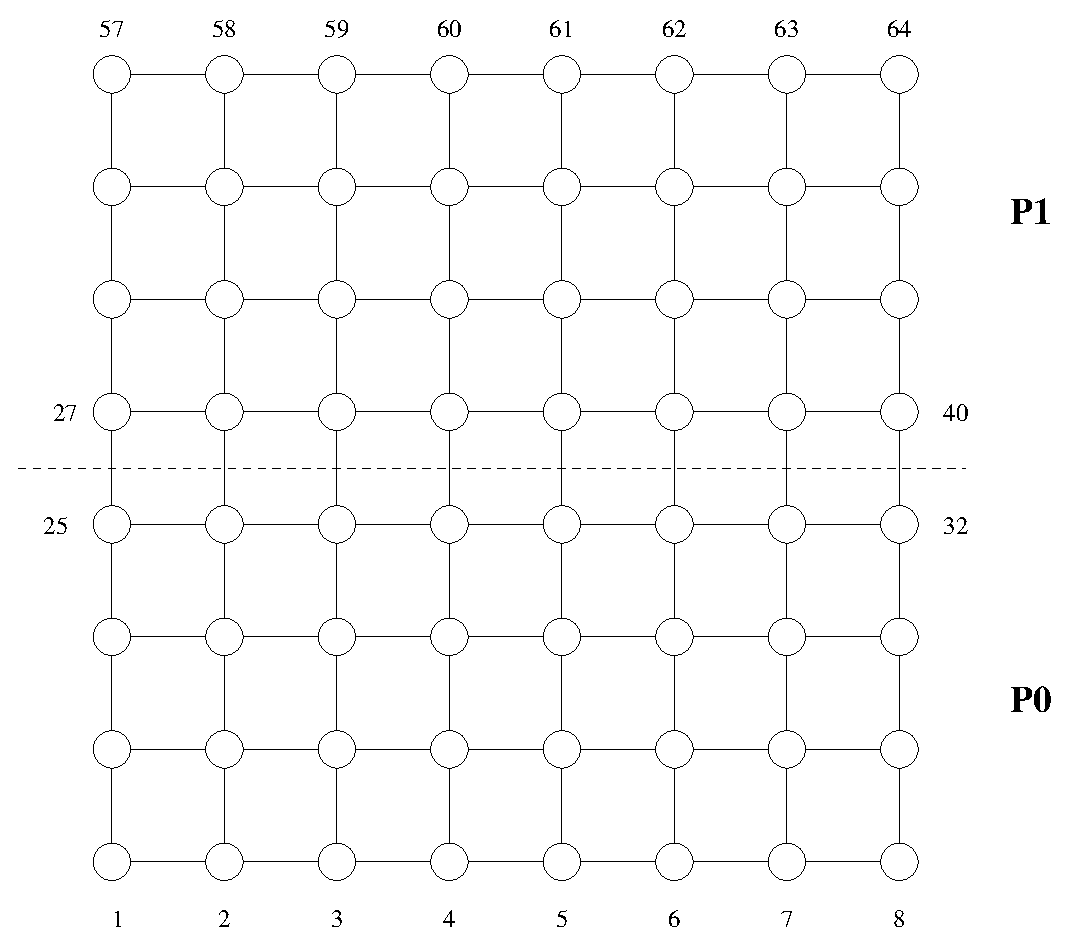
\includegraphics[scale=0.45]{figures/try8x8.eps}
\or
\rotatebox{-90}{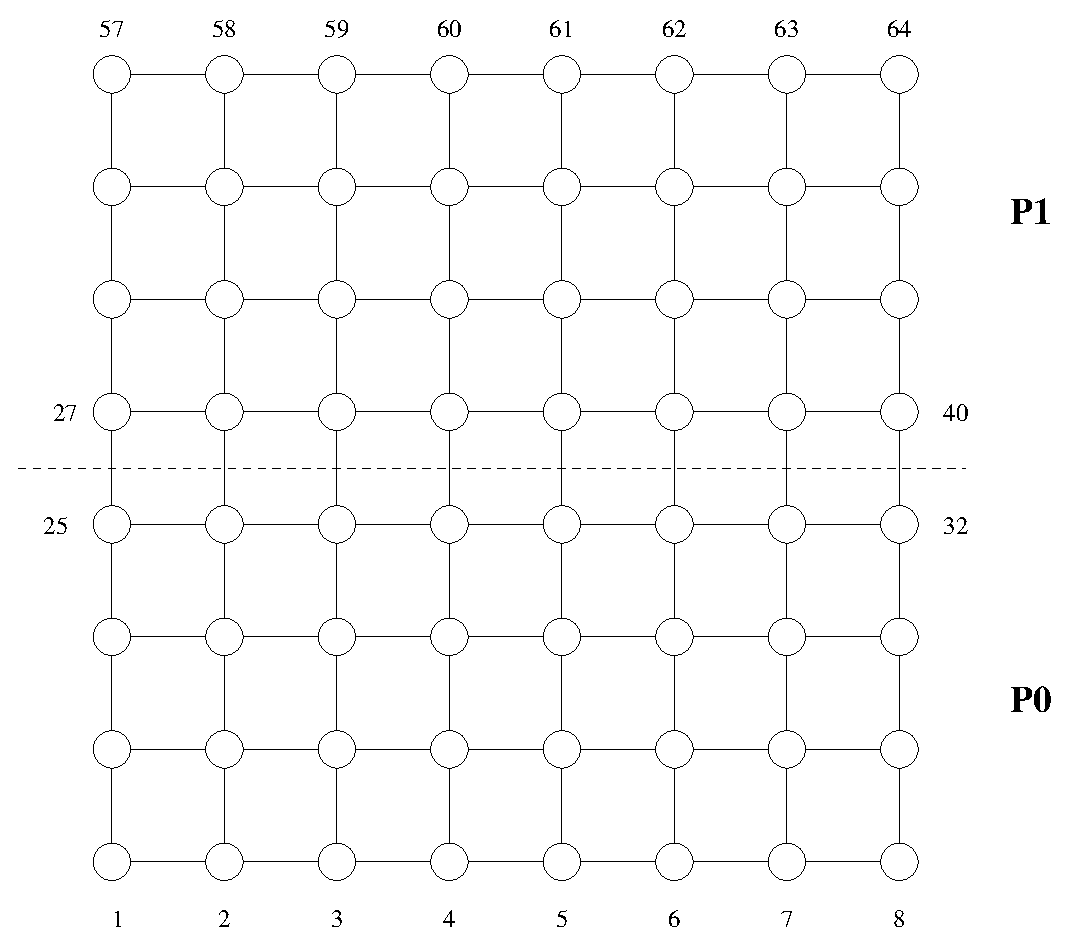
\includegraphics[scale=0.45]{figures/try8x8}}
\fi
\end{center}
\caption{Sample discretization mesh.\label{fig:try8x8}}
\end{figure}

{\par\noindent\large\bfseries Usage Example}
Consider the discretization mesh depicted in fig.~\ref{fig:try8x8},
partitioned among two processes as shown by the dashed line; the data
distribution is such that each process will own 32 entries in the
index space, with a halo made of 8 entries placed at local indices 33
through 40. If process 0 assigns an initial value of 1 to its entries
in the $x$ vector, and process 1 assigns a value of 2, then after a
call to \verb|psb_halo| the contents of the local vectors will be the
following: 
\begin{table}
\begin{center}
\small\begin{tabular}{rrr@{\hspace{6\tabcolsep}}rrr}
\multicolumn{3}{c}{Process  0}&
\multicolumn{3}{c}{Process  1}\\
  I  &   GLOB(I) & X(I)  &   I & GLOB(I) & X(I) \\
  1   &    1  &  1.0   &   1  &  33  &   2.0 \\ 
  2   &    2  &  1.0   &   2  &  34  &   2.0 \\
  3   &    3  &  1.0   &   3  &  35  &   2.0 \\
  4   &    4  &  1.0   &   4  &  36  &   2.0 \\
  5   &    5  &  1.0   &   5  &  37  &   2.0 \\
  6   &    6  &  1.0   &   6  &  38  &   2.0 \\
  7   &    7  &  1.0   &   7  &  39  &   2.0 \\
  8   &    8  &  1.0   &   8  &  40  &   2.0 \\
  9   &    9  &  1.0   &   9  &  41  &   2.0 \\
 10   &   10  &  1.0   &  10  &  42  &   2.0 \\
 11   &   11  &  1.0   &  11  &  43  &   2.0 \\
 12   &   12  &  1.0   &  12  &  44  &   2.0 \\
 13   &   13  &  1.0   &  13  &  45  &   2.0 \\
 14   &   14  &  1.0   &  14  &  46  &   2.0 \\
 15   &   15  &  1.0   &  15  &  47  &   2.0 \\
 16   &   16  &  1.0   &  16  &  48  &   2.0 \\
 17   &   17  &  1.0   &  17  &  49  &   2.0 \\
 18   &   18  &  1.0   &  18  &  50  &   2.0 \\
 19   &   19  &  1.0   &  19  &  51  &   2.0 \\
 20   &   20  &  1.0   &  20  &  52  &   2.0 \\ 
21   &   21  &  1.0   &  21  &  53  &   2.0 \\
22   &   22  &  1.0   &  22  &  54  &   2.0 \\
23   &   23  &  1.0   &  23  &  55  &   2.0 \\
24   &   24  &  1.0   &  24  &  56  &   2.0 \\
25   &   25  &  1.0   &  25  &  57  &   2.0 \\
26   &   26  &  1.0   &  26  &  58  &   2.0 \\
27   &   27  &  1.0   &  27  &  59  &   2.0 \\
28   &   28  &  1.0   &  28  &  60  &   2.0 \\
29   &   29  &  1.0   &  29  &  61  &   2.0 \\
30   &   30  &  1.0   &  30  &  62  &   2.0 \\
31   &   31  &  1.0   &  31  &  63  &   2.0 \\
32   &   32  &  1.0   &  32  &  64  &   2.0 \\
33   &   33  &  2.0   &  33  &  25  &   1.0 \\
34   &   34  &  2.0   &  34  &  26  &   1.0 \\
35   &   35  &  2.0   &  35  &  27  &   1.0 \\
36   &   36  &  2.0   &  36  &  28  &   1.0 \\
37   &   37  &  2.0   &  37  &  29  &   1.0 \\
38   &   38  &  2.0   &  38  &  30  &   1.0 \\
39   &   39  &  2.0   &  39  &  31  &   1.0 \\
40   &   40  &  2.0   &  40  &  32  &   1.0 \\
\end{tabular}
\end{center}
\end{table}

%%%%%%%%%%%%%%%%%%%%%%%%%%%%%%%%%%%%%%%%%%%%%%%%%%
%
%       OVERLAP UPDATE
%
%%%%%%%%%%%%%%%%%%%%%%%%%%%%%%%%%%%%%%%%%%%%%%%%%%


\clearpage\subsection*{psb\_ovrl --- Overlap Update}
\addcontentsline{toc}{subsection}{psb\_ovrl}    

These subroutines applies an overlap operator to the input vector:

\[ x \leftarrow Q x \]
where:
\begin{description}
\item[$x$] is the global dense submatrix $x$
\item[$Q$] is the overlap operator; it is the composition of two
operators $ P_a$ and $ P^{T}$. 
\end{description}

\begin{table}[h]
\begin{center}
\begin{tabular}{ll}
\hline
$x$ & {\bf Subroutine}\\
\hline
Short Precision Real & psb\_ovrl \\
Long Precision Real & psb\_ovrl \\
Short Precision Complex & psb\_ovrl \\
Long Precision Complex & psb\_ovrl \\
\hline
\end{tabular}
\end{center}
\caption{Data types\label{tab:f90ovrl}}
\end{table}

\begin{lstlisting}
call psb_ovrl(x, desc_a, info)
call psb_ovrl(x, desc_a, info, update=update_type, work=work)
\end{lstlisting} 

\begin{description}
\item[Type:] Synchronous.
\item[\bf On Entry]
\item[x] global dense matrix $x$.\\
Scope: {\bf local} \\
Type: {\bf required} \\
Intent: {\bf inout}.\\
Specified as:  a rank one or two array or an object of type \vdata\ 
containing numbers of type specified in
Table~\ref{tab:f90ovrl}.
\item[desc\_a] contains data structures for communications.\\
Scope: {\bf local} \\
Type: {\bf required}\\
Intent: {\bf in}.\\
Specified as: a structured data of type \descdata.
\item[update] Update operator. \\
\begin{description}
\item[update = psb\_none\_] Do nothing;
\item[update = psb\_add\_] Sum overlap entries, i.e. apply $P^T$;
\item[update = psb\_avg\_] Average overlap entries, i.e. apply $P_aP^T$;
%% \item[update = psb\_square\_root\_] square root update $\sqrt{P_a}$;
\end{description}
Scope: {\bf global} \\
Intent: {\bf in}.\\
Default: $update\_type = psb\_avg\_ $\\	
Scope: {\bf global} \\
Specified as: a integer variable.
\item[work] the work array. \\
Scope: {\bf local} \\
Type: {\bf optional}\\
Intent: {\bf inout}.\\
Specified as: a one dimensional array of the same type of $x$.

\item[\bf On Return] 
\item[x] global dense result matrix $x$.\\
Scope: {\bf local} \\
Type: {\bf required} \\
Intent: {\bf inout}.\\
Specified as: an  array of rank one or two
containing numbers of type specified in
Table~\ref{tab:f90ovrl}.
\item[info] Error code.\\
Scope: {\bf local} \\
Type: {\bf required} \\
Intent: {\bf out}.\\
An integer value; 0 means no error has been detected. 
\end{description}


{\par\noindent\large\bfseries Notes}
\begin{enumerate}
\item If there is no overlap in the data distribution associated with
  the descriptor, no operations are performed;
\item The operator $P^{T}$ performs the reduction sum of overlap
elements; it is a ``prolongation'' operator $P^T$ that
replicates overlap elements, accounting for the physical replication
of data;
\item The operator $P_a$ performs a scaling on the overlap elements by
the amount of replication; thus, when combined with the reduction
operator, it implements the average of replicated elements over all of
their instances. 
%% \item The square root update option makes it possible to applythe
%% following operator: 
%% \[ x\leftarrow \sqrt{P_a} P^{T} K^{-1} P \sqrt{P_a} x\]
%% In the case of a symmetric $K$, this preserves simmetry of the overall
%% preconditioner, which would otherwise be destroyed. 
\end{enumerate}
 
\begin{figure}[h] 
\begin{center}
\ifcase\pdfoutput
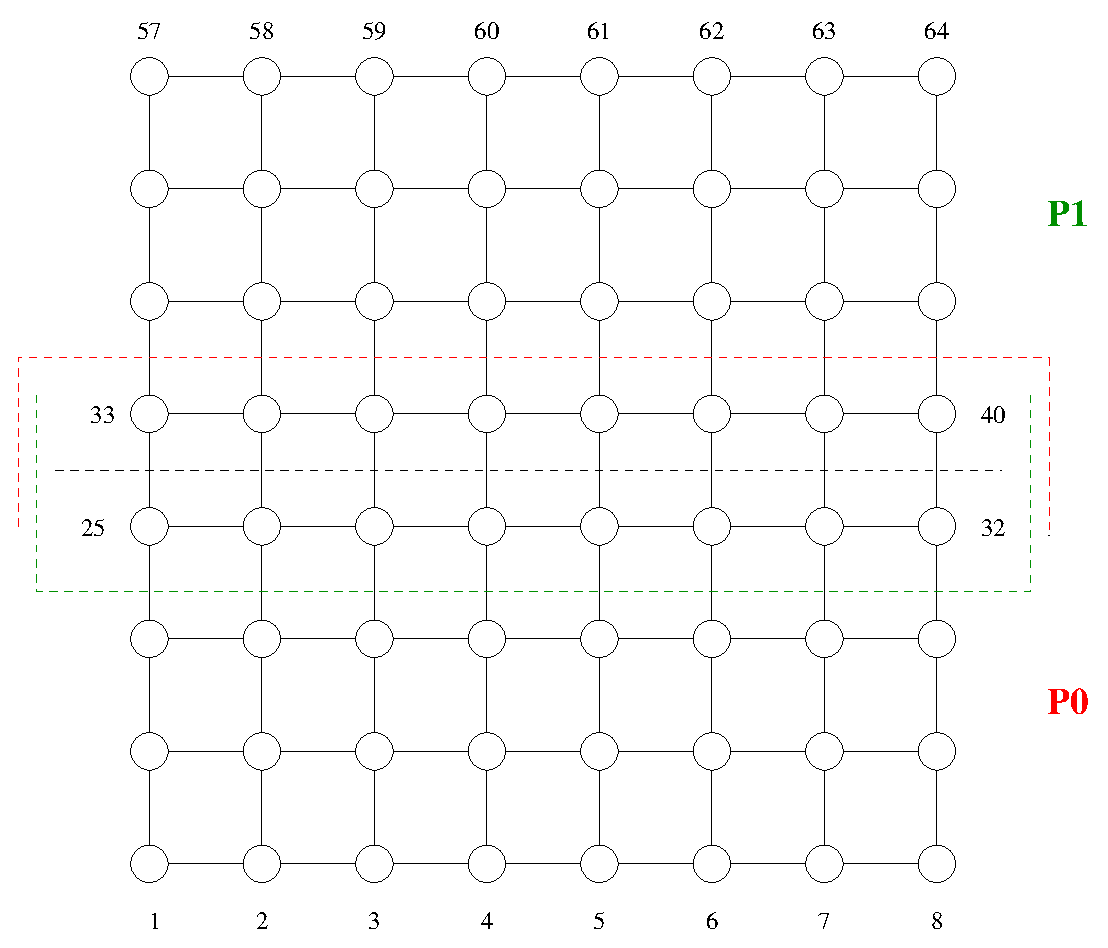
\includegraphics[scale=0.65]{figures/try8x8_ov.eps}
\or
\rotatebox{-90}{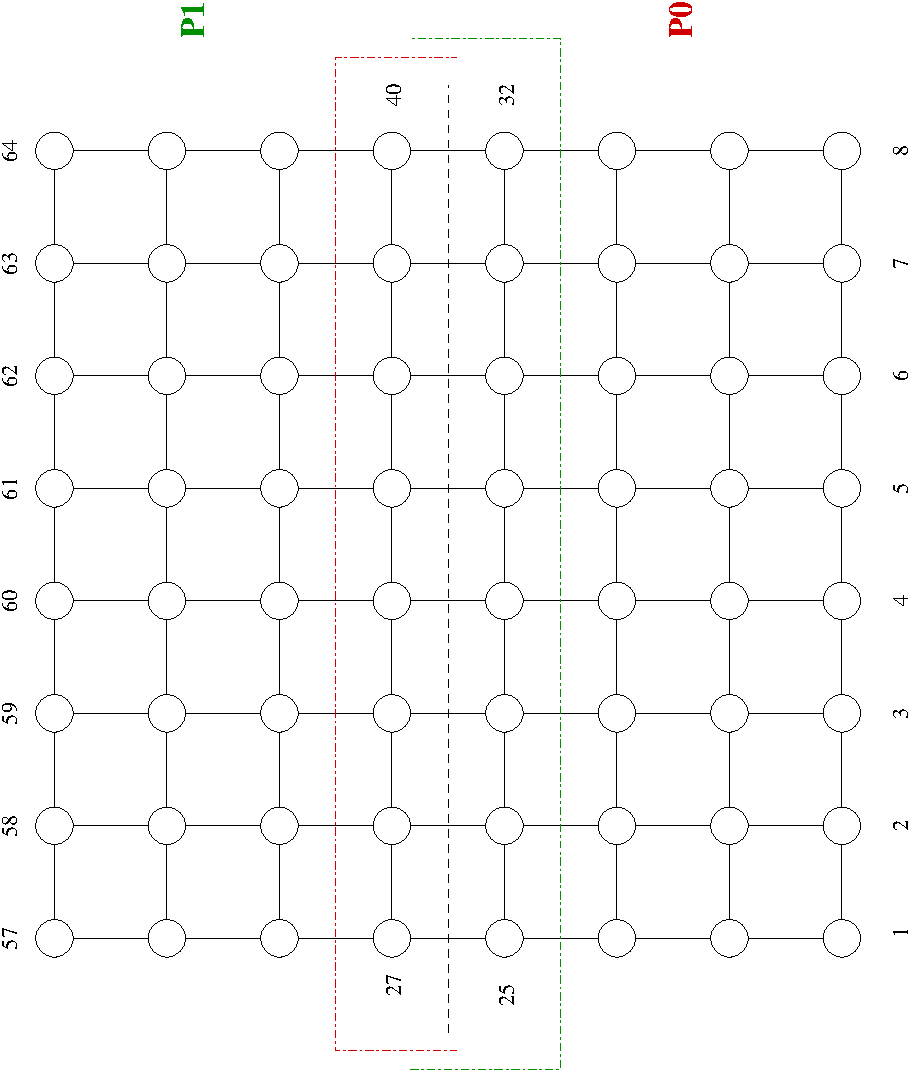
\includegraphics[scale=0.65]{figures/try8x8_ov}}
\fi
\end{center}
\caption{Sample discretization mesh.\label{fig:try8x8_ov}}
\end{figure}
{\par\noindent\large\bfseries Example of use}
Consider the discretization mesh depicted in fig.~\ref{fig:try8x8_ov},
partitioned among two processes as shown by the dashed lines, with an
overlap of 1 extra layer with respect to the partition of
fig.~\ref{fig:try8x8}; the data 
distribution is such that each process will own 40 entries in the
index space, with an overlap of 16  entries placed at local indices 25 
through 40; the halo will run from local index 41 through local index 48.. If process 0 assigns an initial value of 1 to its entries
in the $x$ vector, and process 1 assigns a value of 2, then after a
call to \verb|psb_ovrl| with \verb|psb_avg_| and a call to
\verb|psb_halo_| the contents of the local vectors will be the
following (showing a transition among the two subdomains)  

\begin{table}
\begin{center}
\footnotesize
\begin{tabular}{rrr@{\hspace{6\tabcolsep}}rrr}
\multicolumn{3}{c}{Process  0}&
\multicolumn{3}{c}{Process  1}\\
  I  &   GLOB(I) & X(I)  &   I & GLOB(I) & X(I) \\
  1   &    1  &  1.0   &   1  &  33  &   1.5 \\ 
  2   &    2  &  1.0   &   2  &  34  &   1.5 \\
  3   &    3  &  1.0   &   3  &  35  &   1.5 \\
  4   &    4  &  1.0   &   4  &  36  &   1.5 \\
  5   &    5  &  1.0   &   5  &  37  &   1.5 \\
  6   &    6  &  1.0   &   6  &  38  &   1.5 \\
  7   &    7  &  1.0   &   7  &  39  &   1.5 \\
  8   &    8  &  1.0   &   8  &  40  &   1.5 \\
  9   &    9  &  1.0   &   9  &  41  &   2.0 \\
 10   &   10  &  1.0   &  10  &  42  &   2.0 \\
 11   &   11  &  1.0   &  11  &  43  &   2.0 \\
 12   &   12  &  1.0   &  12  &  44  &   2.0 \\
 13   &   13  &  1.0   &  13  &  45  &   2.0 \\
 14   &   14  &  1.0   &  14  &  46  &   2.0 \\
 15   &   15  &  1.0   &  15  &  47  &   2.0 \\
 16   &   16  &  1.0   &  16  &  48  &   2.0 \\
 17   &   17  &  1.0   &  17  &  49  &   2.0 \\
 18   &   18  &  1.0   &  18  &  50  &   2.0 \\
 19   &   19  &  1.0   &  19  &  51  &   2.0 \\
 20   &   20  &  1.0   &  20  &  52  &   2.0 \\ 
 21   &   21  &  1.0   &  21  &  53  &   2.0 \\
 22   &   22  &  1.0   &  22  &  54  &   2.0 \\
 23   &   23  &  1.0   &  23  &  55  &   2.0 \\
 24   &   24  &  1.0   &  24  &  56  &   2.0 \\
 25   &   25  &  1.5   &  25  &  57  &   2.0 \\
 26   &   26  &  1.5   &  26  &  58  &   2.0 \\
 27   &   27  &  1.5   &  27  &  59  &   2.0 \\
 28   &   28  &  1.5   &  28  &  60  &   2.0 \\
 29   &   29  &  1.5   &  29  &  61  &   2.0 \\
 30   &   30  &  1.5   &  30  &  62  &   2.0 \\
 31   &   31  &  1.5   &  31  &  63  &   2.0 \\
 32   &   32  &  1.5   &  32  &  64  &   2.0 \\
 33   &   33  &  1.5   &  33  &  25  &   1.5 \\
 34   &   34  &  1.5   &  34  &  26  &   1.5 \\
 35   &   35  &  1.5   &  35  &  27  &   1.5 \\
 36   &   36  &  1.5   &  36  &  28  &   1.5 \\
 37   &   37  &  1.5   &  37  &  29  &   1.5 \\
 38   &   38  &  1.5   &  38  &  30  &   1.5 \\
 39   &   39  &  1.5   &  39  &  31  &   1.5 \\
 40   &   40  &  1.5   &  40  &  32  &   1.5 \\
 41   &   41  &  2.0   &  41  &  17  &   1.0 \\
 42   &   42  &  2.0   &  42  &  18  &   1.0 \\
 43   &   43  &  2.0   &  43  &  19  &   1.0 \\
 44   &   44  &  2.0   &  44  &  20  &   1.0 \\
 45   &   45  &  2.0   &  45  &  21  &   1.0 \\
 46   &   46  &  2.0   &  46  &  22  &   1.0 \\
 47   &   47  &  2.0   &  47  &  23  &   1.0 \\
 48   &   48  &  2.0   &  48  &  24  &   1.0 \\
\end{tabular}
\end{center}
\end{table}



%%%%%%%%%%%%%%%%%%%%%%%%%%%%%%%%%%%%%%%%%%%%%%%%%%
%
%      GATHER GLOBAL DENSE MATRIX
%
%%%%%%%%%%%%%%%%%%%%%%%%%%%%%%%%%%%%%%%%%%%%%%%%%%

\clearpage\subsection*{psb\_gather --- Gather Global Dense Matrix}
\addcontentsline{toc}{subsection}{psb\_gather}

These subroutines collect the portions of global dense matrix
distributed over all process into one single array stored on one
process.

\[ glob\_x \leftarrow collect(loc\_x_i) \]
where:
\begin{description}
\item[$glob\_x$] is the global submatrix $glob\_x_{1:m,1:n}$
\item[$loc\_x_i$] is the local portion of global dense matrix on
process $i$.
\item[$collect$] is the collect function.
\end{description}

\begin{table}[h]
\begin{center}
\begin{tabular}{ll}
\hline
$x_i, y$ & {\bf Subroutine}\\
\hline
Integer            & psb\_gather \\
Short Precision Real & psb\_gather \\
Long Precision Real & psb\_gather \\
Short Precision Complex & psb\_gather \\
Long Precision Complex & psb\_gather \\
\hline
\end{tabular}
\end{center}
\caption{Data types\label{tab:gather}}
\end{table}

\begin{lstlisting}
call psb_gather(glob_x, loc_x, desc_a, info, root)
call psb_gather(glob_x, loc_x, desc_a, info, root)
\end{lstlisting}

\begin{description}
\item[Type:] Synchronous.
\item[\bf On Entry]
\item[loc\_x] the local portion of global dense matrix
$glob\_x$. \\
Scope: {\bf local} \\
Type: {\bf required}\\
Intent: {\bf in}.\\
Specified as:  a rank one or two array or an object of type \vdata\ 
indicated in Table~\ref{tab:gather}.
\item[desc\_a] contains data structures for communications.\\
Scope: {\bf local} \\
Type: {\bf required}\\
Intent: {\bf in}.\\
Specified as: a structured data of type \descdata.
\item[root]  The process that holds the global copy. If $root=-1$ all
  the processes will have a copy of the global vector.\\
Scope: {\bf global} \\
Type: {\bf optional}\\
Intent: {\bf in}.\\
Specified as: an integer variable $-1\le root\le np-1$, default $-1$. 
%% \item[iglobx]  Row index to define a submatrix in glob\_x into which
%%   gather the local pieces.\\
%% Scope: {\bf global} \\
%% Type: {\bf optional}\\
%% Specified as: an integer variable $1\le ix\le matrix\_data(psb\_m\_)$. 
%% \item[jglobx]  Column index to define a submatrix in glob\_x into which
%%   gather the local pieces.\\
%% Scope: {\bf global} \\
%% Type: {\bf optional}\\
%% Specified as: an integer variable. 
%% \item[ilocx]  Row index to define a submatrix in loc\_x that has to
%%   be gathered into glob\_x.\\
%% Scope: {\bf local} \\
%% Type: {\bf optional}\\
%% Specified as: an integer variable. 
%% \item[jlocx]  Columns index to define a submatrix in loc\_x that has
%%   to be gathered into glob\_x.\\
%% Scope: {\bf global} \\
%% Type: {\bf optional}\\
%% Specified as: an integer variable.
%% \item[k]  The number of columns to gather.\\
%% Scope: {\bf global} \\
%% Type: {\bf optional}\\
%% Specified as: an integer variable. 
\item[\bf On Return] 
\item[glob\_x] The array where the local parts must be gathered.\\
Scope: {\bf global} \\
Type: {\bf required}\\
Intent: {\bf out}.\\
Specified as: a rank one or two array with the \verb|ALLOCATABLE| attribute.
\item[info] Error code.\\
Scope: {\bf local} \\
Type: {\bf required} \\
Intent: {\bf out}.\\
An integer value; 0 means no error has been detected. 
\end{description}

%%%%%%%%%%%%%%%%%%%%%%%%%%%%%%%%%%%%%%%%%%%%%%%%%%
%
%      SCATTER GLOBAL DENSE MATRIX
%
%%%%%%%%%%%%%%%%%%%%%%%%%%%%%%%%%%%%%%%%%%%%%%%%%%

\clearpage\subsection*{psb\_scatter --- Scatter Global Dense Matrix}
\addcontentsline{toc}{subsection}{psb\_scatter}

These subroutines scatters the portions of global dense matrix owned
by a process to all the processes in the processes grid.

\[ loc\_x_i \leftarrow scatter(glob\_x) \]
where:
\begin{description}
\item[$glob\_x$] is the global matrix $glob\_x_{1:m,1:n}$
\item[$loc\_x_i$] is the local portion of global dense matrix on
process $i$.
\item[$scatter$] is the scatter function.
\end{description}

\begin{table}[h]
\begin{center}
\begin{tabular}{ll}
\hline
$x_i, y$ & {\bf Subroutine}\\
\hline
Integer          & psb\_scatter \\
Short Precision Real & psb\_scatter \\
Long Precision Real & psb\_scatter \\
Short Precision Complex & psb\_scatter \\
Long Precision Complex & psb\_scatter \\
\hline
\end{tabular}
\end{center}
\caption{Data types\label{tab:scatter}}
\end{table}

\begin{lstlisting}
call psb_scatter(glob_x, loc_x, desc_a, info, root)
call psb_scatter(glob_x, loc_x, desc_a, info, root)
\end{lstlisting}

\begin{description}
\item[Type:] Synchronous.
\item[\bf On Entry]
\item[glob\_x] The array that must be scattered into local pieces.\\
Scope: {\bf global} \\
Type: {\bf required}\\
Intent: {\bf in}.\\
Specified as: a rank one or two array.
\item[desc\_a] contains data structures for communications.\\
Scope: {\bf local} \\
Type: {\bf required}\\
Intent: {\bf in}.\\
Specified as: a structured data of type \descdata.
\item[root]  The process that holds the global copy. If $root=-1$ all
  the processes have a copy of the global vector.\\
Scope: {\bf global} \\
Type: {\bf optional}\\
Intent: {\bf in}.\\
Specified as: an integer variable $-1\le root\le np-1$, default $-1$. 
%% \item[iglobx]  Row index to define a submatrix in glob\_x that has to
%%   be scattered into local pieces.\\
%% Scope: {\bf global} \\
%% Type: {\bf optional}\\
%% Specified as: an integer variable $1\le ix\le matrix\_data(psb\_m\_)$. 
%% \item[jglobx]  Column index to define a submatrix in glob\_x that has to
%%   be scattered into local pieces.\\
%% Scope: {\bf global} \\
%% Type: {\bf optional}\\
%% Specified as: an integer variable. 
%% \item[ilocx]  Row index to define a submatrix in loc\_x into which
%%   scatter the local piece of glob\_x.\\
%% Scope: {\bf local} \\
%% Type: {\bf optional}\\
%% Specified as: an integer variable. 
%% \item[jlocx]  Columns index to define a submatrix in loc\_x into which
%%   scatter the local piece of glob\_x.\\
%% Scope: {\bf global} \\
%% Type: {\bf optional}\\
%% Specified as: an integer variable.
%% \item[k]  The number of columns to scatter.\\
%% Scope: {\bf global} \\
%% Type: {\bf optional}\\
%% Specified as: an integer variable. 
\item[\bf On Return] 
\item[loc\_x] the local portion of global dense matrix
$glob\_x$. \\
Scope: {\bf local} \\
Type: {\bf required}\\
Intent: {\bf out}.\\
Specified as: a rank one or two array containing numbers of the type
indicated in Table~\ref{tab:scatter}.
\item[info] Error code.\\
Scope: {\bf local} \\
Type: {\bf required} \\
Intent: {\bf out}.\\
An integer value; 0 means no error has been detected. 
\end{description}

%%% Local Variables: 
%%% mode: latex
%%% TeX-master: "userguide"
%%% End: 

\section{Data management routines}
\label{sec:toolsrout}


%
%%   psb_cdall %%
%
\subsection*{psb\_cdall --- Allocates a communication descriptor}
\addcontentsline{toc}{subsection}{psb\_cdall}

\begin{verbatim}
call psb_cdall(icontxt, desc_a, info,mg=mg,parts=parts)
call psb_cdall(icontxt, desc_a, info,vg=vg,[mg=mg,flag=flag])
call psb_cdall(icontxt, desc_a, info,vl=vl,[nl=nl,globalcheck=.true.,lidx=lidx])
call psb_cdall(icontxt, desc_a, info,nl=nl)
call psb_cdall(icontxt, desc_a, info,mg=mg,repl=.true.)
\end{verbatim}

This subroutine initializes the communication descriptor associated
with an index space. One of the  optional arguments
\verb|parts|, \verb|vg|, \verb|vl|, \verb|nl|  or \verb|repl| 
must be specified, thereby choosing
the specific initialization strategy.
\begin{description}
\item[\bf  On Entry ]
\item[Type:] Synchronous.
\item[icontxt] the communication context.\\
Scope:{\bf global}.\\
Type:{\bf required}.\\
Intent: {\bf in}.\\
Specified as: an integer value.
\item[vg] Data allocation: each index $i\in \{1\dots mg\}$ is allocated
  to process $vg(i)$.\\
Scope:{\bf global}.\\
Type:{\bf optional}.\\
Intent: {\bf in}.\\
Specified as: an integer array. 
\item[flag] Specifies whether entries in $vg$ are zero- or one-based.\\
Scope:{\bf global}.\\
Type:{\bf optional}.\\
Intent: {\bf in}.\\
Specified as: an integer value $0,1$, default $0$.

\item[mg] the (global) number of rows of the problem.\\
Scope:{\bf global}.\\
Type:{\bf optional}.\\
Intent: {\bf in}.\\
Specified as: an integer value. It is required if \verb|parts| or
\verb|repl| is specified, it is optional if \verb|vg| is specified. 
\item[parts] the subroutine that defines the partitioning scheme.\\
Scope:{\bf global}.\\
Type:{\bf required}.\\
Specified as: a subroutine. 
\item[vl] Data allocation: the set of global indices 
  $vl(1:nl)$ belonging to the calling process. \\
Scope:{\bf local}.\\
Type:{\bf optional}.\\
Intent: {\bf in}.\\
Specified as: an integer array. 
\item[nl] Data allocation: in a generalized block-row distribution the
  number of indices belonging to the current process. \\
Scope:{\bf local}.\\
Type:{\bf optional}.\\
Intent: {\bf in}.\\
Specified as: an integer value. May be specified together with
\verb|vl|. 
\item[repl] Data allocation: build a replicated index space 
  (i.e. all processes own all indices).\\
Scope:{\bf global}.\\
Type:{\bf optional}.\\
Intent: {\bf in}.\\
Specified as: the logical value \verb|.true.|
\item[globalcheck] Data allocation: do global checks on the local
  index lists \verb|vl|\\
Scope:{\bf global}.\\
Type:{\bf optional}.\\
Intent: {\bf in}.\\
Specified as: a logical value, default: \verb|.true.|
\item[lidx] Data allocation: the set of local  indices 
  $lidx(1:nl)$ to be assigned to the global indices $vl$. \\
Scope:{\bf local}.\\
Type:{\bf optional}.\\
Intent: {\bf in}.\\
Specified as: an integer array. 
\end{description}

\begin{description}
\item[\bf On Return]
\item[desc\_a] the communication descriptor.\\
Scope:{\bf local}.\\
Type:{\bf required}.\\
Intent: {\bf out}.\\
Specified as: a structured data of type \descdata.
\item[info] Error code.\\
Scope: {\bf local} \\
Type: {\bf required} \\
Intent: {\bf out}.\\
An integer value; 0 means no error has been detected. 
\end{description}

{\par\noindent\large\bfseries Notes}
\begin{enumerate}
\item One of the optional arguments  \verb|parts|, \verb|vg|,
  \verb|vl|, \verb|nl|  or \verb|repl| must be specified, thereby choosing the
  initialization   strategy as follows:
\begin{description}
\item[parts] In this case we have a subroutine specifying the mapping
  between global indices and process/local index pairs. If this
  optional argument   is specified, then it is mandatory to 
  specify the argument \verb|mg| as well.  
  The subroutine must conform to the following interface: 
\begin{verbatim}
  interface 
     subroutine psb_parts(glob_index,mg,np,pv,nv)
       integer, intent (in)  :: glob_index,np,mg
       integer, intent (out) :: nv, pv(*)
     end subroutine psb_parts
  end interface
\end{verbatim}
  The input arguments are:
  \begin{description}
    \item[glob\_index] The global index to be mapped;
    \item[np] The number of processes in the mapping;
    \item[mg] The total number of global rows in the mapping;
  \end{description}
  The output arguments are:
  \begin{description}
    \item[nv] The number of entries in \verb|pv|;
    \item[pv] A vector containing the indices of the processes to
    which the global index should be assigend; each entry must satisfy
    $0\le pv(i) < np$; if $nv>1$ we have an index assigned to multiple
    processes, i.e. we have an overlap among the subdomains.
  \end{description}
\item[vg] In this case the association between an index and a process
  is specified via an integer vector  \verb|vg(1:mg)|; 
  each index $i \in \{1\dots mg\}$  is assigned to process $vg(i)$. 
  The vector \verb|vg| must be identical on all
  calling processes; its entries may have the ranges $(0\dots np-1)$
  or $(1\dots np)$ according to the value of \verb|flag|.  
  The size $mg$ may be  specified via the optional argument \verb|mg|;
  the default is to use the entire vector \verb|vg|, thus having
  \verb|mg=size(vg)|. 
\item[vl] In this case we are specifying the list of indices
  \verb|vl(1:nl)| assigned   to the current process; thus, the global
  problem size $mg$ is given by 
  the range of the aggregate of the individual vectors \verb|vl| specified
  in the calling processes. The size may be specified via the optional
  argument \verb|nl|; the default is to use the entire vector
  \verb|vl|, thus having   \verb|nl=size(vl)|.  
  If \verb|globalcheck=.true.|   the subroutine will check how many
  times  each entry in the global   index   space $(1\dots mg)$ is
  specified in the input lists   \verb|vl|, thus allowing for the
  presence of overlap in the input,   and checking for ``orphan''
  indices.    If \verb|globalcheck=.false.|, the subroutine will not
  check for   overlap, and may be significantly faster, but   the user
  is implicitly guaranteeing that there are neither orphan   nor
  overlap indices.  
\item[lidx] The optional argument \verb|lidx| is available for
  those cases in which the user has already established a
  global-to-local mapping; if it is specified, each  index in
  \verb|vl(i)| will be mapped to the corresponding local index
  \verb|lidx(i)|. When specifying the argument \verb|lidx| the user
  would also likely employ \verb|lidx| in calls to \verb|psb_cdins|
  and \verb|local| in calls to \verb|psb_spins| and \verb|psb_geins|;
  see also sec.~\ref{sec:usermaps}. 
\item[nl] If this argument is specified alone (i.e. without \verb|vl|)
  the  result is  a generalized row-block   distribution in which each
  process $I$ gets assigned a consecutive   chunk of $N_I=nl$ global
  indices. 
\item[repl] This arguments specifies to replicate all indices on
  all processes. This is a special purpose data allocation that is
  useful in the construction of some multilevel preconditioners.
\end{description}
\item On exit from this routine the descriptor is in the build
  state. 
\item Calling the routine with \verb|vg| or \verb|parts| implies that
  every process will scan the entire index space to figure out the
  local indices.
\item Overlapped indices are possible with both \verb|parts| and
  \verb|vl| invocations.
\item When the subroutine is invoked with \verb|vl| in
  conjunction with \verb|globalcheck=.true.|, it will perform a scan
  of the index   space to search for overlap or orphan indices.
\item When the subroutine is invoked with \verb|vl| in
  conjunction with \verb|globalcheck=.false.|, no index space scan
  will take place. Thus it is the responsibility of the user to make
  sure that the indices specified in \verb|vl| have neither orphans nor
  overlaps; if this assumption fails, results will be 
  unpredictable. 
\item Orphan and overlap indices are
  impossible by construction when the subroutine is invoked with
  \verb|nl| (alone),  or \verb|vg|.
\end{enumerate}


%
%%   psb_cdins %%
%
\clearpage\subsection*{psb\_cdins --- Communication descriptor insert routine}
\addcontentsline{toc}{subsection}{psb\_cdins}

\begin{verbatim}
call psb_cdins(nz, ia, ja, desc_a, info [,ila,jla])
call psb_cdins(nz,ja,desc,info[,jla,mask,lidx])
\end{verbatim}

This subroutine examines the edges of the graph associated with the
discretization mesh (and isomorphic to the sparsity pattern of a
linear system coefficient matrix), storing them as necessary into the
communication descriptor. In the first form the edges are specified as
pairs of indices $ia(i),ja(i)$; the starting index $ia(i)$ should
belong to the current process. 
In the second form only the remote indices $ja(i)$ are specified. 

\begin{description}
\item[Type:] Asynchronous.
\item[\bf On Entry]
\item[nz] the number of points being inserted.\\
Scope: {\bf local}.\\
Type: {\bf required}.\\
Intent: {\bf in}.\\
Specified as: an integer value.
\item[ia] the indices of the starting vertex of the edges  being inserted.\\
Scope: {\bf local}.\\
Type: {\bf required}.\\
Intent: {\bf in}.\\
Specified as: an integer array of length $nz$.
\item[ja]  the indices of the end vertex of the edges  being inserted.\\
Scope: {\bf local}.\\
Type: {\bf required}.\\
Intent: {\bf in}.\\
Specified as: an integer array of length $nz$.
\item[mask] Mask entries in \verb|ja|, they are inserted only when the
  corresponding \verb|mask| entries are \verb|.true.|\\
Scope: {\bf local}.\\
Type: {\bf optional}.\\
Intent: {\bf in}.\\
Specified as: a logical  array of length $nz$, default \verb|.true.|.
\item[lidx]  User defined local indices for \verb|ja|.\\
Scope: {\bf local}.\\
Type: {\bf optional}.\\
Intent: {\bf in}.\\
Specified as: an integer array of length $nz$.
%% \item[is] the row offset.\\
%% Scope:{\bf local}.\\
%% Type:{\bf optional}.\\a
%% Specified as: an integer value.
%% \item[js] the column offset.\\
%% Scope: {\bf local}.\\
%% Type: {\bf optional}.\\
%% Specified as: an integer value.
\end{description}

\begin{description}
\item[\bf On Return]
\item[desc\_a] the updated communication descriptor.\\
Scope:{\bf local}.\\
Type:{\bf required}.\\
Intent: {\bf inout}.\\
Specified as: a structured data of type \descdata.
\item[info] Error code.\\
Scope: {\bf local} \\
Type: {\bf required} \\
Intent: {\bf out}.\\
An integer value; 0 means no error has been detected. 
\item[ila] the local indices of the starting vertex of the edges  being inserted.\\
Scope: {\bf local}.\\
Type: {\bf optional}.\\
Intent: {\bf out}.\\
Specified as: an integer array of length $nz$.
\item[jla]  the local indices of the end vertex of the edges  being inserted.\\
Scope: {\bf local}.\\
Type: {\bf optional}.\\
Intent: {\bf out}.\\
Specified as: an integer array of length $nz$.

\end{description}
{\par\noindent\large\bfseries Notes}
\begin{enumerate}
\item This routine may only be called if the descriptor is in the
  build state;
\item  This routine automatically ignores edges that do not
insist on the  current process, i.e. edges for which neither the starting
nor the end vertex belong to the current process.
\item The second form of this routine will be useful when dealing with
  user-specified index mappings; see also~\ref{sec:usermaps}.
\end{enumerate}



%
%%   psb_cdasb %%
%
\clearpage\subsection*{psb\_cdasb --- Communication descriptor assembly routine}
\addcontentsline{toc}{subsection}{psb\_cdasb}

\begin{verbatim}
call psb_cdasb(desc_a, info)
\end{verbatim}

\begin{description}
\item[Type:] Synchronous.
\item[\bf On Entry]
\item[desc\_a] the communication descriptor.\\
Scope:{\bf local}.\\
Type:{\bf required}.\\
Intent: {\bf inout}.\\
Specified as: a structured data of type \descdata.
\end{description}

\begin{description}
\item[\bf On Return]
\item[desc\_a] the communication descriptor.\\
Scope:{\bf local}.\\
Type:{\bf required}.\\
Intent: {\bf inout}.\\
Specified as: a structured data of type \descdata.
\item[info] Error code.\\
Scope: {\bf local} \\
Type: {\bf required} \\
Intent: {\bf out}.\\
An integer value; 0 means no error has been detected. 
%\item[arg] 
\end{description}
{\par\noindent\large\bfseries Notes}
\begin{enumerate}
\item On exit from this routine the descriptor is in the assembled
  state. 
\end{enumerate}



%
%%   psb_cdcpy %%
%
\clearpage\subsection*{psb\_cdcpy --- Copies a communication descriptor}
\addcontentsline{toc}{subsection}{psb\_cdcpy}

\begin{verbatim}
call psb_cdcpy(desc_in, desc_out, info)
\end{verbatim}

\begin{description}
\item[Type:] Asynchronous.
\item[\bf On Entry]
\item[desc\_in] the communication descriptor.\\
Scope:{\bf local}.\\
Type:{\bf required}.\\
Intent: {\bf in}.\\
Specified as: a structured data of type \descdata.

\end{description}

\begin{description}
\item[\bf On Return]
\item[desc\_out] the communication descriptor copy.\\
Scope:{\bf local}.\\
Type:{\bf required}.\\
Intent: {\bf out}.\\
Specified as: a structured data of type \descdata.
\item[info] Error code.\\
Scope: {\bf local} \\
Type: {\bf required} \\
Intent: {\bf out}.\\
An integer value; 0 means no error has been detected. 
\end{description}


%
%%   psb_cdfree %%
%
\clearpage\subsection*{psb\_cdfree --- Frees a communication descriptor}
\addcontentsline{toc}{subsection}{psb\_cdfree}

\begin{verbatim}
call psb_cdfree(desc_a, info)
\end{verbatim}

\begin{description}
\item[Type:] Synchronous.
\item[\bf On Entry]
\item[desc\_a] the communication descriptor to be freed.\\
Scope:{\bf local}.\\
Type:{\bf required}.\\
Intent: {\bf inout}.\\
Specified as: a structured data of type \descdata.
\end{description}

\begin{description}
\item[\bf On Return]
\item[info] Error code.\\
Scope: {\bf local} \\
Type: {\bf required} \\
Intent: {\bf out}.\\
An integer value; 0 means no error has been detected. 
\end{description}



%
%%   psb_cdcpy %%
%
\clearpage\subsection*{psb\_cdbldext --- Build an extended  communication
  descriptor}
\addcontentsline{toc}{subsection}{psb\_cdbldext}

\begin{verbatim}
call psb_cdbldext(a,desc_a,nl,desc_out, info, extype)
\end{verbatim}

This subroutine builds an extended communication descriptor, based on
the input descriptor \verb|desc_a| and on the stencil specified
through the input sparse matrix \verb|a|. 
\begin{description}
\item[Type:] Synchronous.
\item[\bf On Entry]
\item[a] A sparse matrix
Scope:{\bf local}.\\
Type:{\bf required}.\\
Intent: {\bf in}.\\
Specified as: a structured data type.
\item[desc\_a] the communication descriptor.\\
Scope:{\bf local}.\\
Type:{\bf required}.\\
Intent: {\bf in}.\\
Specified as: a structured data of type \spdata.
\item[nl] the number of additional layers desired.\\
Scope:{\bf global}.\\
Type:{\bf required}.\\
Intent: {\bf in}.\\
Specified as: an integer value $nl\ge 0$. 
\item[extype] the kind of estension required.\\
Scope:{\bf global}.\\
Type:{\bf optional }.\\
Intent: {\bf in}.\\
Specified as: an integer value
\verb|psb_ovt_xhal_|, \verb|psb_ovt_asov_|, default: \verb|psb_ovt_xhal_|

\end{description}

\begin{description}
\item[\bf On Return]
\item[desc\_out] the extended communication descriptor.\\
Scope:{\bf local}.\\
Type:{\bf required}.\\
Intent: {\bf inout}.\\
Specified as: a structured data of type \descdata.
\item[info] Error code.\\
Scope: {\bf local} \\
Type: {\bf required} \\
Intent: {\bf out}.\\
An integer value; 0 means no error has been detected. 
\end{description}

{\par\noindent\large\bfseries Notes}
\begin{enumerate}
\item Specifying \verb|psb_ovt_xhal_| for the \verb|extype| argument
  the user will obtain a descriptor for a domain partition in which
  the additional layers are fetched as part of an (extended) halo;
  however the index-to-process mapping is identical to that of the
  base descriptor;
\item Specifying \verb|psb_ovt_asov_| for the \verb|extype| argument
  the user will obtain a descriptor with an overlapped decomposition:
  the additional layer is aggregated to  the local subdomain (and thus
  is an overlap), and a new halo extending beyond the last additional
  layer is formed. 
\end{enumerate}


%% %
%% %%   psb_cdren %%
%% %
%% \subsection*{psb\_cdren --- Applies a renumeration to a
%% communication descriptor}
%% \addcontentsline{toc}{subsection}{psb\_cdren}

%% \syntax{call psb\_cdren}{trans, iperm, desc\_a, info}

%% \begin{description}
%% \item[\bf On Entry]
%% \item[Type:] Asynchronous.
%% \item[trans] A character that specifies whether to permute $A$  or $A^T$.\\
%% Scope: {\bf local} \\
%% Type: {\bf required}\\
%% Specified as: a single character with value 'N' for $A$ or 'T' for $A^T$.\\
%% \item[iperm] An integer array containing permutation information.\\
%% Scope: {\bf local} \\
%% Type: {\bf required}\\
%% Specified as: an integer one-dimensional array.\\
%% \item[desc\_a] the communication descriptor.\\
%% Scope:{\bf local}.\\
%% Type:{\bf required}.\\
%% Specified as: a structured data of type \descdata.
%% \end{description}

%% \begin{description}
%% \item[\bf On Return]
%% \item[info] Error code.
%% Scope: {\bf local} \\
%% Type: {\bf required}\\
%% Specified as: an integer variable.
%% \end{description}




%
%%   psb_descprt %%
%
%% \subsection*{psb\_cdprt --- Prints a descriptor}
%%\addcontentsline{toc}{subsection}{psb\_cdprt}

%% \syntax{call psb\_cdprt}{iout, desc\_a, glob, short}

%% \begin{description}
%% \item[Type:] Asynchronous.
%% \item[\bf On Entry]
%% \item[iout] An integer that defines the output unit.
%% Scope: {\bf local} \\
%% Type: {\bf required}\\
%% Specified as: Integer scalar.\\
%% \item[desc\_a] The communication descriptor of type \descdata that
%%   must be printed.\\
%% Scope: {\bf local} \\
%% Type: {\bf required}\\
%% Specified as: a variable of type \descdata.\\
%% \end{description}

%% \begin{description}
%% \item[\bf On Return]
%% \item[glob] ??????
%% \item[short] ??????
%% \end{description}



%
%%   psb_spalloc %%
%
\clearpage\subsection*{psb\_spall --- Allocates a sparse matrix}
\addcontentsline{toc}{subsection}{psb\_spall}

\begin{verbatim}
call psb_spall(a, desc_a, info, nnz)
\end{verbatim}

\begin{description}
\item[Type:] Synchronous.
\item[\bf On Entry]
\item[desc\_a] the communication descriptor.\\
Scope:{\bf local}.\\
Type:{\bf required}.\\
Intent: {\bf in}.\\
Specified as: a structured data of type \descdata.
\item[nnz] An estimate of the number of nonzeroes in the local
  part of the assembled matrix.\\ 
Scope: {\bf global}.\\
Type: {\bf optional}.\\
Intent: {\bf in}.\\
Specified as: an integer value. 
\end{description}

\begin{description}
\item[\bf On Return]
\item[a] the matrix to be allocated.\\
Scope:{\bf local}\\
Type:{\bf required}\\
Intent: {\bf out}.\\
Specified as: a structured data of type \spdata.
\item[info] Error code.\\
Scope: {\bf local} \\
Type: {\bf required} \\
Intent: {\bf out}.\\
An integer value; 0 means no error has been detected. 
\end{description}
{\par\noindent\large\bfseries Notes}
\begin{enumerate}
\item On exit from this routine the sparse matrix  is in the build
  state.
\item The descriptor may be in either the build or assembled state.
\item Providing a good estimate for the number of nonzeroes $nnz$ in
  the assembled matrix may substantially improve performance in the
  matrix build phase, as it will reduce or eliminate the need for
  (potentially multiple) data reallocations. 
\end{enumerate}



%
%%   psb_spins %%
%
\clearpage\subsection*{psb\_spins --- Insert a cloud of elements into a sparse
  matrix}
\addcontentsline{toc}{subsection}{psb\_spins}

\begin{verbatim}
call psb_spins(nz, ia, ja, val, a, desc_a, info [,local])
\end{verbatim}

\begin{description}
\item[Type:] Asynchronous.
\item[\bf On Entry]
\item[nz] the number of elements to be inserted.\\
Scope:{\bf local}.\\
Type:{\bf required}.\\
Intent: {\bf in}.\\
Specified as: an integer scalar.
\item[ia] the row indices of the elements to be inserted.\\
Scope:{\bf local}.\\
Type:{\bf required}.\\
Intent: {\bf in}.\\
Specified as: an integer array of size $nz$.
\item[ja] the column indices of the elements to be inserted.\\
Scope:{\bf local}.\\
Type:{\bf required}.\\
Intent: {\bf in}.\\
Specified as: an integer array of size $nz$.
\item[val] the elements to be inserted.\\
Scope:{\bf local}.\\
Type:{\bf required}.\\
Intent: {\bf in}.\\
Specified as: an array of size $nz$. Must be of the same type and kind
of the coefficients  of the sparse matrix $a$.
\item[desc\_a] The communication descriptor.\\
Scope: {\bf local}. \\
Type: {\bf required}.\\
Intent: {\bf inout}.\\
Specified as: a variable of type \descdata.\\
\item[local] Whether the entries in the indices vectors \verb|ia|,
  \verb|ja| are already in local  numbering. \\
 Scope:{\bf local}.\\
 Type:{\bf optional}.\\
 Specified as: a logical value; default: \verb|.false.|.

%% \item[is] the starting row on matrix $a$.\\
%% Scope:{\bf local}.\\
%% Type:{\bf optional}.\\
%% Specified as: an integer vaule.
%% \item[js] the starting column on matrix $a$.\\
%% Scope:{\bf local}.\\
%% Type:{\bf optional}\\
%% Specified as: an integer value
\end{description}

\begin{description}
\item[\bf On Return]
\item[a] the matrix into which elements will be inserted.\\
Scope:{\bf local}\\
Type:{\bf required}\\
Intent: {\bf inout}.\\
Specified as: a structured data of type \spdata.
\item[desc\_a] The communication descriptor.\\
Scope: {\bf local}. \\
Type: {\bf required}.\\
Intent: {\bf inout}.\\
Specified as: a variable of type \descdata.\\
\item[info] Error code.\\
Scope: {\bf local} \\
Type: {\bf required} \\
Intent: {\bf out}.\\
An integer value; 0 means no error has been detected. 
\end{description}

{\par\noindent\large\bfseries Notes}
\begin{enumerate}
\item On entry to this routine the descriptor may be in either the
  build or assembled state.
\item On entry to this routine the sparse matrix may be in either the
  build or update state. 
\item If the descriptor is in the build state, then the sparse matrix
  must also be in the build state; the action of the routine is to
  (implicitly) call \verb|psb_cdins| to add entries to the sparsity
  pattern; each sparse matrix entry implicitly defines a graph edge,
  that is passed to the descriptor routine for the appropriate
  processing;
\item The coefficients to be inserted are represented by the ordered
  triples $ia(i),ja(i),val(i)$, for $i=1,\dots,nz$; these triples
  should belong to the current process, i.e. $ia(i)$ should be one of
  the local indices, but are otherwise arbitrary;
\item There is no
  requirement that a given row must be passed in its entirety to a
  single call to this routine: the buildup of a row may be split into
  as many calls as desired;
\item Coefficients from different rows   may also be mixed up freely
  in a single call, according to the application needs; 
\item Any coefficients from matrix rows not owned by the calling
  process are silently ignored;
\item If the descriptor is in the assembled state, then any entries in
  the sparse matrix that would generate additional communication
  requirements are  ignored; 
\item If the matrix is in the update state, any entries in positions
  that were not present in the original matrix are ignored. 
\end{enumerate}

%
%%   psb_spasb %%
%
\clearpage\subsection*{psb\_spasb --- Sparse matrix assembly routine}
\addcontentsline{toc}{subsection}{psb\_spasb}

\begin{verbatim}
call psb_spasb(a, desc_a, info, afmt, upd, dupl, mold)
\end{verbatim}

\begin{description}
\item[Type:] Synchronous.
\item[\bf On Entry]
\item[desc\_a] the communication descriptor.\\
Scope:{\bf local}.\\
Type:{\bf required}.\\
Intent: {\bf in}.\\
Specified as: a structured data of type \descdata.
\item[afmt] the storage format for the sparse matrix.\\
Scope: {\bf local}.\\
Type: {\bf optional}.\\
Intent: {\bf in}.\\
Specified as: an array of characters. Defalt:  'CSR'.
\item[upd] Provide for updates to the matrix coefficients.\\
Scope: {\bf global}.\\
Type: {\bf optional}.\\
Intent: {\bf in}.\\
Specified as: integer, possible values: \verb|psb_upd_srch_|, \verb|psb_upd_perm_|
\item[dupl] How to handle duplicate coefficients.\\
Scope: {\bf global}.\\
Type: {\bf optional}.\\
Intent: {\bf in}.\\
Specified as: integer, possible values: \verb|psb_dupl_ovwrt_|,
\verb|psb_dupl_add_|, \verb|psb_dupl_err_|.
\item[mold] The desired dynamic type for the internal matrix storage.\\
Scope: {\bf local}.\\
Type: {\bf optional}.\\
Intent: {\bf in}.\\
Specified as: an object of a class derived from \spbasedata. 
\end{description}

\begin{description}
\item[\bf On Return]
\item[a] the matrix to be assembled.\\
Scope:{\bf local}\\
Type:{\bf required}\\
Intent: {\bf inout}.\\
Specified as: a structured data of type \spdata.
\item[info] Error code.\\
Scope: {\bf local} \\
Type: {\bf required} \\
Intent: {\bf out}.\\
An integer value; 0 means no error has been detected. 
\end{description}

{\par\noindent\large\bfseries Notes}
\begin{enumerate}
\item On entry to this routine the descriptor must  be in  the
  assembled state, i.e. \verb|psb_cdasb| must already have been called.
\item The sparse matrix may be in either the build or update state;
\item Duplicate entries are detected and handled in both build and
  update state, with the exception of the error action that is only
  taken in the build state, i.e. on the first assembly; 
\item If the update choice is \verb|psb_upd_perm_|, then subsequent
  calls to \verb|psb_spins| to update the matrix must be arranged in
  such a way as to produce exactly the same sequence of coefficient
  values as encountered at the first assembly; 
\item The output storage format need not be the same on all
  processes; 
\item On exit from this routine the matrix is in the assembled state,
  and thus is suitable for the computational routines. 
\end{enumerate}



%% %
%% %%   psb_spcnv %%
%% %
%% \subsection*{psb\_spcnv --- Converts a sparse matrix storage
%% format}
%%\addcontentsline{toc}{subsection}{psb\_spcnv}

%% \syntax{call psb\_spcnv}{a, b, desc\_a, info}

%% \begin{description}
%% \item[\bf On Entry]
%% \item[a] the matrix to be converted.\\
%% Scope:{\bf local}\\
%% Type:{\bf required}\\
%% Specified as: a structured data of type \spdata.
%% \item[desc\_a] the communication descriptor.\\
%% Scope:{\bf local}.\\
%% Type:{\bf required}.\\
%% Specified as: a structured data of type \descdata.
%% \end{description}

%% \begin{description}
%% \item[\bf On Return]
%% \item[b] the converted matrix.\\
%% Scope:{\bf local}\\
%% Type:{\bf required}\\
%% Specified as: a structured data of type \spdata.
%% \item[info] Error code.
%% Scope: {\bf local} \\
%% Type: {\bf required}\\
%% Specified as: an integer variable.
%% \end{description}



%
%%   psb_spfree %%
%
\clearpage\subsection*{psb\_spfree --- Frees a sparse matrix}
\addcontentsline{toc}{subsection}{psb\_spfree}

\begin{verbatim}
call psb_spfree(a, desc_a, info)
\end{verbatim}

\begin{description}
\item[Type:] Synchronous.
\item[\bf On Entry]
\item[a] the matrix to be freed.\\
Scope:{\bf local}\\
Type:{\bf required}\\
Intent: {\bf inout}.\\
Specified as: a structured data of type \spdata.
\item[desc\_a] the communication descriptor.\\
Scope:{\bf local}.\\
Type:{\bf required}.\\
Intent: {\bf in}.\\
Specified as: a structured data of type \descdata.
\end{description}

\begin{description}
\item[\bf On Return]
\item[info] Error code.\\
Scope: {\bf local} \\
Type: {\bf required} \\
Intent: {\bf out}.\\
An integer value; 0 means no error has been detected. 
\end{description}




%
%%   psb_sprn %%
%
\clearpage\subsection*{psb\_sprn --- Reinit sparse matrix structure for psblas
  routines.}
\addcontentsline{toc}{subsection}{psb\_sprn}

\begin{verbatim}
call psb_sprn(a, decsc_a, info, clear)
\end{verbatim}

\begin{description}
\item[Type:] Synchronous.
\item[\bf On Entry]
\item[a] the matrix to be reinitialized.\\
Scope:{\bf local}\\
Type:{\bf required}\\
Intent: {\bf inout}.\\
Specified as: a structured data of type \spdata.
\item[desc\_a] the communication descriptor.\\
Scope:{\bf local}.\\
Type:{\bf required}.\\
Intent: {\bf in}.\\
Specified as: a structured data of type \descdata.
\item[clear] Choose whether to zero out matrix coefficients\\
Scope:{\bf local}.\\
Type:{\bf optional}.\\
Intent: {\bf in}.\\
Default: true.
\end{description}

\begin{description}
\item[\bf On Return]
\item[info] Error code.\\
Scope: {\bf local} \\
Type: {\bf required} \\
Intent: {\bf out}.\\
An integer value; 0 means no error has been detected. 
\end{description}
{\par\noindent\large\bfseries Notes}
\begin{enumerate}
\item On exit from this routine the sparse matrix is in the update
  state. 
\end{enumerate}
%
%%   psb_spupdate %%
%
%% \subsection*{psb\_spupdate --- Updates a sparse matrix.}
%%\addcontentsline{toc}{subsection}{psb\_spupdate}

%% \syntax{call psb\_spupdate}{a, ia, ja, blck, desc\_a, info, ix, jx, updflag}

%% \begin{description}
%% \item[\bf On Entry]
%% \end{description}

%% \begin{description}
%% \item[\bf On Return]
%% \end{description}
%% %
%% %%   psb_csrp %%
%% %
%% \subsection*{psb\_csrp --- Applies a right permutation to a sparse
%% matrix}
%%\addcontentsline{toc}{subsection}{psb\_csrp}

%% \syntax{call psb\_csrp}{trans, iperm, a, info}

%% \begin{description}
%% \item[\bf On Entry]
%% \item[trans] A character that specifies whether to permute $A$  or $A^T$.\\
%% Scope: {\bf local} \\
%% Type: {\bf required}\\
%% Specified as: a single character with value 'N' for $A$ or 'T' for $A^T$.\\
%% \item[iperm] An integer array containing permutation information.\\
%% Scope: {\bf local} \\
%% Type: {\bf required}\\
%% Specified as: an integer one-dimensional array.\\
%% \item[a] The sparse matrix to be permuted.\\
%% Scope: {\bf local} \\
%% Type: {\bf required}\\
%% Specified as: a \spdata variable.\\
%% \begin{description}
%% \item[\bf On Return]
%% \item[info] Error code.\\
%% Scope: {\bf local} \\
%% Type: {\bf required}\\
%% Specified as: Integer scalar.\\
%% \end{description}


%
%%   psb_alloc %%
%
\clearpage\subsection*{psb\_geall --- Allocates a dense matrix}
\addcontentsline{toc}{subsection}{psb\_geall}

\begin{verbatim}
call psb_geall(x, desc_a, info, n, lb)
\end{verbatim}

\begin{description}
\item[Type:] Synchronous.
\item[\bf On Entry]
\item[desc\_a] The communication descriptor.\\
Scope: {\bf local} \\
Type: {\bf required}\\
Intent: {\bf in}.\\
Specified as: a variable of type \descdata.\\
\item[n] The number of columns of the dense matrix to be allocated.\\
Scope: {\bf local} \\
Type: {\bf optional}\\
Intent: {\bf in}.\\
Specified as: Integer scalar, default $1$. It is not a valid argument  if $x$ is a
rank-1 array. 
\item[lb] The lower bound for the column index range of the dense matrix to be allocated.\\
Scope: {\bf local} \\
Type: {\bf optional}\\
Intent: {\bf in}.\\
Specified as: Integer scalar, default $1$. It is not a valid argument if $x$ is a
rank-1 array. 
\end{description}

\begin{description}
\item[\bf On Return]
\item[x] The dense matrix to be allocated.\\
Scope: {\bf local} \\
Type: {\bf required}\\
Intent: {\bf out}.\\
Specified as: a rank one or two array with the ALLOCATABLE  attribute
or an object of type \vdata, of type real, complex or integer.\\ 
\item[info] Error code.\\
Scope: {\bf local} \\
Type: {\bf required} \\
Intent: {\bf out}.\\
An integer value; 0 means no error has been detected. 
\end{description}


%
%%   psb_ins %%
%
\clearpage\subsection*{psb\_geins --- Dense matrix insertion routine}
\addcontentsline{toc}{subsection}{psb\_geins}

\begin{verbatim}
call psb_geins(m, irw, val, x, desc_a, info [,dupl,local])
\end{verbatim}

\begin{description}
\item[Type:] Asynchronous.
\item[\bf On Entry]
\item[m] Number of rows in $val$  to be inserted.\\
Scope:{\bf local}.\\
Type:{\bf required}.\\
Intent: {\bf in}.\\
Specified as: an integer value.
\item[irw] Indices of the rows to be inserted. Specifically, row $i$
  of $val$ will be inserted into the local row corresponding to the
  global row index $irw(i)$.
Scope:{\bf local}.\\
Type:{\bf required}.\\
Intent: {\bf in}.\\
Specified as: an integer array.
\item[val] the dense submatrix to be inserted.\\
Scope:{\bf local}.\\
Type:{\bf required}.\\
Intent: {\bf in}.\\
Specified as: a rank 1 or 2  array.
Specified as: an integer value.
\item[desc\_a] the communication descriptor.\\
Scope:{\bf local}.\\
Type:{\bf required}.\\
Intent: {\bf in}.\\
Specified as: a structured data of type \descdata.
\item[dupl] How to handle duplicate coefficients.\\
Scope: {\bf global}.\\
Type: {\bf optional}.\\
Intent: {\bf in}.\\
Specified as: integer, possible values: \verb|psb_dupl_ovwrt_|,
\verb|psb_dupl_add_|.
\item[local] Whether the entries in the index vector \verb|irw|,
   are already in local  numbering. \\
 Scope:{\bf local}.\\
 Type:{\bf optional}.\\
 Specified as: a logical value; default: \verb|.false.|.

\end{description}

\begin{description}
\item[\bf On Return]
\item[x] the output dense matrix.\\
Scope: {\bf local} \\
Type: {\bf required}\\
Intent: {\bf inout}.\\
Specified as:  a rank one or two array or an object of type \vdata, of
type real, complex or integer.\\ 
\item[info] Error code.\\
Scope: {\bf local} \\
Type: {\bf required} \\
Intent: {\bf out}.\\
An integer value; 0 means no error has been detected. 
\end{description}

{\par\noindent\large\bfseries Notes}
\begin{enumerate}
\item Dense vectors/matrices do not have an associated state;
\item Duplicate entries are either overwritten or added, there is no
  provision for raising an error condition. 
\end{enumerate}


%
%%   psb_asb %%
%
\clearpage\subsection*{psb\_geasb --- Assembly a dense matrix}
\addcontentsline{toc}{subsection}{psb\_geasb}

\begin{verbatim}
call psb_geasb(x, desc_a, info, mold)
\end{verbatim}

\begin{description}
\item[Type:] Synchronous.
\item[\bf On Entry]
\item[desc\_a] The communication descriptor.\\
Scope: {\bf local} \\
Type: {\bf required}\\
Intent: {\bf in}.\\
Specified as: a variable of type \descdata.\\
\item[mold] The desired dynamic type for the internal vector storage.\\
Scope: {\bf local}.\\
Type: {\bf optional}.\\
Intent: {\bf in}.\\
Specified as: an object of a class derived from \vbasedata; this is
only allowed when $x$ is of type \vdata.
\end{description}

\begin{description}
\item[\bf On Return]
\item[x] The dense matrix to be assembled.\\
Scope: {\bf local} \\
Type: {\bf required}\\
Intent: {\bf inout}.\\
Specified as: a rank one or two array with the ALLOCATABLE or an
object of type \vdata, of type real, complex or integer.\\
\item[info] Error code.\\
Scope: {\bf local} \\
Type: {\bf required} \\
Intent: {\bf out}.\\
An integer value; 0 means no error has been detected. 
\end{description}
%
%%   psb_free %%
%
\clearpage\subsection*{psb\_gefree --- Frees a dense matrix}
\addcontentsline{toc}{subsection}{psb\_gefree}

\begin{verbatim}
call psb_gefree(x, desc_a, info)
\end{verbatim}

\begin{description}
\item[Type:] Synchronous.
\item[\bf On Entry]
\item[x] The dense matrix to
  be freed.\\
Scope: {\bf local} \\
Type: {\bf required}\\
Intent: {\bf inout}.\\
Specified as: a rank one or two array with the ALLOCATABLE or an
object of type \vdata, of type real, complex or integer.\\

\item[desc\_a] The communication descriptor.\\
Scope: {\bf local} \\
Type: {\bf required}\\
Intent: {\bf in}.\\
Specified as: a variable of type \descdata.\\
\end{description}

\begin{description}
\item[\bf On Return]
\item[info] Error code.\\
Scope: {\bf local} \\
Type: {\bf required} \\
Intent: {\bf out}.\\
An integer value; 0 means no error has been detected. 
\end{description}


%
%%   psb_gelp %%
%
\clearpage\subsection*{psb\_gelp --- Applies a left permutation to a dense
  matrix}
\addcontentsline{toc}{subsection}{psb\_gelp}

\begin{verbatim}
call psb_gelp(trans, iperm, x, info)
\end{verbatim}

\begin{description}
\item[Type:] Asynchronous.
\item[\bf On Entry]
\item[trans] A character that specifies whether to permute $A$  or $A^T$.\\
Scope: {\bf local} \\
Type: {\bf required}\\
Intent: {\bf in}.\\
Specified as: a single character with value 'N' for $A$ or 'T' for $A^T$.\\
\item[iperm] An integer array containing permutation information.\\
Scope: {\bf local} \\
Type: {\bf required}\\
Intent: {\bf in}.\\
Specified as: an integer one-dimensional array.\\
\item[x] The dense matrix to be permuted.\\
Scope: {\bf local} \\
Type: {\bf required}\\
Intent: {\bf inout}.\\
Specified as: a one or two dimensional array.\\
\end{description}

\begin{description}
\item[\bf On Return]
\item[info] Error code.\\
Scope: {\bf local} \\
Type: {\bf required} \\
Intent: {\bf out}.\\
An integer value; 0 means no error has been detected. 
\end{description}


%
%%   psb_glob_to_loc %%
%
\clearpage\subsection*{psb\_glob\_to\_loc --- Global to local indices
  convertion}
\addcontentsline{toc}{subsection}{psb\_glob\_to\_loc}

\begin{verbatim}
call psb_glob_to_loc(x, y, desc_a, info, iact,owned)
call psb_glob_to_loc(x, desc_a, info, iact,owned)
\end{verbatim}

\begin{description}
\item[Type:] Asynchronous.
\item[\bf On Entry]
\item[x] An integer vector of indices to be converted.\\
Scope: {\bf local} \\
Type: {\bf required}\\
Intent: {\bf in, inout}.\\
Specified as: a rank one integer array.\\
\item[desc\_a] the communication descriptor.\\
Scope:{\bf local}.\\
Type:{\bf required}.\\
Intent: {\bf in}.\\
Specified as: a structured data of type \descdata.
\item[iact] specifies action to be taken in case of range errors. 
Scope: {\bf global} \\
Type: {\bf optional}\\
Intent: {\bf in}.\\
Specified as: a character variable  \verb|I|gnore, \verb|W|arning or
\verb|A|bort, default \verb|I|gnore.
\item[owned] Specfies valid range of input 
Scope: {\bf global} \\
Type: {\bf optional}\\
Intent: {\bf in}.\\
If true, then only indices strictly owned by the current process are
considered valid, if false then halo indices are also
accepted. Default: false. 
\end{description}

\begin{description}
\item[\bf On Return]
\item[x] If $y$ is not present,
  then $x$ is overwritten with the translated integer indices. 
Scope: {\bf global} \\
Type: {\bf required}\\
Intent: {\bf inout}.\\
Specified as: a rank one integer array.
\item[y] If $y$ is  present,
  then $y$ is overwritten with the translated integer indices, and $x$
  is left unchanged. 
Scope: {\bf global} \\
Type: {\bf optional}\\
Intent: {\bf out}.\\
Specified as: a rank one integer array.
\item[info] Error code.\\
Scope: {\bf local} \\
Type: {\bf required} \\
Intent: {\bf out}.\\
An integer value; 0 means no error has been detected. 
\end{description}

{\par\noindent\large\bfseries Notes}
\begin{enumerate}
\item If an input index is out of range, then the corresponding output
  index is set to a negative number;
\item The default \verb|I|gnore means that the negative output is the
  only action taken on an out-of-range input.
\end{enumerate}


\clearpage\subsection*{psb\_loc\_to\_glob --- Local to global indices
  conversion}
\addcontentsline{toc}{subsection}{psb\_loc\_to\_glob}

\begin{verbatim}
call psb_loc_to_glob(x, y, desc_a, info, iact)
call psb_loc_to_glob(x, desc_a, info, iact)
\end{verbatim}

\begin{description}
\item[Type:] Asynchronous.
\item[\bf On Entry]
\item[x] An integer vector of indices to be converted.\\
Scope: {\bf local} \\
Type: {\bf required}\\
Intent: {\bf in, inout}.\\
Specified as: a rank one integer array.\\
\item[desc\_a] the communication descriptor.\\
Scope:{\bf local}.\\
Type:{\bf required}.\\
Intent: {\bf in}.\\
Specified as: a structured data of type \descdata.
\item[iact] specifies action to be taken in case of range errors. 
Scope: {\bf global} \\
Type: {\bf optional}\\
Intent: {\bf in}.\\
Specified as: a character variable  \verb|I|gnore, \verb|W|arning or
\verb|A|bort, default \verb|I|gnore.
\end{description}

\begin{description}
\item[\bf On Return]
\item[x] If $y$ is not present,
  then $x$ is overwritten with the translated integer indices. 
Scope: {\bf global} \\
Type: {\bf required}\\
Intent: {\bf inout}.\\
Specified as: a rank one integer array.
\item[y] If $y$ is not present,
  then $y$ is overwritten with the translated integer indices, and $x$
  is left unchanged. 
Scope: {\bf global} \\
Type: {\bf optional}\\
Intent: {\bf out}.\\
Specified as: a rank one integer array.
\item[info] Error code.\\
Scope: {\bf local} \\
Type: {\bf required} \\
Intent: {\bf out}.\\
An integer value; 0 means no error has been detected. 
\end{description}



%
%%   psb_loc_to_glob %%
%
\clearpage\subsection*{psb\_is\_owned }
\addcontentsline{toc}{subsection}{psb\_is\_owned}

\begin{verbatim}
call psb_is_owned(x, desc_a)
\end{verbatim}

\begin{description}
\item[Type:] Asynchronous.
\item[\bf On Entry]
\item[x] Integer index.\\
Scope: {\bf local} \\
Type: {\bf required}\\
Intent: {\bf in}.\\
Specified as: a scalar integer.\\
\item[desc\_a] the communication descriptor.\\
Scope:{\bf local}.\\
Type:{\bf required}.\\
Intent: {\bf in}.\\
Specified as: a structured data of type \descdata.
\end{description}

\begin{description}
\item[\bf On Return]
\item[Function value] A logical mask which is true if 
  $x$ is  owned by the current process
Scope: {\bf local} \\
Type: {\bf required}\\
Intent: {\bf out}.\\
\end{description}


{\par\noindent\large\bfseries Notes}
\begin{enumerate}
\item This routine returns a \verb|.true.| value for an index
  that is strictly owned by the current process, excluding the halo
  indices
\end{enumerate}


\clearpage\subsection*{psb\_owned\_index }
\addcontentsline{toc}{subsection}{psb\_owned\_index}

\begin{verbatim}
call psb_owned_index(y, x, desc_a, info)
\end{verbatim}

\begin{description}
\item[Type:] Asynchronous.
\item[\bf On Entry]
\item[x] Integer indices.\\
Scope: {\bf local} \\
Type: {\bf required}\\
Intent: {\bf in, inout}.\\
Specified as: a scalar or a rank one integer array.\\
\item[desc\_a] the communication descriptor.\\
Scope:{\bf local}.\\
Type:{\bf required}.\\
Intent: {\bf in}.\\
Specified as: a structured data of type \descdata.
\item[iact] specifies action to be taken in case of range errors. 
Scope: {\bf global} \\
Type: {\bf optional}\\
Intent: {\bf in}.\\
Specified as: a character variable  \verb|I|gnore, \verb|W|arning or
\verb|A|bort, default \verb|I|gnore.
\end{description}

\begin{description}
\item[\bf On Return]
\item[y] A logical mask which is true for all corresponding entries of
  $x$ that are owned by the current process
Scope: {\bf local} \\
Type: {\bf required}\\
Intent: {\bf out}.\\
Specified as: a scalar or rank one logical array.
\item[info] Error code.\\
Scope: {\bf local} \\
Type: {\bf required} \\
Intent: {\bf out}.\\
An integer value; 0 means no error has been detected. 
\end{description}


{\par\noindent\large\bfseries Notes}
\begin{enumerate}
\item This routine returns a \verb|.true.| value for those indices
  that are strictly owned by the current process, excluding the halo
  indices
\end{enumerate}


\clearpage\subsection*{psb\_is\_local }
\addcontentsline{toc}{subsection}{psb\_is\_local}

\begin{verbatim}
call psb_is_local(x, desc_a)
\end{verbatim}

\begin{description}
\item[Type:] Asynchronous.
\item[\bf On Entry]
\item[x] Integer index.\\
Scope: {\bf local} \\
Type: {\bf required}\\
Intent: {\bf in}.\\
Specified as: a scalar integer.\\
\item[desc\_a] the communication descriptor.\\
Scope:{\bf local}.\\
Type:{\bf required}.\\
Intent: {\bf in}.\\
Specified as: a structured data of type \descdata.
\end{description}

\begin{description}
\item[\bf On Return]
\item[Function value] A logical mask which is true if 
  $x$ is  local to the current process
Scope: {\bf local} \\
Type: {\bf required}\\
Intent: {\bf out}.\\
\end{description}


{\par\noindent\large\bfseries Notes}
\begin{enumerate}
\item This routine returns a \verb|.true.| value for an index
  that is local to the current process, including the halo
  indices
\end{enumerate}

\clearpage\subsection*{psb\_local\_index }
\addcontentsline{toc}{subsection}{psb\_local\_index}

\begin{verbatim}
call psb_local_index(y, x, desc_a, info)
\end{verbatim}

\begin{description}
\item[Type:] Asynchronous.
\item[\bf On Entry]
\item[x] Integer indices.\\
Scope: {\bf local} \\
Type: {\bf required}\\
Intent: {\bf in, inout}.\\
Specified as: a scalar or a rank one integer array.\\
\item[desc\_a] the communication descriptor.\\
Scope:{\bf local}.\\
Type:{\bf required}.\\
Intent: {\bf in}.\\
Specified as: a structured data of type \descdata.
\item[iact] specifies action to be taken in case of range errors. 
Scope: {\bf global} \\
Type: {\bf optional}\\
Intent: {\bf in}.\\
Specified as: a character variable  \verb|I|gnore, \verb|W|arning or
\verb|A|bort, default \verb|I|gnore.
\end{description}

\begin{description}
\item[\bf On Return]
\item[y] A logical mask which is true for all corresponding entries of
  $x$ that are local to  the current process
Scope: {\bf local} \\
Type: {\bf required}\\
Intent: {\bf out}.\\
Specified as: a scalar or rank one logical array.
\item[info] Error code.\\
Scope: {\bf local} \\
Type: {\bf required} \\
Intent: {\bf out}.\\
An integer value; 0 means no error has been detected. 
\end{description}


{\par\noindent\large\bfseries Notes}
\begin{enumerate}
\item This routine returns a \verb|.true.| value for those indices
  that are local to  the current process, including the halo
  indices.
\end{enumerate}



%
%%   psb_ins %%
%
\clearpage\subsection*{psb\_get\_boundary --- Extract list of boundary elements}
\addcontentsline{toc}{subsection}{psb\_get\_boundary}

\begin{verbatim}
call psb_get_boundary(bndel, desc, info)
\end{verbatim}

\begin{description}
\item[Type:] Asynchronous.
\item[\bf On Entry]
\item[desc] the communication descriptor.\\
Scope:{\bf local}.\\
Type:{\bf required}.\\
Intent: {\bf in}.\\
Specified as: a structured data of type \descdata.
\end{description}

\begin{description}
\item[\bf On Return]
\item[bndel] The list of boundary elements on the calling process, in
  local numbering.\\
Scope: {\bf local} \\
Type: {\bf required}\\
Intent: {\bf out}.\\
Specified as: a rank one array with the ALLOCATABLE
attribute, of type integer.\\
\item[info] Error code.\\
Scope: {\bf local} \\
Type: {\bf required} \\
Intent: {\bf out}.\\
An integer value; 0 means no error has been detected. 
\end{description}

{\par\noindent\large\bfseries Notes}
\begin{enumerate}
\item If there are no boundary elements (i.e., if the local part of
  the connectivity graph is self-contained) the output vector is set
  to the ``not allocated'' state. 
\item Otherwise the size of \verb|bndel| will be exactly equal to the
  number of boundary elements. 
\end{enumerate}

\clearpage\subsection*{psb\_get\_overlap --- Extract list of overlap elements}
\addcontentsline{toc}{subsection}{psb\_get\_overlap}

\begin{verbatim}
call psb_get_overlap(ovrel, desc, info)
\end{verbatim}

\begin{description}
\item[Type:] Asynchronous.
\item[\bf On Entry]
\item[desc] the communication descriptor.\\
Scope:{\bf local}.\\
Type:{\bf required}.\\
Intent: {\bf in}.\\
Specified as: a structured data of type \descdata.
\end{description}

\begin{description}
\item[\bf On Return]
\item[ovrel] The list of overlap elements on the calling process, in
  local numbering.\\
Scope: {\bf local} \\
Type: {\bf required}\\
Intent: {\bf out}.\\
Specified as: a rank one array with the ALLOCATABLE
attribute, of type integer.\\
\item[info] Error code.\\
Scope: {\bf local} \\
Type: {\bf required} \\
Intent: {\bf out}.\\
An integer value; 0 means no error has been detected. 
\end{description}

{\par\noindent\large\bfseries Notes}
\begin{enumerate}
\item If there are no overlap elements the output vector is set
  to the ``not allocated'' state.  
\item Otherwise the size of \verb|ovrel| will be exactly equal to the
  number of overlap elements. 
\end{enumerate}



\clearpage\subsection*{psb\_sp\_getrow --- Extract row(s) from a sparse matrix}
\addcontentsline{toc}{subsection}{psb\_sp\_getrow}

\begin{verbatim}
call psb_sp_getrow(row, a, nz, ia, ja, val, info, &
              & append, nzin, lrw)
\end{verbatim}

\begin{description}
\item[Type:] Asynchronous.
\item[\bf On Entry]
\item[row] The (first) row to be extracted.\\
Scope:{\bf local}\\
Type:{\bf required}\\
Intent: {\bf in}.\\
Specified as: an integer $>0$.
\item[a] the matrix from  which to get rows.\\
Scope:{\bf local}\\
Type:{\bf required}\\
Intent: {\bf in}.\\
Specified as: a structured data of type \spdata.
\item[append] Whether to append or overwrite existing output.\\
Scope:{\bf local}\\
Type:{\bf optional}\\
Intent: {\bf in}.\\
Specified as: a logical value default: false (overwrite).
\item[nzin] Input size to be appended to.\\
Scope:{\bf local}\\
Type:{\bf optional}\\
Intent: {\bf in}.\\
Specified as: an integer $>0$. When append is true, specifies how many
entries in the output vectors are already filled. 
\item[lrw] The last  row to be extracted.\\
Scope:{\bf local}\\
Type:{\bf optional}\\
Intent: {\bf in}.\\
Specified as: an integer $>0$, default: $row$.

%% \item[is] the starting row on matrix $a$.\\
%% Scope:{\bf local}.\\
%% Type:{\bf optional}.\\
%% Specified as: an integer vaule.
%% \item[js] the starting column on matrix $a$.\\
%% Scope:{\bf local}.\\
%% Type:{\bf optional}\\
%% Specified as: an integer value
\end{description}

\begin{description}
\item[\bf On Return]
\item[nz] the number of elements returned by this call.\\
Scope:{\bf local}.\\
Type:{\bf required}.\\
Intent: {\bf out}.\\
Returned  as: an integer scalar.
\item[ia] the row indices.\\
Scope:{\bf local}.\\
Type:{\bf required}.\\
Intent: {\bf inout}.\\
Specified as: an integer array with the \verb|ALLOCATABLE| attribute.
\item[ja] the column indices of the elements to be inserted.\\
Scope:{\bf local}.\\
Type:{\bf required}.\\
Intent: {\bf inout}.\\
Specified as: an integer array with the \verb|ALLOCATABLE| attribute.
\item[val] the elements to be inserted.\\
Scope:{\bf local}.\\
Type:{\bf required}.\\
Intent: {\bf inout}.\\
Specified as: a real  array with the \verb|ALLOCATABLE| attribute.
\item[info] Error code.\\
Scope: {\bf local} \\
Type: {\bf required} \\
Intent: {\bf out}.\\
An integer value; 0 means no error has been detected. 
\end{description}

{\par\noindent\large\bfseries Notes}
\begin{enumerate}
\item The output $nz$ is always the size of the output generated by
  the current call; thus, if \verb|append=.true.|, the total output
  size will be $nzin+nz$, with the newly extracted coefficients stored in
  entries \verb|nzin+1:nzin+nz| of the array arguments;
\item When \verb|append=.true.|  the output arrays are reallocated as
  necessary;
\item The row and column indices are returned in the local numbering
  scheme; if the global numbering is desired, the user may employ the
  \verb|psb_loc_to_glob| routine on the output.
\end{enumerate}




\clearpage\subsection*{psb\_sizeof --- Memory occupation}
\addcontentsline{toc}{subsection}{psb\_sizeof}

This function computes the memory occupation of a PSBLAS object.


\begin{verbatim}
isz = psb_sizeof(a)
isz = psb_sizeof(desc_a)
isz = psb_sizeof(prec)
\end{verbatim}

\begin{description}
\item[Type:] Asynchronous.
\item[\bf On Entry]
\item[a] A sparse matrix
$A$. \\ 
Scope: {\bf local} \\
Type: {\bf required}\\
Intent: {\bf in}.\\
Specified as: a structured data of type \spdata.
\item[desc\_a] Communication descriptor.\\
Scope: {\bf local} \\
Type: {\bf required}\\
Intent: {\bf in}.\\
Specified as: a structured data of type \descdata.
\item[prec] 
Scope: {\bf local} \\
Type: {\bf required}\\
Intent: {\bf in}.\\
Specified as: a preconditioner data structure \precdata.
\item[\bf On Return] 
\item[Function value] The memory occupation of the object specified in
  the calling sequence, in bytes.\\
Scope: {\bf local} \\
Returned  as: an \verb|integer(psb_long_int_k_)| number.
\end{description}


\clearpage\subsection*{Sorting utilities}
\addcontentsline{toc}{subsection}{Sorting utilities}

{\par\noindent\large\bfseries psb\_msort --- Sorting by the Merge-sort
  algorithm}

{\par\noindent\large\bfseries psb\_qsort --- Sorting by the Quicksort
  algorithm}

{\par\noindent\large\bfseries psb\_hsort --- Sorting by the Heapsort  algorithm}
\begin{verbatim}
call psb_msort(x,ix,dir,flag)
call psb_qsort(x,ix,dir,flag)
call psb_hsort(x,ix,dir,flag)
\end{verbatim}

These  serial routines sort a sequence $X$ into ascending or
descending  order. The argument meaning is identical for the three
calls; the only difference is the algorithm used to accomplish the
task (see Usage Notes below). 
\begin{description}
\item[Type:] Asynchronous.
\item[\bf  On Entry ]
\item[x] The sequence to be sorted.\\
Type:{\bf required}.\\
Specified as: an integer, real or complex  array of rank 1.
\item[ix] A vector of indices.\\
Type:{\bf optional}.\\
Specified as: an integer array of (at least) the same size as $X$.
\item[dir] The desired ordering.\\
Type:{\bf optional}.\\
Specified as: an integer value: \begin{description}
\item[Integer and real data:] \verb|psb_sort_up_|,
\verb|psb_sort_down_|, \verb|psb_asort_up_|, \verb|psb_asort_down_|;
default \verb|psb_sort_up_|. 
\item[Complex data:] \verb|psb_lsort_up_|,
\verb|psb_lsort_down_|, \verb|psb_asort_up_|, \verb|psb_asort_down_|;
default \verb|psb_lsort_up_|. 
\end{description}
\item[flag] Whether to keep the original values in $IX$.\\
Type:{\bf optional}.\\
Specified as: an integer value \verb|psb_sort_ovw_idx_| or
\verb|psb_sort_keep_idx_|; default \verb|psb_sort_ovw_idx_|.

\end{description}

\begin{description}
\item[\bf On Return]
\item[x] The sequence of values, in the chosen ordering.\\ 
Type:{\bf required}.\\
Specified as: an integer, real or complex array of rank 1.
\item[ix] A vector of indices.\\
Type: {\bf Optional} \\
An integer array of rank 1, whose entries are moved to the same
position as the corresponding entries in $x$.
\end{description}

{\goodbreak\par\noindent\large\bfseries Notes}
\begin{enumerate}
\item For integer or real data the sorting can be performed in the up/down direction, on the
  natural or absolute values;
\item For  complex data the sorting can  be done in a lexicographic
  order (i.e.: sort on the real part with ties broken according to
  the imaginary part) or on the absolute values; 
\item The routines return the items in the chosen ordering; the
  output difference is the handling of  ties (i.e. items with an
  equal   value) in the original input. With the merge-sort algorithm
  ties are   preserved in the same relative order as they had in the
  original   sequence,  while this is not guaranteed for quicksort or
  heapsort; 
\item If $flag = psb\_sort\_ovw\_idx\_$ then the entries in $ix(1:n)$
  where $n$ is the size of $x$ are initialized to $ix(i) \leftarrow
  i$; thus, upon return from the subroutine, for each
  index $i$ we have in $ix(i)$ the position that the item $x(i)$
  occupied in the original data sequence;
\item If $flag = psb\_sort\_keep\_idx\_$  the routine will assume that
  the entries in $ix(:)$ have already been initialized by the user;
\item The three sorting algorithms have a similar $O(n \log n)$ expected
  running time; in the average case quicksort will be the
  fastest and merge-sort the slowest. However note that:
\begin{enumerate}
\item The worst case running time for quicksort is $O(n^2)$; the algorithm
  implemented here follows the well-known median-of-three heuristics,
  but the worst case may still apply;
\item The worst case running time for merge-sort and heap-sort is
  $O(n\log n)$  as the average case;
\item The merge-sort algorithm is implemented to take advantage of 
  subsequences that may be already in the desired ordering prior to
  the subroutine call; this situation is relatively common when
  dealing with groups of indices of sparse matrix entries, thus
  merge-sort is the preferred  choice when a sorting is needed
  by other routines in the library. 
\end{enumerate}
\end{enumerate}



%%% Local Variables: 
%%% mode: latex
%%% TeX-master: "userguide"
%%% End: 


\section{Parallel environment routines}
\label{sec:parenv}

\clearpage\subsection*{psb\_init --- Initializes PSBLAS parallel
  environment}
\addcontentsline{toc}{subsection}{psb\_init}

\begin{verbatim}
call psb_init(icontxt, np, basectxt, ids)
\end{verbatim}

This subroutine initializes the PSBLAS parallel environment, defining
a virtual parallel machine.
\begin{description}
\item[Type:] Synchronous.
\item[\bf  On Entry ]
\item[np] Number of processes in the PSBLAS virtual parallel machine.\\
Scope: {\bf global}.\\
Type: {\bf optional}.\\
Intent: {\bf in}.\\
Specified as: an integer value. \
Default: use all available processes.
\item[basectxt] the initial communication context. The new context
  will be defined from the processes participating in the initial one.\\
  Scope: {\bf global}.\\
Type: {\bf optional}.\\
Intent: {\bf in}.\\
Specified as: an integer value. \
Default: use MPI\_COMM\_WORLD.
\item[ids] Identities of the processes to use for the new context; the
  argument is ignored when \verb|np| is not specified. This allows the
  processes in the new environment to be in an order different from the
  original one.\\
  Scope: {\bf global}.\\
Type: {\bf optional}.\\
Intent: {\bf in}.\\
Specified as: an integer array. \
Default: use the indices $(0\dots np-1)$.  
\end{description}

\begin{description}
\item[\bf On Return]
\item[icontxt] the communication context identifying the virtual
  parallel machine. Note that this is always a duplicate of
  \verb|basectxt|, so that library communications are completely
  separated from other communication operations.\\
Scope: {\bf global}.\\
Type: {\bf required}.\\
Intent: {\bf out}.\\
Specified as: an integer variable.
\end{description}


{\par\noindent\large\bfseries Notes}
\begin{enumerate}
\item A call to this routine must precede any other PSBLAS call. 
\item It is an error to specify a value for $np$ greater than the
  number of processes available in the underlying base parallel
  environment. 
\end{enumerate}


\clearpage\subsection*{psb\_info --- Return information about  PSBLAS parallel
  environment}
\addcontentsline{toc}{subsection}{psb\_info}

\begin{verbatim}
call psb_info(icontxt, iam, np)
\end{verbatim}

This subroutine returns information about  the PSBLAS parallel environment, defining
a virtual parallel machine.
\begin{description}
\item[Type:] Asynchronous.
\item[\bf  On Entry ]
\item[icontxt] the communication context identifying the virtual
  parallel machine.\\
Scope: {\bf global}.\\
Type: {\bf required}.\\
Intent: {\bf in}.\\
Specified as: an integer variable.
\end{description}

\begin{description}
\item[\bf On Return]
\item[iam] Identifier of current  process in the PSBLAS virtual parallel machine.\\
Scope: {\bf local}.\\
Type: {\bf required}.\\
Intent: {\bf out}.\\
Specified as: an integer value. $-1 \le iam \le np-1$\
\item[np] Number of processes in the PSBLAS virtual parallel machine.\\
Scope: {\bf global}.\\
Type: {\bf required}.\\
Intent: {\bf out}.\\
Specified as: an integer variable. \
\end{description}


{\par\noindent\large\bfseries Notes}
\begin{enumerate}
\item For processes in the virtual parallel machine  the identifier
  will satisfy $0 \le iam \le np-1$;
\item If the user has requested on \verb|psb_init| a number of
  processes less than the total available in the parallel execution
  environment, the remaining processes will have on return $iam=-1$;
  the only call involving \verb|icontxt| that any such process may
  execute is  to \verb|psb_exit|. 
\end{enumerate}


\clearpage\subsection*{psb\_exit --- Exit from  PSBLAS parallel
  environment}
\addcontentsline{toc}{subsection}{psb\_exit}

\begin{verbatim}
call psb_exit(icontxt)
call psb_exit(icontxt,close)
\end{verbatim}

This subroutine exits from the  PSBLAS parallel virtual  machine.
\begin{description}
\item[Type:] Synchronous.
\item[\bf  On Entry ]
\item[icontxt] the communication context identifying the virtual
  parallel machine.\\
Scope: {\bf global}.\\
Type: {\bf required}.\\
Intent: {\bf in}.\\
Specified as: an integer variable.
\item[close] Whether to close all data structures related to the
  virtual parallel machine, besides those associated with icontxt.\\
Scope: {\bf global}.\\
Type: {\bf optional}.\\
Intent: {\bf in}.\\
Specified as: a logical  variable, default value: true.
\end{description}

{\par\noindent\large\bfseries Notes}
\begin{enumerate}
\item This routine may be called even if a previous call to
  \verb|psb_info| has returned with $iam=-1$; indeed, it it is the only
  routine that may be called with argument \verb|icontxt| in this
  situation.
\item A call to this routine with \verb|close=.true.| implies a call
  to \verb|MPI_Finalize|, after which no parallel routine may be called.
\item If the user whishes to use multiple communication contexts in the
  same program, or to enter and exit multiple times into the parallel
  environment, this routine may be called to 
  selectively close the contexts with \verb|close=.false.|, while on
  the last call it should be called with \verb|close=.true.| to
  shutdown in a clean way the entire parallel environment.
\end{enumerate}


\clearpage\subsection*{psb\_get\_mpicomm --- Get the MPI communicator}
\addcontentsline{toc}{subsection}{psb\_get\_mpicomm}

\begin{verbatim}
call psb_get_mpicomm(icontxt, icomm)
\end{verbatim}

This subroutine returns the MPI communicator associated with a PSBLAS context
\begin{description}
\item[Type:] Asynchronous.
\item[\bf  On Entry ]
\item[icontxt] the communication context identifying the virtual
  parallel machine.\\
Scope: {\bf global}.\\
Type: {\bf required}.\\
Intent: {\bf in}.\\
Specified as: an integer variable.
\end{description}

\begin{description}
\item[\bf On Return]
\item[icomm] The MPI communicator associated with the  PSBLAS virtual parallel machine.\\
Scope: {\bf global}.\\
Type: {\bf required}.\\
Intent: {\bf out}.\\
\end{description}


\clearpage\subsection*{psb\_get\_rank --- Get the MPI rank}
\addcontentsline{toc}{subsection}{psb\_get\_rank}

\begin{verbatim}
call psb_get_rank(rank, icontxt, id)
\end{verbatim}

This subroutine returns the MPI rank of the  PSBLAS process $id$
\begin{description}
\item[Type:] Asynchronous.
\item[\bf  On Entry ]
\item[icontxt] the communication context identifying the virtual
  parallel machine.\\
Scope: {\bf global}.\\
Type: {\bf required}.\\
Intent: {\bf in}.\\
Specified as: an integer variable.
\item[id] Identifier of a   process in the PSBLAS virtual parallel machine.\\
Scope: {\bf local}.\\
Type: {\bf required}.\\
Intent: {\bf in}.\\
Specified as: an integer value. $0 \le id \le np-1$\
\end{description}

\begin{description}
\item[\bf On Return]
\item[rank] The MPI rank associated with the  PSBLAS process $id$.\\
Scope: {\bf local}.\\
Type: {\bf required}.\\
Intent: {\bf out}.\\
\end{description}




\clearpage\subsection*{psb\_wtime --- Wall clock timing}
\addcontentsline{toc}{subsection}{psb\_wtime}

\begin{verbatim}
time = psb_wtime()
\end{verbatim}

This function returns a wall clock timer. The resolution of the timer
is dependent on the underlying parallel environment implementation.
\begin{description}
\item[Type:] Asynchronous.
\item[\bf  On Exit ]
\item[Function value] the elapsed time in seconds.\\
Returned  as: a  \verb|real(psb_dpk_)|  variable.
\end{description}


\clearpage\subsection*{psb\_barrier --- Sinchronization point  parallel
  environment}
\addcontentsline{toc}{subsection}{psb\_barrier}

\begin{verbatim}
call psb_barrier(icontxt)
\end{verbatim}

This subroutine acts as an explicit synchronization point for  the  PSBLAS
parallel virtual  machine. 
\begin{description}
\item[Type:] Synchronous.
\item[\bf  On Entry ]
\item[icontxt] the communication context identifying the virtual
  parallel machine.\\
Scope: {\bf global}.\\
Type: {\bf required}.\\
Intent: {\bf in}.\\
Specified as: an integer variable.
\end{description}


\clearpage\subsection*{psb\_abort --- Abort a computation}
\addcontentsline{toc}{subsection}{psb\_abort}

\begin{verbatim}
call psb_abort(icontxt)
\end{verbatim}

This subroutine aborts computation on the parallel virtual machine. 
\begin{description}
\item[Type:] Asynchronous.
\item[\bf  On Entry ]
\item[icontxt] the communication context identifying the virtual
  parallel machine.\\
Scope: {\bf global}.\\
Type: {\bf required}.\\
Intent: {\bf in}.\\
Specified as: an integer variable.
\end{description}





\clearpage\subsection*{psb\_bcast --- Broadcast data}
\addcontentsline{toc}{subsection}{psb\_bcast}

\begin{verbatim}
call psb_bcast(icontxt, dat, root)
\end{verbatim}

This subroutine implements a broadcast operation based on the
underlying communication library. 
\begin{description}
\item[Type:] Synchronous.
\item[\bf  On Entry ]
\item[icontxt] the communication context identifying the virtual
  parallel machine.\\
Scope: {\bf global}.\\
Type: {\bf required}.\\
Intent: {\bf in}.\\
Specified as: an integer variable.
\item[dat] On the root process, the data to be broadcast.\\
Scope: {\bf global}.\\
Type: {\bf required}.\\
Intent: {\bf inout}.\\
Specified as: an integer, real or complex variable, which may be a
scalar, or a rank 1 or 2 array, or a character or logical variable,
which may be a scalar or rank 1 array. \
Type, kind, rank and size must agree on all processes.
\item[root] Root process holding data to be broadcast.\\
Scope: {\bf global}.\\
Type: {\bf optional}.\\
Intent: {\bf in}.\\
Specified as: an integer value $0<= root <= np-1$, default 0 \
\end{description}


\begin{description}
\item[\bf On Return]
\item[dat] On processes other than  root, the data to be broadcast.\\
Scope: {\bf global}.\\
Type: {\bf required}.\\
Intent: {\bf inout}.\\
Specified as: an integer, real or complex variable, which may be a
scalar, or a rank 1 or 2 array, or a character or logical scalar. \
Type, kind, rank and size must agree on all processes.
\end{description}


\clearpage\subsection*{psb\_sum --- Global sum}
\addcontentsline{toc}{subsection}{psb\_sum}

\begin{verbatim}
call psb_sum(icontxt, dat, root)
\end{verbatim}

This subroutine implements a sum reduction  operation based on the
underlying communication library. 
\begin{description}
\item[Type:] Synchronous.
\item[\bf  On Entry ]
\item[icontxt] the communication context identifying the virtual
  parallel machine.\\
Scope: {\bf global}.\\
Type: {\bf required}.\\
Intent: {\bf in}.\\
Specified as: an integer variable.
\item[dat] The local contribution to the global sum.\\
Scope: {\bf global}.\\
Type: {\bf required}.\\
Intent: {\bf inout}.\\
Specified as: an integer, real or complex variable, which may be a
scalar, or a rank 1 or 2 array. \
Type, kind, rank and size must agree on all processes.
\item[root] Process to hold the final sum, or $-1$ to make it available
  on all processes.\\
Scope: {\bf global}.\\
Type: {\bf optional}.\\
Intent: {\bf in}.\\
Specified as: an integer value $-1<= root <= np-1$, default -1. \
\end{description}


\begin{description}
\item[\bf On Return]
\item[dat] On destination process(es), the result of the sum operation.\\
Scope: {\bf global}.\\
Type: {\bf required}.\\
Intent: {\bf inout}.\\
Specified as: an integer, real or complex variable, which may be a
scalar, or a rank 1 or 2 array. \\
Type, kind, rank and size must agree on all processes.
\end{description}

{\par\noindent\large\bfseries Notes}
\begin{enumerate}
\item The \verb|dat| argument is both input and output, and its
  value may be changed even on processes different from the final
  result destination.
\item The \verb|dat| argument may also be a long integer scalar.
\end{enumerate}



\clearpage\subsection*{psb\_max --- Global maximum}
\addcontentsline{toc}{subsection}{psb\_max}

\begin{verbatim}
call psb_max(icontxt, dat, root)
\end{verbatim}

This subroutine implements a maximum valuereduction
operation based on the underlying communication library. 
\begin{description}
\item[Type:] Synchronous.
\item[\bf  On Entry ]
\item[icontxt] the communication context identifying the virtual
  parallel machine.\\
Scope: {\bf global}.\\
Type: {\bf required}.\\
Intent: {\bf in}.\\
Specified as: an integer variable.
\item[dat] The local contribution to the global maximum.\\
Scope: {\bf local}.\\
Type: {\bf required}.\\
Intent: {\bf inout}.\\
Specified as: an integer or  real variable, which may be a
scalar, or a rank 1 or 2 array. \
Type, kind, rank and size must agree on all processes.
\item[root] Process to hold the final maximum, or $-1$ to make it available
  on all processes.\\
Scope: {\bf global}.\\
Type: {\bf optional}.\\
Intent: {\bf in}.\\
Specified as: an integer value $-1<= root <= np-1$, default -1. \\
\end{description}


\begin{description}
\item[\bf On Return]
\item[dat] On destination process(es), the result of the maximum operation.\\
Scope: {\bf global}.\\
Type: {\bf required}.\\
Intent: {\bf in}.\\
Specified as: an integer or  real variable, which may be a
scalar, or a rank 1 or 2 array. \
Type, kind, rank and size must agree on all processes.
\end{description}


{\par\noindent\large\bfseries Notes}
\begin{enumerate}
\item The \verb|dat| argument is both input and output, and its
  value may be changed even on processes different from the final
  result destination.
\item The \verb|dat| argument may also be a long integer scalar.
\end{enumerate}

\clearpage\subsection*{psb\_min --- Global minimum}
\addcontentsline{toc}{subsection}{psb\_min}

\begin{verbatim}
call psb_min(icontxt, dat, root)
\end{verbatim}

This subroutine implements a minimum value reduction
operation based on the underlying communication library. 
\begin{description}
\item[Type:] Synchronous.
\item[\bf  On Entry ]
\item[icontxt] the communication context identifying the virtual
  parallel machine.\\
Scope: {\bf global}.\\
Type: {\bf required}.\\
Intent: {\bf in}.\\
Specified as: an integer variable.
\item[dat] The local contribution to the global minimum.\\
Scope: {\bf local}.\\
Type: {\bf required}.\\
Intent: {\bf inout}.\\
Specified as: an integer  or real variable, which may be a
scalar, or a rank 1 or 2 array. \
Type, kind, rank and size must agree on all processes.
\item[root] Process to hold the final value, or $-1$ to make it available
  on all processes.\\
Scope: {\bf global}.\\
Type: {\bf optional}.\\
Intent: {\bf in}.\\
Specified as: an integer value $-1<= root <= np-1$, default -1. \\
\end{description}


\begin{description}
\item[\bf On Return]
\item[dat] On destination process(es), the result of the minimum operation.\\
Scope: {\bf global}.\\
Type: {\bf required}.\\
Intent: {\bf inout}.\\
Specified as: an integer  or  real variable, which may be a
scalar, or a rank 1 or 2 array. \\
Type, kind, rank and size must agree on all processes.
\end{description}


{\par\noindent\large\bfseries Notes}
\begin{enumerate}
\item The \verb|dat| argument is both input and output, and its
  value may be changed even on processes different from the final
  result destination.
\item The \verb|dat| argument may also be a long integer scalar.
\end{enumerate}

\clearpage\subsection*{psb\_amx --- Global maximum absolute value}
\addcontentsline{toc}{subsection}{psb\_amx}

\begin{verbatim}
call psb_amx(icontxt, dat, root)
\end{verbatim}

This subroutine implements a maximum absolute value reduction
operation based on the underlying communication library. 
\begin{description}
\item[Type:] Synchronous.
\item[\bf  On Entry ]
\item[icontxt] the communication context identifying the virtual
  parallel machine.\\
Scope: {\bf global}.\\
Type: {\bf required}.\\
Intent: {\bf in}.\\
Specified as: an integer variable.
\item[dat] The local contribution to the global maximum.\\
Scope: {\bf local}.\\
Type: {\bf required}.\\
Intent: {\bf inout}.\\
Specified as: an integer, real or complex variable, which may be a
scalar, or a rank 1 or 2 array. \
Type, kind, rank and size must agree on all processes.
\item[root] Process to hold the final value, or $-1$ to make it available
  on all processes.\\
Scope: {\bf global}.\\
Type: {\bf optional}.\\
Intent: {\bf in}.\\
Specified as: an integer value $-1<= root <= np-1$, default -1. \\
\end{description}


\begin{description}
\item[\bf On Return]
\item[dat] On destination process(es), the result of the maximum operation.\\
Scope: {\bf global}.\\
Type: {\bf required}.\\
Intent: {\bf inout}.\\
Specified as: an integer, real or complex variable, which may be a
scalar, or a rank 1 or 2 array. \
Type, kind, rank and size must agree on all processes.
\end{description}


{\par\noindent\large\bfseries Notes}
\begin{enumerate}
\item The \verb|dat| argument is both input and output, and its
  value may be changed even on processes different from the final
  result destination.
\item The \verb|dat| argument may also be a long integer scalar.
\end{enumerate}

\clearpage\subsection*{psb\_amn --- Global minimum absolute value}
\addcontentsline{toc}{subsection}{psb\_amn}

\begin{verbatim}
call psb_amn(icontxt, dat, root)
\end{verbatim}

This subroutine implements a minimum absolute value reduction
operation based on the underlying communication library. 
\begin{description}
\item[Type:] Synchronous.
\item[\bf  On Entry ]
\item[icontxt] the communication context identifying the virtual
  parallel machine.\\
Scope: {\bf global}.\\
Type: {\bf required}.\\
Intent: {\bf in}.\\
Specified as: an integer variable.
\item[dat] The local contribution to the global minimum.\\
Scope: {\bf local}.\\
Type: {\bf required}.\\
Intent: {\bf inout}.\\
Specified as: an integer, real or complex variable, which may be a
scalar, or a rank 1 or 2 array. \
Type, kind, rank and size must agree on all processes.
\item[root] Process to hold the final value, or $-1$ to make it available
  on all processes.\\
Scope: {\bf global}.\\
Type: {\bf optional}.\\
Intent: {\bf in}.\\
Specified as: an integer value $-1<= root <= np-1$, default -1. \\
\end{description}


\begin{description}
\item[\bf On Return]
\item[dat] On destination process(es), the result of the minimum operation.\\
Scope: {\bf global}.\\
Type: {\bf required}.\\
Intent: {\bf inout}.\\
Specified as: an integer, real or complex variable, which may be a
scalar, or a rank 1 or 2 array. \\
Type, kind, rank and size must agree on all processes.
\end{description}


{\par\noindent\large\bfseries Notes}
\begin{enumerate}
\item The \verb|dat| argument is both input and output, and its
  value may be changed even on processes different from the final
  result destination.
\item The \verb|dat| argument may also be a long integer scalar.
\end{enumerate}

\clearpage\subsection*{psb\_nrm2 --- Global 2-norm reduction}
\addcontentsline{toc}{subsection}{psb\_nrm2}

\begin{verbatim}
call psb_nrm2(icontxt, dat, root)
\end{verbatim}

This subroutine implements a 2-norm value reduction 
operation based on the underlying communication library. 
\begin{description}
\item[Type:] Synchronous.
\item[\bf  On Entry ]
\item[icontxt] the communication context identifying the virtual
  parallel machine.\\
Scope: {\bf global}.\\
Type: {\bf required}.\\
Intent: {\bf in}.\\
Specified as: an integer variable.
\item[dat] The local contribution to the global minimum.\\
Scope: {\bf local}.\\
Type: {\bf required}.\\
Intent: {\bf inout}.\\
Specified as: a real variable, which may be a
scalar, or a rank 1 array. \
Kind, rank and size must agree on all processes.
\item[root] Process to hold the final value, or $-1$ to make it available
  on all processes.\\
Scope: {\bf global}.\\
Type: {\bf optional}.\\
Intent: {\bf in}.\\
Specified as: an integer value $-1<= root <= np-1$, default -1. \\
\end{description}


\begin{description}
\item[\bf On Return]
\item[dat] On destination process(es), the result of the 2-norm reduction.\\
Scope: {\bf global}.\\
Type: {\bf required}.\\
Intent: {\bf inout}.\\
Specified as: a real variable, which may be a
scalar, or a rank 1 array. \\
Kind, rank and size must agree on all processes.
\end{description}


{\par\noindent\large\bfseries Notes}
\begin{enumerate}
\item This reduction is appropriate to compute the results of multiple
  (local) NRM2 operations at the same time. 
\item Denoting by $dat_i$ the value of the variable $dat$ on process
  $i$, the output $res$ is equivalent to the computation of
  \[ res = \sqrt{\sum_i dat_i^2},\]
  with care taken to avoid unnecessary overflow.
\item The \verb|dat| argument is both input and output, and its
  value may be changed even on processes different from the final
  result destination.
\end{enumerate}



\clearpage\subsection*{psb\_snd --- Send data}
\addcontentsline{toc}{subsection}{psb\_snd}

\begin{verbatim}
call psb_snd(icontxt, dat, dst, m)
\end{verbatim}

This subroutine sends a packet of data to a destination.
\begin{description}
\item[Type:] Synchronous: see usage notes. 
\item[\bf  On Entry ]
\item[icontxt] the communication context identifying the virtual
  parallel machine.\\
Scope: {\bf global}.\\
Type: {\bf required}.\\
Intent: {\bf in}.\\
Specified as: an integer variable.
\item[dat] The data to be sent.\\
Scope: {\bf local}.\\
Type: {\bf required}.\\
Intent: {\bf in}.\\
Specified as: an integer, real or complex variable, which may be a
scalar, or a rank 1 or 2 array, or a character or logical scalar. \
Type, kind and  rank must agree on sender and receiver process; if $m$ is
not specified, size must agree as well. 
\item[dst] Destination process.\\
Scope: {\bf global}.\\
Type: {\bf required}.\\
Intent: {\bf in}.\\
Specified as: an integer value $0<= dst <= np-1$. \\
\item[m] Number of rows.\\
Scope: {\bf global}.\\
Type: {\bf Optional}.\\
Intent: {\bf in}.\\
Specified as: an integer value $0<= m <= size(dat,1)$. \\
When $dat$ is a rank 2 array, specifies the number of rows to be sent
independently of the leading dimension $size(dat,1)$; must have the
same value on sending and receiving processes.
\end{description}


\begin{description}
\item[\bf On Return]
\end{description}

{\par\noindent\large\bfseries Notes}
\begin{enumerate}
\item This subroutine implies a synchronization, but only between the
  calling process and the destination  process $dst$.
\end{enumerate}


\clearpage\subsection*{psb\_rcv --- Receive data}
\addcontentsline{toc}{subsection}{psb\_rcv}

\begin{verbatim}
call psb_rcv(icontxt, dat, src, m)
\end{verbatim}

This subroutine receives a packet of data to a destination.
\begin{description}
\item[Type:] Synchronous: see usage notes.
\item[\bf  On Entry ]
\item[icontxt] the communication context identifying the virtual
  parallel machine.\\
Scope: {\bf global}.\\
Type: {\bf required}.\\
Intent: {\bf in}.\\
Specified as: an integer variable.
\item[src] Source process.\\
Scope: {\bf global}.\\
Type: {\bf required}.\\
Intent: {\bf in}.\\
Specified as: an integer value $0<= src <= np-1$. \\
\item[m] Number of rows.\\
Scope: {\bf global}.\\
Type: {\bf Optional}.\\
Intent: {\bf in}.\\
Specified as: an integer value $0<= m <= size(dat,1)$. \\
When $dat$ is a rank 2 array, specifies the number of rows to be sent
independently of the leading dimension $size(dat,1)$; must have the
same value on sending and receiving processes.
\end{description}


\begin{description}
\item[\bf On Return]
\item[dat] The data to be received.\\
Scope: {\bf local}.\\
Type: {\bf required}.\\
Intent: {\bf inout}.\\
Specified as: an integer, real or complex variable, which may be a
scalar, or a rank 1 or 2 array, or a character or logical scalar. \
Type, kind and  rank must agree on sender and receiver process; if $m$ is
not specified, size must agree as well. 
\end{description}

{\par\noindent\large\bfseries Notes}
\begin{enumerate}
\item This subroutine implies a synchronization, but only between the
  calling process and the source  process $src$.
\end{enumerate}



\section{Error handling}

The PSBLAS library error handling policy has been completely rewritten
in version 2.0. The idea behind the design of this new error handling
strategy is to keep error messages on a stack allowing the user to
trace back up to the point where the first error message has been
generated. Every routine in the PSBLAS-2.0 library has, as last
non-optional argument, an integer \verb|info| variable; whenever,
inside the routine, an error is detected, this variable is set to a
value corresponding to a specific error code. Then this error code is
also pushed on the error stack and then either control is returned to
the caller routine or the execution is aborted, depending on the users
choice. At the time when the execution is aborted, an error message is
printed on standard output with a level of verbosity than can be
chosen by the user. If the execution is not aborted, then, the caller
routine checks the value returned in the \verb|info| variable and, if
not zero, an error condition is raised. This process continues on all the
levels of nested calls until the level where the user decides to abort
the program execution.

Figure~\ref{fig:routerr} shows the layout of a generic \verb|psb_foo|
routine with respect to the PSBLAS-2.0 error handling policy. It is
possible to see how, whenever an error condition is detected, the
\verb|info| variable is set to the corresponding error code which is,
then, pushed on top of the stack by means of the
\verb|psb_errpush|. An error condition may be directly detected inside
a routine or indirectly checking the error code returned returned by a
called routine. Whenever an error is encountered, after it has been
pushed on stack, the program execution skips to a point where the
error condition is handled; the error condition is handled either by
returning control to the caller routine or by calling the
\verb|psb\_error| routine which prints the content of the error stack
and aborts the program execution, according to the choice made by the
user with \verb|psb_set_erraction|. The default is to print the error
and terminate the program, but the user may choose to handle the error
explicitly. 

\begin{figure}[h!]
  \begin{Sbox}
    \begin{minipage}[tl]{0.95\textwidth}
\small
\begin{lstlisting}
subroutine psb_foo(some args, info)
   ...
   if(error detected) then
      info=errcode1
      call psb_errpush('psb_foo', errcode1)
      goto 9999
   end if
   ...
   call psb_bar(some args, info)
   if(info .ne. zero) then
      info=errcode2
      call psb_errpush('psb_foo', errcode2)
      goto 9999
   end if
   ...
9999 continue
   if (err_act .eq. act_abort) then
     call psb_error(icontxt)
     return
   else
     return
   end if

end subroutine psb_foo
\end{lstlisting}
    \end{minipage}
  \end{Sbox}
  \setlength{\fboxsep}{8pt}
  \begin{center}
    \fbox{\TheSbox}
  \end{center}
  \caption{\label{fig:routerr}The layout of a generic \texttt{psb\_foo}
  routine with respect to PSBLAS-2.0 error handling policy.}
\end{figure}




Figure~\ref{fig:errormsg} reports a sample error message generated by
the PSBLAS-2.0 library. This error has been generated by the fact that
the user has chosen the invalid ``FOO'' storage format to represent
the sparse matrix. From this error message it is possible to see that
the error has been detected inside the \verb|psb_cest| subroutine
called by \verb|psb_spasb| ... by process 0 (i.e. the root process).


\begin{figure}[h!]
  \begin{Sbox}
    \begin{minipage}[tl]{0.95\textwidth}
\begin{verbatim}
==========================================================
Process: 0.  PSBLAS Error (4010) in subroutine: df_sample           
Error from call to subroutine mat dist            
==========================================================
Process: 0.  PSBLAS Error (4010) in subroutine: mat_distv           
Error from call to subroutine psb_spasb           
==========================================================
Process: 0.  PSBLAS Error (4010) in subroutine: psb_spasb           
Error from call to subroutine psb_cest            
==========================================================
Process: 0.  PSBLAS Error (136) in subroutine: psb_cest            
Format FOO is unknown
==========================================================
Aborting...
\end{verbatim}
    \end{minipage}
  \end{Sbox}
  \setlength{\fboxsep}{8pt}
  \begin{center}
    \fbox{\TheSbox}
  \end{center}
  \caption{\label{fig:errormsg}A sample PSBLAS-2.0 error
    message. Process 0 detected an error condition inside the {\textrm
    psb\_cest} subroutine}
\end{figure}


\clearpage\subroutine{psb\_errpush}{Pushes an error code onto the error
  stack}

\begin{lstlisting}
call psb_errpush(err_c, r_name, i_err, a_err)
\end{lstlisting}

\begin{description}
\item[Type:] Asynchronous.
\item[\bf On Entry]
\item[err\_c] the error code\\
Scope: {\bf local} \\
Type: {\bf required}\\
Intent: {\bf in}.\\
Specified as: an integer.
\item[r\_name] the soutine where the error has been caught.\\
Scope: {\bf local} \\
Type: {\bf required}\\
Intent: {\bf in}.\\
Specified as: a string.\\
\item[i\_err] addional info for error code\\
Scope: {\bf local} \\
Type: {\bf optional}\\
Specified as: an integer array\\
\item[a\_err] addional info for error code\\
Scope: {\bf local} \\
Type: {\bf optional}\\
Specified as: a string.\\
\end{description}

\clearpage\subroutine{psb\_error}{Prints the error stack content and aborts
  execution}

\begin{lstlisting}
call psb_error(icontxt)
\end{lstlisting}

\begin{description}
\item[Type:] Asynchronous.
\item[\bf On Entry]
\item[icontxt] the communication context.\\
Scope: {\bf global} \\
Type: {\bf optional}\\
Intent: {\bf in}.\\
Specified as: an integer.
\end{description}



\clearpage\subroutine{psb\_set\_errverbosity}{Sets the verbosity of error
  messages.}

\begin{lstlisting}
call psb_set_errverbosity(v)
\end{lstlisting}

\begin{description}
\item[Type:] Asynchronous.
\item[\bf On Entry]
\item[v] the verbosity level\\
Scope: {\bf global}\\
Type: {\bf required}\\
Intent: {\bf in}.\\
Specified as: an integer.
\end{description}

\clearpage\subroutine{psb\_set\_erraction}{Set the type of action to be
  taken  upon error condition.}


\begin{lstlisting}
call psb_set_erraction(err_act)
\end{lstlisting}

\begin{description}
\item[Type:] Asynchronous.
\item[\bf On Entry]
\item[err\_act] the type of action.\\
Scope: {\bf global} \\
Type: {\bf required}\\
Intent: {\bf in}.\\
Specified as: an integer. Possible values: \verb|psb_act_ret|,
\verb|psb_act_abort|. 
\end{description}



%% \clearpage\subroutine{psb\_errcomm}{Error communication routine}

%% \begin{lstlisting}
%% call psb_errcomm(icontxt, err)
%% \end{lstlisting}

%% \begin{description}
%% \item[\bf On Entry]
%% \item[icontxt] the communication context.\\
%% Scope: {\bf global} \\
%% Type: {\bf required}\\
%% Intent: {\bf in}.\\
%% Specified as: an integer.
%% \item[err] the error code to be communicated\\
%% Scope: {\bf global} \\
%% Type: {\bf required}\\
%% Intent: {\bf inout}.\\
%% Specified as: an integer.\\
%% \end{description}

%%% Local Variables: 
%%% mode: latex
%%% TeX-master: "userguide"
%%% End: 

\section{Utilities}
\label{sec:util}

We have some utilities available for input and output of
sparse matrices; the interfaces to these routines are available in the
module \verb|psb_util_mod|.



%\subroutine{PSB\_HBIO\_MOD}{Input/Output in Harwell-Boeing format}

\clearpage\subsection*{ hb\_read --- Read a sparse matrix from a file in the
  Harwell--Boeing format}
\addcontentsline{toc}{subsection}{hb\_read}


\begin{lstlisting}
call hb_read(a, iret, iunit, filename, b, mtitle)
\end{lstlisting}

\begin{description}
\item[Type:] Asynchronous.
\item[\bf  On Entry ]
\item[filename] The name of the file to be read.\\
Type:{\bf optional}.\\
Specified as: a character variable containing a valid file name, or
\verb|-|, in which case the default input unit  5 (i.e. standard input
in Unix jargon) is used. Default: \verb|-|. 
\item[iunit] The Fortran file unit number.\\
Type:{\bf optional}.\\
Specified as: an integer value. Only meaningful if filename is not \verb|-|.
\end{description}

\begin{description}
\item[\bf On Return]
\item[a] the sparse matrix read from file.\\
Type:{\bf required}.\\
Specified as: a structured data of type \spdata.
\item[b] Rigth hand side(s).\\
Type: {\bf Optional} \\
An  array of type real or complex, rank 2 and having the ALLOCATABLE
attribute; will be allocated and filled in if the input file contains
a right hand side, otherwise will be left in the UNALLOCATED state. 
\item[mtitle] Matrix title.\\
Type: {\bf Optional} \\
A charachter variable of length 72 holding a copy of the
matrix title as specified by the Harwell-Boeing format and contained
in the input file.
\item[iret] Error code.\\
Type: {\bf required} \\
An integer value; 0 means no error has been detected. 
\end{description}



\clearpage\subsection*{hb\_write --- Write a sparse matrix to a  file
  in the Harwell--Boeing format}
\addcontentsline{toc}{subsection}{hb\_write}


\begin{lstlisting}
call hb_write(a, iret, iunit, filename, key, rhs, mtitle)
\end{lstlisting}



\begin{description}
\item[Type:] Asynchronous.
\item[\bf  On Entry ]
\item[a] the sparse matrix to be written.\\
Type:{\bf required}.\\
Specified as: a structured data of type \spdata.
\item[b] Rigth hand side.\\
Type: {\bf Optional} \\
An  array of type real or complex, rank 1 and having the ALLOCATABLE
attribute; will be allocated and filled in if the input file contains
a right hand side. 
\item[filename] The name of the file to be written to.\\
Type:{\bf optional}.\\
Specified as: a character variable containing a valid file name, or
\verb|-|, in which case the default output unit  6 (i.e. standard output
in Unix jargon) is used. Default: \verb|-|. 
\item[iunit] The Fortran file unit number.\\
Type:{\bf optional}.\\
Specified as: an integer value. Only meaningful if filename is not \verb|-|.
\item[key] Matrix key.\\
Type: {\bf Optional} \\
A charachter variable of length 8 holding the
matrix key as specified by the Harwell-Boeing format and to be
written to file.
\item[mtitle] Matrix title.\\
Type: {\bf Optional} \\
A charachter variable of length 72 holding the
matrix title as specified by the Harwell-Boeing format and to be
written to file.
\end{description}

\begin{description}
\item[\bf On Return]
\item[iret] Error code.\\
Type: {\bf required} \\
An integer value; 0 means no error has been detected. 
\end{description}




%\subroutine{PSB\_MMIO\_MOD}{Input/Output in MatrixMarket format}

\clearpage\subsection*{mm\_mat\_read --- Read a sparse matrix from a
  file in the MatrixMarket format}
\addcontentsline{toc}{subsection}{mm\_mat\_read}

\begin{lstlisting}
call mm_mat_read(a, iret, iunit, filename)
\end{lstlisting}

\begin{description}
\item[Type:] Asynchronous.
\item[\bf  On Entry ]
\item[filename] The name of the file to be read.\\
Type:{\bf optional}.\\
Specified as: a character variable containing a valid file name, or
\verb|-|, in which case the default input unit  5 (i.e. standard input
in Unix jargon) is used. Default: \verb|-|. 
\item[iunit] The Fortran file unit number.\\
Type:{\bf optional}.\\
Specified as: an integer value. Only meaningful if filename is not \verb|-|.
\end{description}

\begin{description}
\item[\bf On Return]
\item[a] the sparse matrix read from file.\\
Type:{\bf required}.\\
Specified as: a structured data of type \spdata.
\item[iret] Error code.\\
Type: {\bf required} \\
An integer value; 0 means no error has been detected. 
\end{description}


\clearpage\subsection*{mm\_array\_read --- Read a dense array from a
  file in the MatrixMarket format}
\addcontentsline{toc}{subsection}{mm\_array\_read}

\begin{lstlisting}
call mm_array_read(b, iret, iunit, filename)
\end{lstlisting}

\begin{description}
\item[Type:] Asynchronous.
\item[\bf  On Entry ]
\item[filename] The name of the file to be read.\\
Type:{\bf optional}.\\
Specified as: a character variable containing a valid file name, or
\verb|-|, in which case the default input unit  5 (i.e. standard input
in Unix jargon) is used. Default: \verb|-|. 
\item[iunit] The Fortran file unit number.\\
Type:{\bf optional}.\\
Specified as: an integer value. Only meaningful if filename is not \verb|-|.
\end{description}

\begin{description}
\item[\bf On Return]
\item[b] Rigth hand side(s).\\
Type: {\bf required} \\
An  array of type real or complex, rank 1 or 2 and having the ALLOCATABLE
attribute; will be allocated and filled in if the input file contains
a right hand side, otherwise will be left in the UNALLOCATED state. 
\item[iret] Error code.\\
Type: {\bf required} \\
An integer value; 0 means no error has been detected. 
\end{description}



\clearpage\subsection*{mm\_mat\_write --- Write a sparse matrix to a
  file in the MatrixMarket format}
\addcontentsline{toc}{subsection}{mm\_mat\_write}


\begin{lstlisting}
call mm_mat_write(a, mtitle, iret, iunit, filename)
\end{lstlisting}
\begin{description}
\item[Type:] Asynchronous.
\item[\bf  On Entry ]
\item[a] the sparse matrix to be written.\\
Type:{\bf required}.\\
Specified as: a structured data of type \spdata.
\item[mtitle] Matrix title.\\
Type: {\bf required} \\
A charachter variable holding a descriptive title for the matrix to be
 written to file.
\item[filename] The name of the file to be written to.\\
Type:{\bf optional}.\\
Specified as: a character variable containing a valid file name, or
\verb|-|, in which case the default output unit  6 (i.e. standard output
in Unix jargon) is used. Default: \verb|-|. 
\item[iunit] The Fortran file unit number.\\
Type:{\bf optional}.\\
Specified as: an integer value. Only meaningful if filename is not \verb|-|.
\end{description}

\begin{description}
\item[\bf On Return]
\item[iret] Error code.\\
Type: {\bf required} \\
An integer value; 0 means no error has been detected. 
\end{description}


\clearpage\subsection*{mm\_array\_write ---  Write a dense array from a
  file in the MatrixMarket format}
\addcontentsline{toc}{subsection}{mm\_array\_write}

\begin{lstlisting}
call mm_array_write(b, iret, iunit, filename)
\end{lstlisting}

\begin{description}
\item[Type:] Asynchronous.
\item[\bf  On Entry ]
\item[b] Rigth hand side(s).\\
Type: {\bf required} \\
An  array of type real or complex, rank 1 or 2; will be written..\
\item[filename] The name of the file to be written.\\
Type:{\bf optional}.\\
Specified as: a character variable containing a valid file name, or
\verb|-|, in which case the default input unit  5 (i.e. standard input
in Unix jargon) is used. Default: \verb|-|. 
\item[iunit] The Fortran file unit number.\\
Type:{\bf optional}.\\
Specified as: an integer value. Only meaningful if filename is not \verb|-|.
\end{description}

\begin{description}
\item[\bf On Return]
\item[iret] Error code.\\
Type: {\bf required} \\
An integer value; 0 means no error has been detected. 
\end{description}



%%% Local Variables: 
%%% mode: latex
%%% TeX-master: "userguide"
%%% End: 

\section{Preconditioner routines}
\label{sec:precs}

% \section{Preconditioners}
\label{sec:psprecs}
The base PSBLAS library  contains the implementation of two simple
preconditioning techniques:
\begin{itemize}
\item Diagonal Scaling
\item Block Jacobi with ILU(0) factorization
%% \item Additive Schwarz with the Restricted Additive Schwarz and
%%   Additive Schwarz with Harmonic extensions;
\end{itemize}
The supporting data type and subroutine interfaces are defined in the
module  \verb|psb_prec_mod|.
The old interfaces \verb|psb_precinit| and  \verb|psb_precbld| are still supported for
backward compatibility
%% We also provide a companion  package of multi-level Additive
%%   Schwarz preconditioners called MD2P4; this is actually a family of 
%%   preconditioners since there is the possibility to choose between
%%   many variants, and is currently in an experimental stateIts
%%   documentation is planned to appear after stabilization of the
%%   package, which will characterize release  2.1 of our library.



\clearpage\subsection*{init --- Initialize a  preconditioner}
\addcontentsline{toc}{subsection}{prec\%init}

\begin{verbatim}
call prec%init(icontxt,ptype, info)
\end{verbatim}

\begin{description}
\item[Type:] Asynchronous.
\item[\bf On Entry]
\item[icontxt] the communication context.\\
Scope:{\bf global}.\\
Type:{\bf required}.\\
Intent: {\bf in}.\\
Specified as: an integer value.
\item[ptype] the type of preconditioner. 
Scope: {\bf global} \\
Type: {\bf required}\\
Intent: {\bf in}.\\
Specified as: a character string, see usage notes.
%% \item[iv] integer parameters for the precondtioner. 
%% Scope: {\bf global} \\
%% Type: {\bf required}\\
%% Specified as: an integer array, see usage notes. 
%% \item[rs] 
%% Scope: {\bf global} \\
%% Type: {\bf optional}\\
%% Specified as: a long precision real number.
\item[\bf On Exit]

\item[prec] 
Scope: {\bf local} \\
Type: {\bf required}\\
Intent: {\bf inout}.\\
Specified as: a preconditioner data structure \precdata.
\item[info] 
Scope: {\bf global} \\
Type: {\bf required}\\
Intent: {\bf out}.\\
Error code: if no error, 0 is returned.
\end{description}
{\par\noindent\large\bfseries Notes}
%% The PSBLAS 2.0 contains a number of preconditioners, ranging from a
%% simple diagonal scaling to 2-level domain decomposition. These
%% preconditioners may use the SuperLU or the UMFPACK software, if
%% installed; see~\cite{SUPERLU,UMFPACK}. 
Legal inputs to this subroutine are interpreted depending on the
$ptype$ string as follows\footnote{The string is case-insensitive}:
\begin{description}
\item[NONE] No preconditioning, i.e. the preconditioner is just a copy
  operator.
\item[DIAG] Diagonal scaling; each entry of the input vector is
  multiplied by the reciprocal of the sum of the absolute values of
  the coefficients in the corresponding row of matrix  $A$;
\item[BJAC] Precondition by a  factorization of the
  block-diagonal of matrix $A$, where block boundaries are determined
  by the data allocation boundaries for each process; requires no
  communication. Only the incomplete factorization $ILU(0)$ is
  currently implemented.  
\end{description}


\clearpage\subsection*{build --- Builds a preconditioner}
\addcontentsline{toc}{subsection}{prec\%build}

\begin{verbatim}
call prec%build(a, desc_a, info[,amold,vmold,imold])
\end{verbatim}

\begin{description}
\item[Type:] Synchronous.
\item[\bf On Entry]
\item[a] the system sparse matrix.
Scope: {\bf local} \\
Type: {\bf required}\\
Intent: {\bf in}, target.\\
Specified as: a sparse matrix data structure \spdata.
\item[prec] the preconditioner.\\
Scope: {\bf local} \\
Type: {\bf required}\\
Intent: {\bf inout}.\\
Specified as: an already initialized precondtioner data structure \precdata\\
\item[desc\_a] the problem communication descriptor. 
Scope: {\bf local} \\
Type: {\bf required}\\
Intent: {\bf in}, target.\\
Specified as: a communication descriptor data structure \descdata.
%% \item[upd] 
%% Scope: {\bf global} \\
%% Type: {\bf optional}\\
%% Intent: {\bf in}.\\
%% Specified as: a character.
\item[amold] The desired dynamic type for the internal matrix storage.\\
Scope: {\bf local}.\\
Type: {\bf optional}.\\
Intent: {\bf in}.\\
Specified as: an object of a class derived from \spbasedata. 
\item[vmold] The desired dynamic type for the internal vector storage.\\
Scope: {\bf local}.\\
Type: {\bf optional}.\\
Intent: {\bf in}.\\
Specified as: an object of a class derived from \vbasedata. 
\item[imold] The desired dynamic type for the internal integer vector storage.\\
Scope: {\bf local}.\\
Type: {\bf optional}.\\
Intent: {\bf in}.\\
Specified as: an object of a class derived from (integer) \vbasedata. 
\end{description}

\begin{description}
\item[\bf On Return]
\item[prec] the preconditioner.\\
Scope: {\bf local} \\
Type: {\bf required}\\
Intent: {\bf inout}.\\
Specified as: a precondtioner data structure \precdata\\
\item[info] Error code.\\
Scope: {\bf local} \\
Type: {\bf required} \\
Intent: {\bf out}.\\
An integer value; 0 means no error has been detected. 
\end{description}
The \verb|amold|, \verb|vmold| and \verb|imold|  arguments may be
employed to interface with special devices, such as GPUs and other
accelerators. 



\clearpage\subsection*{apply --- Preconditioner application
  routine}
\addcontentsline{toc}{subsection}{prec\%apply}

\begin{verbatim}
call prec%apply(x,y,desc_a,info,trans,work)
call prec%apply(x,desc_a,info,trans)
\end{verbatim}

\begin{description}
\item[Type:] Synchronous.
\item[\bf On Entry]
\item[prec] the preconditioner.
Scope: {\bf local} \\
Type: {\bf required}\\
Intent: {\bf in}.\\
Specified as: a preconditioner data structure \precdata.
\item[x] the source vector.
Scope: {\bf local} \\
Type: {\bf required}\\
Intent: {\bf inout}.\\
Specified as:  a rank one array or an object of type \vdata. 
\item[desc\_a] the problem communication descriptor.
Scope: {\bf local} \\
Type: {\bf required}\\
Intent: {\bf in}.\\
Specified as: a communication data structure \descdata.
\item[trans] 
Scope: {\bf } \\
Type: {\bf optional}\\
Intent: {\bf in}.\\
Specified as: a character.
\item[work] an optional work space
Scope: {\bf local} \\
Type: {\bf optional}\\
Intent: {\bf inout}.\\
Specified as: a double precision array.
\end{description}

\begin{description}
\item[\bf On Return]
\item[y] the destination vector.
Scope: {\bf local} \\
Type: {\bf required}\\
Intent: {\bf inout}.\\
Specified as:  a rank one array or an object of type \vdata.
\item[info] Error code.\\
Scope: {\bf local} \\
Type: {\bf required} \\
Intent: {\bf out}.\\
An integer value; 0 means no error has been detected. 
\end{description}



\clearpage\subsection*{descr --- Prints a description of current
  preconditioner}
\addcontentsline{toc}{subsection}{prec\%descr}

\begin{verbatim}
call prec%descr()
call prec%descr(iout, root)
\end{verbatim}

\begin{description}
\item[Type:] Asynchronous.
\item[\bf On Entry]
\item[prec] the preconditioner.
Scope: {\bf local} \\
Type: {\bf required}\\
Intent: {\bf in}.\\
Specified as: a preconditioner data structure \precdata.
\item[iout] output unit.
Scope: {\bf local} \\
Type: {\bf optional}\\
Intent: {\bf in}.\\
Specified as: an integer number. Default: default output unit.
\item[root] Process from which to print
Scope: {\bf local} \\
Type: {\bf optional}\\
Intent: {\bf in}.\\
Specified as: an integer number between 0 and $np-1$, in which case
the specified process will print the description, or $-1$, in which case
all processes will print. Default: 0. 
\end{description}



\clearpage\subsection*{clone --- clone  current
  preconditioner}
\addcontentsline{toc}{subsection}{clone}
\begin{verbatim}
call  prec%clone(precout,info)
\end{verbatim}

\begin{description}
\item[Type:] Asynchronous.
\item[\bf On Entry]
\item[prec] the preconditioner.\\
Scope: {\bf local}.\\
% Type: {\bf required}.\\
% Intent: {\bf in}.\\
% Specified as: a object of type \descdata.
\end{description}

\begin{description}
\item[\bf On Return]
\item[precout] A copy of the input object.
\item[info] Return code. 
\end{description}


\clearpage\subsection*{free --- Free a  preconditioner}
\addcontentsline{toc}{subsection}{prec\%free}

\begin{verbatim}
call prec%free(info)
\end{verbatim}

\begin{description}
\item[Type:] Asynchronous.
\item[\bf On Entry]
\item[prec] the preconditioner.\\
Scope: {\bf local}.\\
Type: {\bf required}\\
Intent: {\bf inout}.\\
Specified as: a preconditioner data structure \precdata.
%% \item[iv] integer parameters for the precondtioner. 
%% Scope: {\bf global} \\
%% Type: {\bf required}\\
%% Specified as: an integer array, see usage notes. 
%% \item[rs] 
%% Scope: {\bf global} \\
%% Type: {\bf optional}\\
%% Specified as: a long precision real number.
\item[\bf On Exit]

\item[prec] 
Scope: {\bf local} \\
Type: {\bf required}\\
Intent: {\bf inout}.\\
Specified as: a preconditioner data structure \precdata.
\item[info] 
Scope: {\bf global} \\
Type: {\bf required}\\
Intent: {\bf out}.\\
Error code: if no error, 0 is returned.
\end{description}
{\par\noindent\large\bfseries Notes}
%% The PSBLAS 2.0 contains a number of preconditioners, ranging from a
%% simple diagonal scaling to 2-level domain decomposition. These
%% preconditioners may use the SuperLU or the UMFPACK software, if
%% installed; see~\cite{SUPERLU,UMFPACK}. 
Releases all internal storage.

%%% Local Variables: 
%%% mode: latex
%%% TeX-master: "userguide"
%%% End: 

\section{Iterative Methods}
\label{sec:methods}

In this chapter we provide routines for preconditioners and iterative
methods. The interfaces for Krylov subspace methods are available in
the module \verb|psb_krylov_mod|.

%%%%%%%%%%%%%%%%%%%%%%%%%%%%%%%%%%%%%%%%%%%%%%%%%%
%
%  Krylov Methods driver routine
%
%%%%%%%%%%%%%%%%%%%%%%%%%%%%%%%%%%%%%%%%%%%%%%%%%%

\clearpage\subsection*{psb\_krylov \label{krylov} --- Krylov Methods Driver
      Routine}
\addcontentsline{toc}{subsection}{psb\_krylov}

This subroutine is a driver that provides a general interface for all
the Krylov-Subspace family methods implemented in PSBLAS version 2. 

The stopping criterion can take the following values:
\begin{description}
\item[1]  normwise backward error  in the infinity
norm;  the iteration is stopped when 
\[ err = \frac{\|r_i\|}{(\|A\|\|x_i\|+\|b\|)} < eps \]
\item[2] Relative residual in the 2-norm; the iteration is stopped
when
\[ err = \frac{\|r_i\|}{\|b\|_2} < eps \]
\item[3] Relative residual reduction in the 2-norm; the iteration is stopped
when
\[ err = \frac{\|r_i\|}{\|r_0\|_2} < eps \]
\end{description}
The behaviour is controlled by  the  istop argument (see
later). In the above formulae, $x_i$ is the tentative solution and
$r_i=b-Ax_i$ the corresponding residual at the $i$-th iteration. 


\begin{lstlisting}
call psb_krylov(method,a,prec,b,x,eps,desc_a,info,&
     & itmax,iter,err,itrace,irst,istop,cond)
\end{lstlisting}

\begin{description}
\item[Type:] Synchronous.
\item[\bf On Entry]
\item[method] a string that defines the iterative method to be
  used. Supported values are:
  \begin{description}
  \item[CG:] the Conjugate Gradient method;
  \item[CGS:] the Conjugate Gradient Stabilized method;

  \item[GCR:] the Generalized Conjugate Residual method;
  \item[FCG:] the Flexible Conjugate Gradient method\footnote{Note:
      the implementation is for $FCG(1)$.};

  \item[BICG:] the Bi-Conjugate Gradient method;
  \item[BICGSTAB:] the Bi-Conjugate Gradient Stabilized method;
  \item[BICGSTABL:] the Bi-Conjugate Gradient Stabilized method with restarting;
  \item[RGMRES:] the Generalized Minimal Residual method with restarting.
  \end{description}
\item[a] the local portion of global sparse matrix
$A$. \\
Scope: {\bf local} \\
Type: {\bf required}\\
Intent: {\bf in}.\\
Specified as: a structured data of type \spdata.
\item[prec] The data structure containing the preconditioner.\\
Scope: {\bf local} \\
Type: {\bf required}\\
Intent: {\bf in}.\\
Specified as: a structured data of type \precdata.
\item[b] The RHS vector. \\
Scope: {\bf local} \\
Type: {\bf required}\\
Intent: {\bf in}.\\
Specified as:  a rank one array or an object of type \vdata.
\item[x] The initial guess. \\
Scope: {\bf local} \\
Type: {\bf required}\\
Intent: {\bf inout}.\\
Specified as:  a rank one array or an object of type \vdata.
\item[eps] The stopping tolerance. \\
Scope: {\bf global} \\
Type: {\bf required}\\
Intent: {\bf in}.\\
Specified as: a real number. 
\item[desc\_a] contains data structures for communications.\\
Scope: {\bf local} \\
Type: {\bf required}\\
Intent: {\bf in}.\\
Specified as: a structured data of type \descdata.
\item[itmax]  The maximum number of iterations to perform.\\
Scope: {\bf global} \\
Type: {\bf optional}\\
Intent: {\bf in}.\\
Default: $itmax = 1000$.\\
Specified as: an integer variable $itmax \ge 1$.
\item[itrace] If $>0$  print out an informational message about
  convergence  every $itrace$ iterations.\\ 
Scope: {\bf global} \\
Type: {\bf optional}\\
Intent: {\bf in}.\\
\item[irst]  An integer specifying the restart parameter.\\
Scope: {\bf global} \\
Type: {\bf optional}.\\
Intent: {\bf in}.\\
Values: $irst>0$. This is employed for the BiCGSTABL or RGMRES
methods, otherwise it is ignored. 

\item[istop]  An integer specifying the stopping criterion.\\
Scope: {\bf global} \\
Type: {\bf optional}.\\
Intent: {\bf in}.\\
Values: 1: use the normwise backward error, 2: use the scaled 2-norm
of the residual, 3: use the residual reduction in the 2-norm. Default: 2. 
\item[\bf On Return] 
\item[x] The computed solution. \\
Scope: {\bf local} \\
Type: {\bf required}\\
Intent: {\bf inout}.\\
Specified as:  a rank one array or an object of type \vdata.
\item[iter]  The number of iterations performed.\\
Scope: {\bf global} \\
Type: {\bf optional}\\
Intent: {\bf out}.\\
Returned  as: an integer variable.
\item[err]  The convergence estimate on exit.\\
Scope: {\bf global} \\
Type: {\bf optional}\\
Intent: {\bf out}.\\
Returned  as: a real number.
\item[cond]  An estimate of the condition number of matrix $A$; only
  available with the $CG$ method on real data.\\
Scope: {\bf global} \\
Type: {\bf optional}\\
Intent: {\bf out}.\\
Returned  as: a real number. A correct result will be greater than or
equal to one; if specified for non-real data, or an error occurred,
zero is returned.
\item[info] Error code.\\
Scope: {\bf local} \\
Type: {\bf required} \\
Intent: {\bf out}.\\
An integer value; 0 means no error has been detected. 
\end{description}


%%% Local Variables: 
%%% mode: latex
%%% TeX-master: "userguide"
%%% End: 


\cleardoublepage


\begin{thebibliography}{99}
\bibitem{DesPat:11}
 D.~Barbieri, V.~Cardellini, S.~Filippone and D.~Rouson
{\em Design Patterns for Scientific Computations on Sparse Matrices},
 HPSS 2011, Algorithms and Programming Tools for Next-Generation High-Performance Scientific Software, Bordeaux, Sep. 2011

\bibitem{PARA04FOREST}
G.~Bella, S.~Filippone, A.~De Maio and M.~Testa,
{\em A Simulation Model for Forest Fires},
in J.~Dongarra, K.~Madsen, J.~Wasniewski, editors,
Proceedings of PARA~04 Workshop on State of the Art
in Scientific Computing, pp.~546--553, Lecture Notes in Computer Science,
Springer, 2005.
\bibitem{2007d} A. Buttari, D. di Serafino, P. D'Ambra, S. Filippone,\newblock
2LEV-D2P4: a package of high-performance preconditioners,\newblock
Applicable Algebra in Engineering, Communications and Computing, 
Volume 18, Number 3, May, 2007, pp.  223-239
%Published online: 13 February 2007, {\tt http://dx.doi.org/10.1007/s00200-007-0035-z}
%
\bibitem{2007c}  P. D'Ambra, S. Filippone,  D. Di Serafino\newblock
On the Development of PSBLAS-based Parallel Two-level Schwarz Preconditioners
\newblock
Applied Numerical Mathematics, Elsevier Science, 
Volume 57, Issues 11-12, November-December 2007, Pages 1181-1196.
%published online 3 February 2007, {\tt
%  http://dx.doi.org/10.1016/j.apnum.2007.01.006}

\bibitem{BLAS2}
 Dongarra, J. J.,  DuCroz, J.,  Hammarling, S. and Hanson, R.,
An Extended Set of {F}ortran {B}asic {L}inear {A}lgebra {S}ubprograms,
{ACM Trans. Math. Softw.} vol.~{14}, 1--17, 1988.
\bibitem{BLAS3}
  Dongarra, J., DuCroz, J., Hammarling, S. and Duff, I.,
A  Set of level 3 Basic Linear Algebra Subprograms,
{ACM Trans. Math. Softw.} vol.~{16}, 1--17, 1990.
%% \bibitem{DOUGLAS}
%% R.E.~Bank and C.C.~Douglas,
%% {\em SMMP: Sparse Matrix Multiplication Package}, 
%% Advances in Computational Mathematics, 1993, 1, 127-137.
%% (See also {\tt http://www.mgnet.org/~douglas/ccd-codes.html}) 
%
%
%% \bibitem{PARA04}
%% A.~Buttari, P.~D'Ambra, D.~di Serafino and S.~Filippone,
%% {\em Extending PSBLAS to Build Parallel Schwarz Preconditioners},
%% in , J.~Dongarra, K.~Madsen, J.~Wasniewski, editors,
%% Proceedings of PARA~04 Workshop on State of the Art
%% in Scientific Computing, pp.~593--602, Lecture Notes in Computer Science,
%% Springer, 2005.
%
%% \bibitem{CAI_SAAD}
%% X.~C.~Cai and Y.~Saad,
%% {\em Overlapping Domain Decomposition Algorithms for General Sparse Matrices},
%% Numerical Linear Algebra with Applications, 3(3), pp.~221--237, 1996.
%% %
%% \bibitem{CAI_SARKIS}
%% X.C.~Cai and M.~Sarkis,
%% {\em A Restricted Additive Schwarz Preconditioner for General Sparse Linear Systems},
%% SIAM Journal on Scientific Computing, 21(2), pp.~792--797, 1999.
%
%% \bibitem{CAI_WIDLUND}
%% X.C.~Cai and O.~B.~Widlund,
%% {\em Domain Decomposition Algorithms for Indefinite Elliptic Problems},
%% SIAM Journal on Scientific and Statistical Computing, 13(1), pp.~243--258, 1992.
%
%% \bibitem{DD1}
%% T.~Chan and T.~Mathew,
%% {\em Domain Decomposition Algorithms},
%% in A.~Iserles, editor, Acta Numerica 1994, pp.~61--143, 1994.
%% Cambridge University Press.
%% %
%% \bibitem{APNUM06}
%% P.~D'Ambra, D.~di Serafino and S.~Filippone,
%% On the Development of PSBLAS-based Parallel Two-level Schwarz Preconditioners,
%% Applied Numerical Mathematics, to appear, 2007.
%
%% \bibitem{UMFPACK}
%% T.A.~Davis, 
%% {\em Algorithm 832: UMFPACK - an Unsymmetric-pattern Multifrontal
%% Method with a Column Pre-ordering Strategy},
%% ACM Transactions on Mathematical Software, 30, pp.~196--199, 2004.
%% (See also {\tt http://www.cise.ufl.edu/~davis/})
%% %
%% \bibitem{SUPERLU}
%% J.W.~Demmel, S.C.~Eisenstat, J.R.~Gilbert, X.S.~Li and J.W.H.~Liu,
%% A supernodal approach to sparse partial pivoting,
%% SIAM Journal on Matrix Analysis and Applications, 20(3), pp.~720--755, 1999.
%
\bibitem{BLACS}
J.~J.~Dongarra and R.~C.~Whaley,
{\em A User's Guide to the BLACS v.~1.1},
Lapack Working Note 94, Tech.\ Rep.\ UT-CS-95-281, University of
Tennessee, March 1995 (updated May 1997).
%
\bibitem{sblas97}
I.~Duff, M.~Marrone, G.~Radicati and C.~Vittoli,
{\em Level 3 Basic Linear Algebra Subprograms for Sparse Matrices: 
a User Level Interface},
ACM Transactions on Mathematical Software, 23(3), pp.~379--401, 1997.
%
\bibitem{sblas02}
I.~Duff, M.~Heroux and R.~Pozo,
{\em An Overview of the Sparse Basic Linear
Algebra Subprograms: the New Standard from the BLAS Technical Forum},
ACM Transactions on Mathematical Software, 28(2), pp.~239--267, 2002.
\bibitem{PSBLAS}
S.~Filippone and M.~Colajanni, 
{\em PSBLAS: A Library for Parallel Linear Algebra
Computation on Sparse Matrices},
\newblock
ACM Transactions on Mathematical Software, 26(4), pp.~527--550, 2000.
%
\bibitem{Sparse03}
S.~Filippone and A.~Buttari, 
{\em Object-Oriented Techniques for Sparse Matrix Computations in Fortran 2003},
\newblock
ACM Transactions on Mathematical Software, 38(4), 2012.
%
\bibitem{KIVA3PSBLAS}
S.~Filippone, P.~D'Ambra, M.~Colajanni,
{\em Using a Parallel Library of Sparse Linear Algebra in a Fluid Dynamics 
Applications Code on Linux Clusters},
in G.~Joubert, A.~Murli, F.~Peters, M.~Vanneschi, editors,
Parallel Computing - Advances \& Current Issues,
pp.~441--448, Imperial College Press, 2002. 
%
\bibitem{DesignPatterns}
{ Gamma, E.}, { Helm, R.}, { Johnson, R.}, { and} { Vlissides,
  J.} 1995.
 {\em Design Patterns: Elements of Reusable Object-Oriented Software}.
 Addison-Wesley.

%
\bibitem{METIS}
Karypis, G. and Kumar, V.,
{\em {METIS}: Unstructured Graph Partitioning and Sparse Matrix
  Ordering System}.
Minneapolis, MN 55455: University of Minnesota, Department of
  Computer Science, 1995. 
Internet Address: {\verb|http://www.cs.umn.edu/~karypis|}.
\bibitem{BLAS1}
Lawson, C.,  Hanson, R., Kincaid, D. and Krogh, F.,
   Basic {L}inear {A}lgebra {S}ubprograms for {F}ortran usage,
{ACM Trans. Math. Softw.} vol.~{5}, 38--329, 1979.

\bibitem{machiels}
{Machiels, L. and Deville, M.}
{\em Fortran 90: An entry to object-oriented programming for the solution
  of partial differential equations.}
{ACM Trans. Math. Softw.} vol.~{23}, 32--49.
\bibitem{metcalf}
{Metcalf, M., Reid, J. and Cohen, M.}
{\em Fortran 95/2003 explained.}
{Oxford University Press}, 2004.
%
%% \bibitem{DD2}
%% B.~Smith, P.~Bjorstad and W.~Gropp,
%% {\em Domain Decomposition: Parallel Multilevel Methods for Elliptic
%% Partial Differential Equations},
%% Cambridge University Press, 1996.
%
\bibitem{RouXiaXu:11}
Rouson, D.W.I., Xia, J., Xu, X.: {Scientific Software Design: The
  Object-Oriented Way}. Cambridge University Press (2011)

\bibitem{MPI1}
M.~Snir, S.~Otto, S.~Huss-Lederman, D.~Walker and J.~Dongarra,
{\em MPI: The Complete Reference. Volume 1 - The MPI Core}, second edition,
MIT Press, 1998.
%
\end{thebibliography}


\end{document}
%%% Local Variables: 
%%% mode: latex
%%% TeX-master: 'userguide'
%%% End: 
